\def\PAPER{a4paper} % papírméret
\def\FONTSIZE{10pt} % betűméret
\def\OPTIONS{twoside} % oldalbeállítások
\def\TARSSZERZO{} % Ha tettél hozzá érdemi munkát, és közreadnád, írd fel magad

\documentclass[magyar,\PAPER,\OPTIONS]{article}
\usepackage{imakeidx}    %Tárgymutatóhoz (index)
\usepackage[utf8]{inputenc}
\usepackage[T1]{fontenc}
\usepackage{mathtools}
\usepackage{amsthm}
\usepackage{enumitem}
\usepackage[magyar]{babel}
\usepackage[sharp]{easylist}
\usepackage[
top=2cm,
bottom=2cm,
left=2cm,
right=1cm
]{geometry}
\usepackage[]{hyperref}
%\usepackage{showframe}
%\usepackage{titlesec}

%\titleformat{\section}[display]{\bfseries}{\thesection. tétel:}{0pt}{}[]
\let\OldEasylist\easylist
\let\OldEndEasylist\endeasylist
\renewenvironment{easylist}{
	\OldEasylist
	\ListProperties(Numbers2=l,FinalMark2={)},Hide2=1,Progressive*=3ex, Start1=1)
}{
	\OldEndEasylist
}
\newcounter{descriptcount}
\newcounter{prevdescriptcount}
\newlist{enumdescript}{description}{2}
\setlist[enumdescript,1]{
	before={\setcounter{descriptcount}{0}
		\renewcommand*\thedescriptcount{\arabic{descriptcount}}}
	,font=\bfseries\stepcounter{descriptcount}\thedescriptcount.~
}
\setlist[enumdescript,2]{
	before={\setcounter{prevdescriptcount}{\value{descriptcount}}
		\setcounter{descriptcount}{0}
		\renewcommand*\thedescriptcount{\alph{descriptcount}}}
	,font=\bfseries\stepcounter{descriptcount}\thedescriptcount.~
	,after={\setcounter{descriptcount}{\value{prevdescriptcount}}}
}

\newtheorem*{definition}{Definíció}
\newtheorem*{theorem}{Tétel}
\newtheorem*{note}{Megjegyzés}

\makeindex

\title{Záróvizsga tételsor mérnökinformatikus hallgatóknak\thanks{A Debreceni Egyetem mérnökinformatikus alapszakhoz}}
\author{Palkovics Dénes, \TARSSZERZO}
\date{2019}


\setlength{\parskip}{6pt plus 3pt minus 3pt} % Bekezdések térközölése
\setcounter{tocdepth}{3} % Tartalomjegyzék mélysége. Alapegyég 3

\begin{document}
\maketitle
%\cleardoublepage
%\input{fedolap.tex}
\textbf{ A záróvizsga tematikája és tartalma}\\
A záróvizsgán kettő kérdésre kell válaszolni, egyre az általános kérdések közül, egyre pedig a specializációnak megfelelő kérdések közül
\tableofcontents
\cleardoublepage
\part{Általános kérdések}
%-------------------------------------------------------------------------------
\section{Az informatika logikai alapjai}
%-------------------------------------------------------------------------------
\def\InterpretOnNu{^{\langle U, \rho \rangle}_{\nu}}
\subsection{Az elsőrendű matematikai logikai nyelv.}
\begin{definition}[Elsőrendű nyelv]
	Klasszikus elsőrendű nyelven az $$ L^{(1)} = \langle LC,Var,Con,Term,Form\rangle $$ rendezett ötöst értjük, ahol
	\begin{easylist}
	# $LC = \{\neg,\supset,\land,\lor,\equiv,=,\forall,\exists,(,)\}$ a nyelv logikai konstansainak halmaza\footnote{A logikai konstansok olyan nyelvi eszközök, amelyek jelentését a szemantikai szabályok (logikai kalkulusok esetén az axiómák) rögzítik. Egy adott logikai rendszer esetén a logikai konstansok rögzített jelentéssel (rögzített szemantikai értékkel)rendelkeznek, jelentésük (szemantikai értékük) minden interpretációban megegyezik. Egy adott logikai rendszer esetén a logikai konstansokat általában az adott logikai rendszer nyelvének $LC$	halmaza tartalmazza.}
	# $Var = \{x_{n}| n = 0,1,2,\dots\}$ a nyelv változóinak megszámlálhatóan végtelen halmaza\footnote{A köznyelvi mondatokban nevek helyett néha névmásokkal utalunk egyes individuumokra (objektumokra). A tudományos nyelvben gyakran kívánatos analóg kifejezési formák megadása. A szabatosság, az egyértelműség és a tömörség érdekében ilyenkor mesterséges névmásokat vezetnek be, amelyeket változóknak neveznek.}
	# $Con = \bigcup_{n=0}^\infty(\mathcal{F}(n)\cup\mathcal{P}(n))$ a nyelv nemlogikai konstansainak legfeljebb megszámlálhatóan végtelen halmaza\footnote{A nemlogikai konstansok, más néven paraméterek olyan nyelvi eszközök, amelyek jelentését az interpretáció rögzíti. Egy adott logikai rendszer esetén a nemlogikai konstansok (a paraméterek) nem rendelkeznek rögzített jelentéssel (rögzített szemantikai értékkel), jelentésük (szemantikai értékük) interpretációról interpretációra változhat. Egy adott logikai rendszer esetén a nemlogikai konstansokat általában az adott logikai rendszer nyelvének $Con$ halmaza tartalmazza.}
	## $\mathcal{F}(0)$ a névparaméterek (névkonstansok),
	## $\mathcal{F}(n)$ az $ n $ argumentumú függvényjelek (műveleti jelek),
	## $\mathcal{P}(0)$ a állításparaméterek (állításkonstansok),
	## $\mathcal{P}(n)$ az $ n $ argumentumú predikátumparaméterek (predikátumkonstansok) halmaza.
	# Az $LC,Var,\mathcal{F}(n),\mathcal{P}(n)$ halmazok ($n = 0,1,2,\dots$) páronként diszjunktak.
	# A nyelv terminusainak a halmazát, azaz a $Term$ halmazt az alábbi induktív definíció adja:
	## $Var \cup \mathcal{F}(0)\subseteq Term$
	## Ha $f\in\mathcal{F}(n), (n=1,2,\dots)$,és $t_1,t_2,\dots,t_n \in Term$, akkor $f(t_1,t_2,\dots,t_n)\in Term$
	# \label{itm:induction}A nyelv formuláinak halmazát, azaz a $Form$ halmazt az alábbi induktív definíció adja meg:
	## \label{itm:rule1} $\mathcal{P}\subseteq Form$
	## \label{itm:rule2} Ha $t_1,t_2 \in Term$, akkor $(t_1 = t_2) \in Form$
	## \label{itm:rule3} Ha $P \in \mathcal{P}, (n=1,2,\dots)$, és $t_1,t_2,\dots,t_n\in Term$, akkor $P(t_1,t_2,\dots,t_n)\in Form$
	## Ha $A \in Form$, akkor $\neg A \in Form$
	## Ha $A,b \in Form$, akkor $(A \supset B),(A \land B),(A\lor B),(A\equiv B) \in Form$
	## Ha $x\in Var, A\in Form$, akkor $\forall x A, \exists x A \in Form$
	\end{easylist}
\end{definition}
\begin{note}
	Azokat a formulákat, amelyek a \ref{itm:induction} \ref{itm:rule1}, \ref{itm:rule2}, \ref{itm:rule3} szabályok által jönnek létre, atomi formuláknak\index{atomi formula} vagy prímformuláknak\index{prímforumla} nevezzük.
\end{note}

\subsection{A nyelv interpretációja, formulák igazságértéke az interpretációban adott változókiértékelés mellett.}
\begin{definition}[interpretáció (elsőrendű)]
	Az $\langle U, \rho\rangle$ párt az $L^{(1)}$ nyelv egy interpretációjának nevezzük, ha
	\begin{easylist}
		# $U \neq \emptyset$ azaz $U$ nemüres halmaz
		# $Dom(\rho) = Con$ azaz a $\rho$ a $Con$ halmazon értelmezett függvény, amelyre teljesülnek a következők:
		## Ha $a \in F(0)$, akkor $\rho(a) \in U$
		## Ha $f \in \mathcal{F}(n)$ ahol $n\neq 0$, akkor $\rho(f)$ az $U^{(n)}$ halmazon értelmezett az $U$ halmazba képező függvény ($\rho(f) : U^{(n)} \rightarrow U $)
		## Ha $p \in \mathcal{P}(0)$, akkor $\rho(p) \in {0, 1}$
		## Ha $P \in \mathcal{P}(n)$ ahol $n \neq 0$, akkor $\rho(P) \subseteq U^{(n)}$
	\end{easylist}
\end{definition}
\begin{definition}[értékelés (elsőrendű)]
	Legyen $L^{(1)} = \langle LC, Var, Con, Term, Form\rangle$ egy elsőrendű nyelv, $\langle U, \rho\rangle$ pedig a nyelv egy interpretációja. Az $\langle U, \rho\rangle$ interpretációra támaszkodó $\nu$ értékelésen egy olyan függvényt értünk, amely teljesíti a következőket:
	\begin{itemize}
		\item  $ Dom(\nu) = Var $
		\item  $ Ha x \in Var$, akkor $\nu(x) \in U $
	\end{itemize}
\end{definition}
\begin{definition}[értékelés (elsőrendű)]
	Legyen $L^(1) = (LC, Var, Con, Term, Form)$ egy elsőrendű nyelv, $\langle U, \rho \rangle$ pedig a nyelv egy interpretációja, $\nu$ pedig az $\langle U, \rho \rangle$ interpretációra támaszkodó értékelés.
	\begin{easylist}
		# Ha $a \in F(0)$, akkor 
				$|a|\InterpretOnNu = \rho(a)$
		# Ha $x \in Var$, akkor 
				$|x|^{\langle U,\rho \rangle}_{\nu} = \nu(x)$
		# Ha $f \in F(n)$,$(n = 1,2,\dots)$ és $t_1,t_2,\dots,t_n \in Term$, akkor 
				$$|f(t_1,t_2,\dots,t_n)|\InterpretOnNu = \rho(f)(|t_1|\InterpretOnNu,|t_2|\InterpretOnNu,\dots,|t_n|\InterpretOnNu)$$
		# Ha $p \in P(0)$, akkor
				 $|p|_\nu^{\langle U,\rho\rangle} = \rho(p)$
		# Ha $t_1, t_2 \in Term$, akkor
		\begin{equation}
			|(t_1 = t_2)|\InterpretOnNu =
			\begin{cases}
				1, & \text{ha $|t_1|\InterpretOnNu = |t_2|\InterpretOnNu$}\\
				0, & \text{egyébként.}
			\end{cases}
		\end{equation}
		# Ha $P \in P(n) ahol n = 0, t1 , \dots , tn \in Term$, akkor
		\begin{equation}
			|P(t_1,t_2,\dots,t_n)|\InterpretOnNu =
			\begin{cases}
				1, & \text{ha $\big(|t_1|\InterpretOnNu,|t_2|\InterpretOnNu,\dots,|t_n|\InterpretOnNu\big)\in \rho(P)$}\\
				0, & \text{egyébként.}
			\end{cases}
		\end{equation}
		# Ha $A \in Form$, akkor
			$|\neg A|\InterpretOnNu = 1 - |A|\InterpretOnNu$.
		# Ha $A,B \in Form$, akkor
			\begin{equation}
				|(A\supset B)|\InterpretOnNu
				\begin{cases}
				0, & \text{ha $|A|\InterpretOnNu = 1$, és $|B|\InterpretOnNu = 0$}\\
				1, & \text{egyébként.}
				\end{cases}
			\end{equation}
			
			\begin{equation}
				|(A\land B)|\InterpretOnNu
				\begin{cases}
				1, & \text{ha $|A|\InterpretOnNu = 1$, és $|B|\InterpretOnNu = 1$}\\
				0, & \text{egyébként.}
				\end{cases}
			\end{equation}
			
			\begin{equation}
				|(A\lor B)|\InterpretOnNu
				\begin{cases}
				0, & \text{ha $|A|\InterpretOnNu = 0$, és $|B|\InterpretOnNu = 0$}\\
				1, & \text{egyébként.}
				\end{cases}
			\end{equation}
			
			\begin{equation}
				|(A\equiv B)|\InterpretOnNu
				\begin{cases}
				1, & \text{ha $|A|\InterpretOnNu = |B|\InterpretOnNu$}\\
				0, & \text{egyébként.}
				\end{cases}
			\end{equation}
		# Ha $A \in Form, x \in Var$, akkor
			\begin{equation}
				|(\forall_x A)|\InterpretOnNu =
				\begin{cases}
				0, & \text{ha van olyan $u \in U$, hogy$|A|^{\langle U, \rho \rangle}_{\nu [x:u]} = 0$}\\
				1, & \text{egyébként.}
				\end{cases}
			\end{equation}
			
			\begin{equation}
				|(\exists_x A)|\InterpretOnNu =
				\begin{cases}
				1, & \text{ha van olyan $u \in U$, hogy$|A|^{\langle U, \rho \rangle}_{\nu [x:u]} = 1$}\\
				0, & \text{egyébként.}
				\end{cases}
			\end{equation}
	\end{easylist}
\end{definition}

\subsection{Logikai törvény, logikai következmény.}
\begin{definition}[modell]
	Legyen $L^{(1)} = (LC, Var, Con, Term, Form)$ egy elsőrendű nyelv és $\Gamma \subseteq Form$ egy tetszőleges formulahalmaz. Az $(U, \rho, \nu)$ rendezett hármas elsőrendű modellje a $\Gamma$ formulahalmaznak, ha 
	\begin{itemize}
		\item  $(U, \rho)$ egy interpretációja az $L^{(1)}$ nyelvnek; 
		\item  $\nu$ egy $(U, \rho)$ interpretációra támaszkodó értékelés; 
		\item  minden  $A \in \Gamma$ esetén $|A|\InterpretOnNu = 1$.
	\end{itemize}
	
\end{definition}
\begin{definition}
	Legyen $L^{(1)} = (LC, Var, Con, Term, Form)$ egy elsőrendű nyelv és $\Gamma \subseteq Form$ egy tetszőleges formulahalmaz, $A,B \in Form$ egy tetszőleges formulák.
	\begin{itemize}
		\item Egy $\Gamma$ formulahalmaz \emph{kielégíthető}, ha van (elsőrendű) modellje;
		\item Egy $\Gamma$ formulahalmaz \emph{kielégíthetetlen}, ha nem kielégíthető, azaz nincs modellje;
		\item Az $A$ formula \emph{modellje} az $\{A\}$ egyelemű formulahalmaz modelljét értjük;
		\item Az $A$ formula \emph{kielégíthető}, ha $\{A\}$ formulahalmaz kielégíthető;
		\item Az $A$ formula \emph{kielégíthetetlen}, ha $\{A\}$ formulahalmaz kielégíthetetlen;
		\item A  $\Gamma$ formulahalmaznak \underline{logikai következménye} az $A$ formula, ha a $\Gamma \cup \{\neq A\}$ formulahalmaz kielégíthetetlen. Jelölés: $\Gamma \models A$ 
		\item Az $A$ formulának \underline{logikai következménye} a $B$ formula, ha a $\{A\} \models B$. Jelölés: $A \models B$ 
		\item Az $A$ formula \emph{érvényes} (\underline{logikai törvény})\label{def:logikai törvény}, ha $\emptyset \models A$, azaz ha az $A$ formula \underline{logikai következménye} az üres halmaznak. Másképpen, ha minden $ \langle U, \rho \rangle$ interpretációjában, minden $\nu$ értékelés szempontjából $|A|\InterpretOnNu = 1$ Jelölés: $\models A$
		\item Az $A$ és a $B$ formula \emph{logikailag ekvivalens}, ha $A \models B$ és $B \models A$. Jelölés: $A \Leftrightarrow B$ 
	\end{itemize}
\end{definition}

\subsection{Logikai ekvivalencia, normálformák.}
\begin{definition}[Logikai ekvivalencia]
	lásd:a \ref{def:logikai törvény} fejezet definíciója.
\end{definition}
\begin{definition}[elemi konjunkció]
	Legyen $L^{(0)} = (LC, Con, Form)$ egy nulladrendű nyelv. Ha az $A \in Form$ formula literál vagy különböző alapú literálok konjunkciója, akkor $A$-t elemi konjunkciónak nevezzük. 
\end{definition}
\begin{definition}[elemi diszjunkció]
	Legyen $L^{(0)} = (LC, Con, Form)$ egy nulladrendű nyelv. Ha az $A \in Form$ formula literál vagy különböző alapú literálok diszjunkciója, akkor $A$-t elemi diszjunkciónak nevezzük. 
\end{definition}
\begin{definition}[diszjunktív normálforma]
	Egy elemi konjunkciót vagy elemi konjunkciók diszjunkcióját diszjunktív normálformának nevezzük. 
\end{definition}
\begin{definition}[konjunktív normálforma]
	Egy elemi diszjunkciót vagy elemi diszjunkciók konjunkcióját konjunktív normálformának nevezzük.
\end{definition}
\begin{definition}
	Legyen $L^{(0)} = (LC, Con, Form)$ egy nulladrendű nyelv és $A \in Form$ egy formula. Ekkor létezik olyan $B \in Form$, hogy
	\begin{itemize}
		\item $A\Leftrightarrow B$
		\item $B$ diszjunktív vagy konjunktív normálformájú. 
	\end{itemize}

\end{definition}

\subsection{Kalkulusok (Gentzen-kalkulus).}

\paragraph{Logikai kalkulus} 
Logikai kalkuluson olyan adott nyelv formuláihoz tartozó formális rendszert, szabályrendszert értünk, amely pusztán szintaktikailag, szemantika nélkül ad meg egy következményrelációt. A logikai kalkulus tehát egy axiómarendszer, amely magában a logikai tautológiákat állítja elő, adott formulákat ideiglenesen hozzávéve (premissza) pedig más formulákra (konklúzió) lehet jutni (következtetni) vele.

\paragraph{Gentzen-féle szekvenciakalkulus}
Ebben a kalkulusban nem formulákra vonatkoznak a szabályok és nem is formulák alkotják az axiómákat, hanem a formulák eddigi szerepét az ún. szekvencia töltik be. Szekvenciának nevezzük a
$$\Gamma \vdash \Delta$$
alakú jelsorozatokat, ahol $\Gamma$ és $\Delta$ olyan rendezett jelsorozatok, amelyeknek minden tagja egy formula.
\begin{definition}[axiómasémák]
	Legyen $L^{(0)} = (LC, Con, Form)$ egy nulladrendű nyelv (a klasszikus állításlogika nyelve). A nulladrendű kalkulus (klasszikus állításkalkulus) axiómasémái (alapsémái):
	\begin{easylist}
		# $A \supset (B \supset A)$
		# $(A \supset (B \supset C)) \supset ((A \supset B) \supset (A \supset C))$
		# $(\neg A \supset \neg B) \supset (B \supset A)$
	\end{easylist}
\end{definition}

Az axiómaséma szabályos behelyettesítésén olyan formulát értünk, amely az axiómasémából a benne szereplő betűk tetszőleges formulával való helyettesítése útján jön létre. A nulladrendű kalkulus (klasszikus állításkalkulus) axiómái az axiómasémák szabályos behelyettesítései. 

\begin{definition}[szintaktikai következmény]
	Legyen $L^{(0)} = (LC, Con, Form)$ egy nulladrendű nyelv, $\Gamma \subseteq Form$ egy tetszőleges formulahalmaz. A $\Gamma$ formulahalmaz szintaktikai következményeinek induktív definíciója:

	Bázis:
	\begin{itemize}
		\item Ha $A \in \Gamma$, akkor $\Gamma \vdash A$ 
		\item Ha $A$ axióma, akkor $\Gamma \vdash A$. 
	\end{itemize}
	
	Szabály (leválasztási szabály): 
	\begin{itemize}
		\item Ha $\Gamma \vdash B$, és $\Gamma \vdash (B \subset A)$, akkor $\Gamma \vdash A$. 
	\end{itemize}
\end{definition}

\begin{definition}[szintaktikai következmény]
Legyen $L^{(0)} = (LC, Con, Form)$ egy nulladrendű nyelv és $A, B \in Form$ két tetszőleges formula. Az $A$ formulának szintaktikai következménye a $B$ formula, ha $\{A\} \vdash B$. Jelölés: $A \vdash B$ 
\end{definition}

\begin{definition}[szekvencia]
Legyen $L^{(0)} = (LC, Con, Form)$ egy nulladrendű nyelv, $\Gamma \subseteq Form$ egy formulahalmaz és $A \in Form$ egy formula. Ha az $A$ formula szintaktikai következménye a $\Gamma$ formulahalmaznak, akkor a $\Gamma \vdash A$ jelsorozatot szekvenciának nevezzük. 
\end{definition}

\begin{definition}[levezethetőség]
Legyen $L^{(0)} = (LC, Con, Form)$ egy nulladrendű nyelv és $A \in Form$ egy tetszőleges formula. Az $A$ formula levezethető, ha $\emptyset \vdash A$, azaz ha az $A$ formula szintaktikai következménye az üres halmaznak. Jelölés: $\vdash A$ 
\end{definition}

\begin{definition}[természetes levezetés szabályai]
Legyen $L^{(0)} = (LC, Con, Form)$ egy nulladrendű nyelv  $\Gamma, \Delta \subseteq Form$ és $A, B, C \in Form$. A természetes levezetés által az $L^{(0)}$ nyelvben bizonyítható következményrelációk alábbiak:

Bázis:
\begin{equation}
	\frac{\omega}{\Gamma,A \vdash A}
\end{equation}
Szabályok:
\begin{itemize}
	\item Struktúrális szabályok:
	\begin{itemize}
		\item Bővítés $\frac{\Gamma \vdash A}{\Gamma, B \vdash A} $
		\item Felcserélés $\frac{\Gamma,B,C,\Delta\vdash A} {\Gamma,C,B,\Delta\vdash A} $
		\item Szűkítés $\frac{\Gamma,B,B,\Delta\vdash A}
		{\Gamma,B,\Delta\vdash A} $
		\item Metszet $\frac{\Gamma\vdash A \Delta,A\vdash B}{\Gamma,\Delta\vdash B} $
	\end{itemize}
	\item Logikai szabályok:
	\begin{itemize}
		\item Implikáció szabályai:
		\begin{itemize}
			\item bevezető: $\frac{\Gamma,A\vdash B}{\Gamma\vdash A \supset B} $
			\item alkalmazó: $\frac{\Gamma\vdash A \Gamma\vdash A \supset B}{\Gamma \vdash B} $
		\end{itemize}
		\item Negáció szabályai:
		\begin{itemize}
			\item bevezető:$\frac{\Gamma,A\vdash B \Gamma,A\vdash \neg B}{\Gamma\vdash \neg A} $
			\item alkalmazó:$\frac{\Gamma\vdash \neg\neg A}{\Gamma \vdash A}$
		\end{itemize}
		\item Konjunkció szabályai:
		\begin{itemize}
			\item bevezető:$\frac{\Gamma\vdash A \Gamma\vdash B}{\Gamma\vdash A\land B}$
			\item alkalmazó:$\frac{\Gamma,A,B\vdash C}{\Gamma,A\land B,\vdash C}$
		\end{itemize}
		\item Diszjunkció szabályai:
		\begin{itemize}
			\item bevezető:$\frac{\Gamma\vdash A}{\frac{\Gamma\vdash A \lor B \Gamma\vdash B}{\Gamma\vdash A \lor B}}$
			\item alkalmazó:$\frac{\Gamma,A\vdash C \Gamma,B\vdash C}{\Gamma,A\lor B\vdash C}$
		\end{itemize}
		\item (Materiális) ekvivalencia szabályai:
		\begin{itemize}
			\item bevezető:$\frac{\Gamma,A\vdash B \Gamma,B\vdash A}{\Gamma\vdash A\equiv B}$
			\item alkalmazó:$\frac{\Gamma\vdash A \Gamma\vdash A\equiv B}{\frac{\Gamma\vdash B \Gamma\vdash B \Gamma\vdash A \equiv B}{\Gamma\vdash A}}$
		\end{itemize}
	\end{itemize}
\end{itemize}
\end{definition}
%-------------------------------------------------------------------------------		%Kész
%-------------------------------------------------------------------------------
\section{Operációs rendszerek}
%-------------------------------------------------------------------------------
\subsection{Operációs rendszerek fogalma, felépítése, osztályozásuk.}
\paragraph{Operációs rendszerek fogalma}
Egy program, amely közvetítő szerepet játszik a számítógép felhasználója
és a számítógéphardver között.
Az operációs rendszer feladata, hogy a felhasználónak egy olyan egyenértékű kiterjesztett
vagy virtuális gépet nyújtson, amelyiket egyszerűbb programozni, mint a mögöttes hardvert
\paragraph{Operációs rendszerek felépítése}
Az operációs rendszerek alapvetően három részre bonthatók:
	\begin{itemize}[nosep]
	\item a felhasználói felület (a shell, amely lehet egy grafikus felület, vagy egy szöveges)
	\item alacsony szintű segédprogramok
	\item kernel (mag), amely közvetlenül a hardverrel áll kapcsolatban.
	\end{itemize}
\paragraph{Operációs rendszerek osztályozása}
	\begin{enumerate}[nosep]
	\item Az operációs rendszer alatti hardver "mérete" szerint:
		\begin{itemize}[nosep]
		\item mikroszámítógépek operációs rendszerei
		\item kisszámítógépek, esetleg munkaállomások operációs rendszerei
		\item nagygépek (Main Frame Computers, Super Computers) operációs rendszerei
		\end{itemize}
	\item A kapcsolattartás típusa szerint:
		\begin{itemize}[nosep]
		\item kötegelt feldolgozású operációs rendszerek vezérlőkártyás kapcsolattartással
		\item interaktív operációs rendszerek.
		\end{itemize}
	\item cél szerint: általános felhasználású vagy céloperációs rendszer
	\item a processzkezelés: single-tasking, multi-tasking
	\item a felhasználók száma szerint: single, multi
	\item CPU-idő kiosztása szerint: szekvenciális, megszakítás vezérelt, event-polling, time-sharing
	\item a memóriakezelés megoldása szerint: valós és virtuális címzésű
	\end{enumerate}

\subsection{Az operációs rendszerek jellemzése (komponensei és funkciói).}
\paragraph{Operációs rendszerek komponensei:}
\begin{description}[nosep]
	\item[Eszközkezelők (Device Driver)] Felhasználók elől el fedik a perifériák különbségeit, egységes kezelői felületet kell biztosítani.
	\item[Megszakítás kezelés (Interrupt Handling)] Alkalmas perifériák felől érkező kiszolgálási igények fogadására, megfelelő ellátására.
	\item[Rendszerhívás, válasz (System Call, Reply)] az operációs rendszer magjának ki kell szolgálnia a felhasználói alkalmazások (programok) erőforrások iránti igényeit úgy, hogy azok lehetőleg észre se vegyék azt, hogy nem közvetlenül használják a perifériákat$\leftarrow$ programok által kiadott rendszerhívások, melyekre rendszermag válaszokat küldhet.
	\item[Erőforrás kezelés (Resource Management)] Az egyes eszközök közös használatából származó konfliktusokat meg kell előznie, vagy bekövetkezésük esetén fel kell oldania.
	\item[Processzor ütemezés (CPU Scheduling)] Az operációs rendszerek ütemező funkciójának a várakozó munkák között valamilyen stratégia alapján el kell osztani a processzor idejét, illetve vezérelnie kell a munkák közötti átkapcsolási folyamatot.
	\item[Memóriakezelés (Memory Management)] Gazdálkodnia kell a memóriával, fel kell osztania azt a munkák között úgy, hogy azok egymást se zavarhassák, és az operációs renszerben se tegyenek kárt.
	\item[Állomány- és lemezkezelés (File and Disk Management)] Rendet kell tartania a hosszabb távra megőrzendő állományok között.
	\item[Felhasználói felület (User Interface)] A parancsnyelveket feldolgozó monito utódja, 	fejlettebb változata, melynek segítségével a felhasználó közölni tudja a rendszermaggal kívánságait, illetve annk állapotáról információt szerezhet.
\end{description}

\paragraph{Operációs rendszerek funkciói:}
\begin{description}[nosep]
\item[Folyamatkezelés]
A folyamat egy végrehajtás alatt álló program. Hogy feladatát ellássa erőforrásokra van szüksége (processzor idő, memória, állományok I/O berendezések).
Az operációs rendszer feladata:
\begin{itemize}[nosep]
	\item Folyamatok létrehozása és törlése
	\item Folyamatok felfüggesztése és újraindítása
	\item Eszközök biztosítása a folyamatok kommunikációjához és szinkronizációjához.
\end{itemize}
\item[Memória (főtár) kezelés]
Bájtokból álló tömbnek tekinthető, amelyet a CPU és az I/O közösen használ. Tartalma törlődik rendszerkikapcsoláskor és rendszerhibáknál.
Az operációs rendszer feladata:
\begin{itemize}[nosep]
	\item Nyilvántartani, hogy az operatív memória melyik részét ki (mi) használja.
	\item Eldönteni melyik folyamatot kell betölteni, ha memória felszabadul.
	\item Szükség szerint allokálni és felszabadítani a memória területeket a szükségleteknek megfelelően.
\end{itemize}
\item[Másodlagos tárkezelés]
Nem törlődik, és elég nagy hogy minden programot tároljon. A merevlemez a legelterjedtebb
formája. Az operációs rendszer feladata:
\begin{itemize}[nosep]
	\item Szabadhely kezelés.
	\item Tárhozzárendelés.
	\item Lemez elosztás.
\end{itemize}
\item[I/O rendszerkezelés]
\begin{itemize}[nosep]
	\item Puffer rendszer.
	\item Általános készülék meghajtó (device driver) interface.
	\item Speciális készülék meghajtó programok.
\end{itemize}
\item[Fájlkezelés]
Egy fájl kapcsolódó információk együttese, amelyet a létrehozója definiál. Általában program és adatfájlokról beszélünk.
Az operációs rendszer feladata:
\begin{itemize}[nosep]
	\item Fájlok és könyvtárak létrehozás és törlése.
	\item Fájlokkal és könyvtárakkal történő alapmanipuláció.
	\item Fájlok leképezése a másodlagos tárra, valamilyen nem törlődő, stabil adathordozóra.
\end{itemize}
\item[Védelmi rendszer]
Olyan mechanizmus, mely az erőforrásokhoz való hozzá férést felügyeli. Az operációs rendszer feladata:
\begin{itemize}[nosep]
	\item Különbséget tenni jogos (authorizált) és jogtalan használat között.
	\item Specifikálni az alkalmazandó kontrolt.
	\item Korlátozó eszközöket szolgáltatni.
\end{itemize}
\item[Hálózat elérés támogatása]
Az elosztott rendszer processzorok adat és vezérlő vonallal összekapcsolt együttese, ahol a memória és az óra nem közös. Adat- és vezérlővonal segítségével történik a kommunikáció. Az elosztott rendszer a felhasználóknak különböző osztott erőforrások elérését teszi lehetővé, mely lehetővé teszi:
\begin{itemize}[nosep]
	\item a számítások felgyorsítását,
	\item a jobb adatelérhetőséget,
	\item a nagyobb megbízhatóságot.
\end{itemize}
\item[Parancs interpreter alrendszer]
Az operációs rendszernek sok parancsot vezérlő utasítás formájában lehet megadni. Vezérlő utasítások minden területhez tartoznak (folyamatok, I/O kezelés...). Az operációs rendszernek azt a programját, amelyik a vezérlő utasítást beolvassa és interpretálja a rendszertől függően más és más módon nevezhetik:
\begin{itemize}[nosep]
	\item Vezérlő kártya interpreter.
	\item Parancs sor interpreter (command line).
	\item Héj (burok, shell)
\end{itemize}
\end{description}

\subsection{A rendszeradminisztráció, fejlesztői és alkalmazói támogatás eszközei.}
\paragraph{Rendszeradminisztráció}
Magának az operációs rendszernek a működtetésével kapcsolatos funkciók. Ezek közvetlenül semmire sem használhatók, csak a hardverlehetőségek kibővítését célozzák, illetve a hardver kezelését teszik kényelmesebbé. A rendszeradminisztráción belül a következő \emph{összetett funkciókat} jelölhetjük ki:
\begin{enumdescript}[nosep]
	\item[processzorütemezés:] a CPU-idő szétosztása a rendszer- és a felhasználói feladatok
	(taszkok, folyamatok) között;
	\item[megszakításkezelés:] a hardver-szoftver megszakításkérések elemzése, állapotmentés,
	a kezelőprogram hívása;
	\item[szinkronizálás:] az események és az erőforrásigények várakozási sorokba állítása;
	\item[folyamatvezérlés:] a programok indítása és a programok közötti kapcsolatok
	szervezése;
	\item[tárkezelés:] a főtár, -- mint kiemelten kezelt erőforrás, -- elosztása;
	\item[perifériakezelés:] a bemeneti/kimeneti (B/K ill. I/O) igények sorba állítása és
	kielégítése;
	\item[adatkezelés:] az adatállományokon végzett műveletek segítése (létrehozás, nyitás,
	zárás, írás, olvasás stb.);
	\item[működés-nyilvántartás:] a hardver hibastatisztika vezetése és a számlaadatok
	feljegyzése;
	\item[operátori interfész:] a kapcsolattartás az üzemeltetővel.
\end{enumdescript}
A konkrét operációs rendszerek a funkciókat másképpen oszthatják fel. Így például az IBM OS operációs rendszerek változataiban négy fő funkciót szoktak megkülönböztetni:
\begin{enumerate}[nosep]
	\item a munkakezelést,
	\item a taszkkezelést,
	\item az adatkezelést és
	\item a rendszerstatisztikát.
\end{enumerate}
A rendszeradminisztrációs funkciókat a \textbf{rendszermag} valósítja meg, amelynek a szolgáltatásait a már említett rendszerhívásokkal érhetjük el.

\paragraph{Programfejlesztési támogatás} fő funkciói:
\begin{enumdescript}[nosep]
	\item[rendszerhívások:] a programokból alacsony szintű operációsrendszeri funkciók
	aktivizálására,
	\item[szövegszerkesztők:] a programok és dokumentációk írására,
	\item[programnyelvi eszközök:] fordítóprogramok és interpreterek (értelmezők) a nyelvek
	fordítására vagy értelmezésére,
	\item[szerkesztő- és betöltő-programok:] a programmodulok összefűzésére illetve tárba
	töltésére (végcímzés),
	\item[programkönyvtári funkciók:] a különböző programkönyvtárak használatára,
	\item[nyomkövetési rendszer:] a programok belövésére.
\end{enumdescript}

\paragraph{Alkalmazói támogatás}
Az alkalmazói támogatás funkciói a számítógépes rendszer több szintjén valósulnak meg, és az alábbi fő funkciókra bonthatók:
\begin{enumdescript}[nosep]
	\item[operátori parancsnyelvi rendszer:] a számítógép géptermi üzemvitelének
	támogatására;
	\item[munkavezérlő parancsnyelvi rendszer:] a számítógép alkalmazói szintű
	igénybevételének megfogalmazására;
	\item[rendszerszolgáltatások:] az operációs rendszer magjával közvetlenül meg nem oldható
	rendszerfeladatokra;
	\item[segéd-programkészlet:] rutinfeladatok megoldására;
	\item[alkalmazói programkészlet:] az alkalmazásfüggő feladatok megoldására
\end{enumdescript}
		%kész
%----------------------------------------------------------------------------
\section{Magas szintű Programozási nyelvek}
{\footnotesize Adattípus, konstans, változó, kifejezés. Paraméterkiértékelés, paraméterátadás. Hatáskör, névterek, élettartam. Fordítási egységek, kivételkezelés.}
%----------------------------------------------------------------------------
\subsection{Adattípus, konstans, változó, kifejezés.}
Az adatabsztrakció első megjelenési formája az adattípus\index{adattípus} a programozási nyelvekben. Az adattípus maga egy absztrakt programozási eszköz, amely mindig más, konkrét programozási eszköz egy komponenseként jelenik meg. Az adattípusnak neve van, ami egy azonosító. A programozási nyelvek
egy része ismeri ezt az eszközt, más része nem. Ennek megfelelően beszélünk típusos és nem típusos nyelvekről. Az eljárásorientált nyelvek típusosak. Egy adattípust három dolog határoz meg, ezek:
\begin{enumerate}[noitemsep]
	\item tartomány
	\item műveletek
	\item reprezentáció
\end{enumerate}
Az adattípusok tartománya azokat az elemeket tartalmazza, amelyeket az adott típusú konkrét programozási eszköz fölvehet értékként. Bizonyos típusok esetén a tartomány elemei jelenhetnek meg a programban literálként. Az adattípushoz hozzátartoznak azok a műveletek, amelyeket a tartomány elemein végre tudunk hajtani. Minden adattípus mögött van egy megfelelő belső ábrázolási mód. A reprezentáció az egyes típusok tartományába tartozó értékek tárban való megjelenését határozza meg, tehát azt, hogy az egyes elemek hány bájtra és milyen bitkombinációra képződnek le. Minden típusos nyelv rendelkezik beépített (standard) típusokkal. Egyes nyelvek lehetővé teszik azt, hogy a
programozó is definiálhasson típusokat. A saját típus definiálási lehetőség az adatabsztrakciónak egy magasabb szintjét jelenti, segítségével a valós világ egyedeinek tulajdonságait jobban tudjuk modellezni.
A saját típus definiálása általában szorosan kötődik az absztrakt adatszerkezetekhez. Saját típust úgy tudunk létrehozni, hogy megadjuk a tartományát, a műveleteit és a reprezentációját. Szokásos, hogy saját típust a beépített és a már korábban definiált saját típusok segítségével adjuk meg. Általános, hogy a reprezentáció megadásánál így járunk el. Csak nagyon kevés nyelvben lehet saját reprezentációt megadni (ilyen az Ada). Kérdés, hogy egy nyelvben lehet-e a saját típushoz saját műveleteket és saját operátorokat megadni. Van, ahol igen, de az is lehetséges, hogy a műveleteket alprogramok (l. 5.1. alfejezet) realizálják. %TODO alfejezet?
A tartomány megadásánál is alkalmazható a visszavezetés technikája, de van olyan lehetőség is, hogy explicit módon adjuk meg az elemeket. Az egyes adattípusok, mint programozási eszközök önállóak, egymástól különböznek. Van azonban egy speciális eset, amikor egy típusból (ez az alaptípus) úgy tudok származtatni egy másik típust (ez lesz az altípus), hogy leszőkítem annak tartományát, változatlanul hagyva műveleteit és reprezentációját. Az alaptípus és az altípus tehát nem különböző típusok.
Az \emph{adattípusoknak} két nagy csoportjuk van:
\begin{description}
	\item[skalár vagy egyszerű adattípus] tartománya atomi értékeket tartalmaz, minden érték egyedi, közvetlenül nyelvi eszközökkel tovább nem bontható. A skalár típusok tartományaiból vett értékek jelenhetnek meg literálként a program szövegében.
	\item[strukturált vagy összetett adattípus] tartományának elemei maguk is valamilyen típussal rendelkeznek. Az elemek egy-egy értékcsoportot képviselnek, nem atomiak, az értékcsoport elemeihez külön-külön is hozzáférhetünk. Általában valamilyen absztrakt adatszerkezet programnyelvi megfelelői. Literálként általában nem jelenhetnek meg, egy konkrét értékcsoportot explicit módon kell megadni.
\end{description}

\subsubsection{Egyszerű típusok}
Minden nyelvben létezik az egész típus\index{egész típus}, sőt általában egész típusok. Ezek belső ábrázolása fixpontos. Az egyes egész típusok az ábrázoláshoz szükséges bájtok számában térnek el és nyilván ez határozza meg a tartományukat is. Néhány nyelv ismeri az előjel nélküli egész típust, ennek belső ábrázolása előjel nélküli (direkt).

Alapvetőek a valós típusok\index{valós típus}, belső ábrázolásuk lebegőpontos. A tartomány itt is az alkalmazott ábrázolás függvénye, ez viszont általában implementációfüggő.
Az egész és valós típusokra közös néven, mint numerikus típusokra\index{numerikus típus} hivatkozunk. A numerikus típusok értékein a numerikus és hasonlító műveletek hajthatók végre.
A karakteres típus tartományának elemei karakterek, a karakterlánc vagy sztring típuséi pedig karaktersorozatok. Ábrázolásuk karakteres (karakterenként egy vagy két bájt, az alkalmazott kódtáblától függően), műveleteik a szöveges és hasonlító műveletek.

Egyes nyelvek ismerik a logikai típust. Ennek tartománya a hamis és igaz értékekből áll, műveletei a logikai és hasonlító műveletek, belső ábrázolása logikai.

Speciális egyszerű típus a felsorolásos típus. A felsorolásos típust\index{felsorolásos típus} saját típusként kell létrehozni. A típus definiálása úgy történik, hogy megadjuk a tartomány elemeit. Ezek azonosítók lehetnek. Az elemekre alkalmazhatók a hasonlító műveletek.

Egyes nyelvek értelmezik az egyszerű típusok egy speciális csoportját, a sorszámozott típust\index{sorszámozott típus}. Ebbe a csoportba tartoznak általában az egész, karakteres, logikai és felsorolásos típusok. A sorszámozott típus tartományának elemei listát (mint absztrakt adatszerkezetet) alkotnak, azaz van első és utolsó elem, minden elemnek van megelőzője (kivéve az elsőt) és minden elemnek van rákövetkezője (kivéve az utolsót). Tehát az elemek között egyértelmű sorrend értelmezett. A tartomány elemeihez kölcsönösen egyértelműen hozzá vannak rendelve a 0,~1,~2,~\dots sorszámok. Ez alól kivételt képeznek az egész típusok, ahol a tartomány minden eleméhez önmaga, mint sorszám van hozzárendelve. Egy sorszámozott típus esetén mindig értelmezhetők a következő műveletek:
\begin{itemize}[noitemsep]
	\item ha adott egy érték, meg kell tudni mondani a sorszámát, és viszont
	\item bármely értékhez meg kell tudni mondani a megelőzőét és a rákövetkezőjét
\end{itemize}
A sorszámozott típus az egész típus egyfajta általánosításának tekinthető. Egy sorszámozott típus altípusaként lehet származtatni az intervallum típust.

\paragraph{Mutató típus} Lényegében egyszerű típus, specialitását az adja, hogy tartományának elemei tárcímek. A mutató típus segítségével valósítható meg a programnyelvekben az indirekt címzés. A mutató típusú programozási eszköz értéke tehát egy tárbeli cím, így azt mondhatjuk, hogy az adott eszköz a tár adott területét címzi, az adott tárterületre „mutat”. A mutató típus egyik legfontosabb művelete a megcímzett tárterületen elhelyezkedő érték elérése. A mutató típus tartományának van egy speciális eleme, amely nem valódi tárcím. Tehát ezzel az értékkel rendelkező mutató típusú programozási eszköz „nem mutat sehova”. A nyelvek ezt az értéket általában beépített nevesített konstanssal kezelik. A mutató típus alapvető szerepet játszik az absztrakt adatszerkezetek szétszórt reprezentációját kezelő implementációknál.

\subsubsection{Összetett típusok}
Az eljárás orientált nyelvek két legfontosabb összetett típusa a tömb (melyet minden nyelv ismer) és a rekord (egyes nyelvek, pl. a FORTRAN nem ismerik).
\paragraph{A tömb típus} absztrakt adatszerkezet megjelenése típus szinten. A tömb statikus és homogén összetett típus, vagyis tartományának elemei olyan értékcsoportok, amelyekben az elemek száma azonos, és az elemek azonos típusúak. A tömböt, mint típust meghatározza:
\begin{itemize}[noitemsep]
	\item dimenzióinak száma
	\item indexkészletének típusa és tartománya
	\item elemeinek a típusa
\end{itemize}
Egyes nyelvek (pl. a C) nem ismerik a többdimenziós tömböket. Ezek a nyelvek a többdimenziós tömböket úgy képzelik el, mint olyan egydimenziós tömbök, amelyek elemei egydimenziós tömbök. Többdimenziós tömbök reprezentációja lehet sor- vagy oszlop-folytonos. Ez általában implementációfüggő, a sorfolytonos a gyakoribb. Ha van egy tömb típusú programozási eszközünk, akkor a nevével az összes elemre együtt, mint egy értékcsoportra tudunk hivatkozni (az elemek sorrendjét a reprezentáció határozza meg). Az értékcsoport egyes elemeire a programozási eszköz neve után megadott indexek segítségével hivatkozunk. Az indexek a nyelvek egy részében szögletes, másik részében kerek zárójelek között állnak. Egyes nyelvek (pl. COBOL, PL/Ő) megengedik azt is, hogy a tömb egy adott dimenziójának összes elemét (pl. egy kétdimenziós tömb egy sorát) együtt hivatkozhassuk.

A nyelveknek a tömb típussal kapcsolatban a következő kérdéseket kell megválaszolniuk:
\begin{itemize}[noitemsep]
	\item Milyen típusúak lehetnek az elemek?
	\item Milyen típusú lehet az index?
	\item Amikor egy tömb típust definiálunk, hogyan kell megadni az indextartományt?
	\item Hogyan lehet megadni az alsó és a felső határt, illetve a darabszámot?
\end{itemize}
A tömb típus alapvető szerepet játszik az absztrakt adatszerkezetek folytonos ábrázolását megvalósító
implementációknál.
\paragraph{A rekord típus} absztrakt adatszerkezet megjelenése típus szinten. A rekord típus minden esetben heterogén, a tartományának elemei olyan értékcsoportok, amelyeknek elemei különböző típusúak lehetnek. Az értékcsoporton belül az egyes elemeket mezőnek nevezzük. Minden mezőnek saját, önálló neve (ami egy azonosító) és saját típusa van. A különböző rekord típusok mezőinek neve megegyezhet.

A nyelvek egy részében (pl. C) a rekord típus statikus, tehát a mezők száma minden értékcsoportban azonos. Más nyelvek esetén (pl. Ada) van egy olyan mezőegyüttes, amely minden értékcsoportban szerepel (a rekord fix része), és van egy olyan mezőegyüttes, amelynek mezői közül az értékcsoportokban csak bizonyosak szerepelnek (a rekord változó része). Egy külön nyelvi eszköz (a diszkriminátor) szolgál annak megadására, hogy az adott konkrét esetben a változó rész mezői közül melyik jelenjen meg.Az ősnyelvek (pl. PL/Ő, COBOL) többszintű rekord típussal dogoznak. Ez azt jelenti, hogy egy mező felosztható újabb mezőkre, tetszőleges mélységig, és típus csak a legalsó szintű mezőkhöz rendelhető, de az csak egyszerű típus lehet. A későbbi nyelvek (pl. Pascal, C, Ada) rekord típusa egyszintű, azaz nincsenek almezők, viszont a mezők típusa összetett is lehet.

Egy rekord típusú programozási eszköz esetén az eszköz nevével az értékcsoport összes mezőjére hivatkozunk egyszerre (a megadás sorrendjében). Az egyes mezőkre külön minősített névvel tudunk hivatkozni, ennek alakja:

{
\centering
\verb|eszköznév.mezőnév|\\
}
Az eszköz nevével történő minősítésre azért van szükség, mert a mezők nevei nem szükségszerűen egyediek. A rekord típus alapvető szerepet játszik az input-outputnál.
\subsubsection{Literálok vagy konstansok}
A literál olyan programozási eszköz, amelynek segítségével fix, explicit értékek építhetők be a program szövegébe. A literáloknak két komponensük van: típus és érték. A literál mindig önmagát definiálja. A literál felírási módja (mint speciális karaktersorozat) meghatározza mind a típust, mind az értéket. A nyelveknek saját literál rendszerük van.
\paragraph{Nevesített konstans}
Ez már konkrét eszköz, melynek három komponense van: név, típus, érték. Jelentősége: programozás technikai eszköz. A programozás szövegében a nevével jelenik meg, de az értéket jelenti. Azon programozási eszközökhöz, melyeknek van neve (név komponense) kötődik a deklaráció (a nyelvekben speciális utasítások állnak rendelkezésre). Mindhárom komponense a deklarációnál dől el (ott kell megadni, csak ott lehet megadni). Vannak olyan literálok, melyeknek nincs szemantikai értékük, ezeket, ha nevesítjük, beszélő névvel láthatjuk el. Technikai problémákat egyszerűsít, ha a program szövegében meg akarjuk változtatni ezt a névvel ellátott értéket, akkor nem kell annak valamennyi előfordulását megkeresni és átírni, hanem elegendő egy helyen, a deklarációs utasításban végrehajtani a módosítást.

\subsubsection{Változó}
A változó olyan programozási eszköz, amelynek négy komponense van:
\begin{enumerate}[noitemsep]
	\item név
	\item attribútumok
	\item cím
	\item érték
\end{enumerate}
A \emph{név} egy azonosító. A program szövegében a változó mindig a nevével jelenik meg, az viszont bármely komponenst jelentheti. Szemlélhetjük úgy a dolgokat, hogy a másik három komponenst a névhez rendeljük hozzá.\\
Az \emph{attribútumok} olyan jellemzők, amelyek a változó futás közbeni viselkedését határozzák meg. Az eljárás-orientált nyelvekben (általában a típusos nyelvekben) a legfőbb attribútum a típus, amely a változó által felvehető értékek körét határolja be. Változóhoz attribútumok deklaráció segítségével rendelődnek. A deklarációnak különböző fajtáit ismerjük.
\begin{description}
	\item[Explicit deklaráció] A programozó végzi explicit deklarációs utasítás segítségével. A változó teljes nevéhez kell az attribútumokat megadni. A nyelvek általában megengedik, hogy egyszerre több változónévhez ugyanazokat az attribútumokat rendeljük hozzá.
	\item[Implicit deklaráció] A programozó végzi, betűkhöz rendel attribútumokat egy külön deklarációs utasításban. Ha egy változó neve nem szerepel explicit deklarációs utasításban, akkor a változó a nevének kezdőbetűjéhez rendelt attribútumokkal fog rendelkezni, tehát az azonos kezdőbetűjű változók ugyanolyan attribútumúak lesznek.
	\item[Automatikus deklaráció] A fordítóprogram rendel attribútumot azokhoz a változókhoz, amelyek nincsenek explicit módon deklarálva, és kezdőbetűjükhöz nincs attribútum rendelve egy implicit deklarációs utasításban. Az attribútum hozzárendelése a név valamelyik karaktere (gyakran az első) alapján történik:
\end{description}
Az eljárás-orientált nyelvek mindegyike ismeri az explicit deklarációt, és egyesek csak azt ismerik. Az utóbbiak általánosságban azt mondják, hogy minden névvel rendelkező programozói eszközt explicit módon deklarálni kell. A változó címkomponense a tárnak azt a részét határozza meg, ahol a változó értéke elhelyezkedik. A futási idő azon részét, amikor egy változó rendelkezik címkomponenssel, a változó élettartamának hívjuk. Egy változóhoz cím rendelhető az alábbi módokon:
\begin{description}
	\item[Statikus tárkiosztás] A futás előtt eldől a változó címe, és a futás alatt az nem változik. Amikor a program betöltődik a tárba, a statikus tárkiosztású változók fix tárhelyre kerülnek.
	\item[Dinamikus tárkiosztás] A cím hozzárendelését a futtató rendszer végzi. A változó akkor kap címkomponenst, amikor aktivizálódik az a programegység, amelynek ő lokális változója, és a címkomponens megszűnik, ha az adott programegység befejezi a működését. A címkomponens a futás során változhat, sőt vannak olyan időintervallumok, amikor a változónak nincs is címkomponense. \item[A programozó által vezérelt tárkiosztás] A változóhoz a programozó rendel címkomponenst futási időben. A címkomponens változhat, és az is elképzelhető, hogy bizonyos időintervallumokban nincs is címkomponens. Három alapesete van:
	\begin{enumerate}[noitemsep]
		\item A programozó abszolút címet rendel a változóhoz, konkrétan megadja, hogy hol helyezkedjen el.
		\item Egy már korábban a tárban elhelyezett programozási eszköz címéhez képest mondja meg, hogy hol legyen a változó elhelyezve, vagyis relatív címet ad meg. Lehet, hogy a programozó az abszolút címet nem is ismeri.
		\item A programozó csak azt adja meg, hogy mely időpillanattól kezdve legyen az adott változónak   címkomponense, az elhelyezést a futtató rendszer végzi. A programozó nem ismeri az abszolút címet.
	\end{enumerate}
	Mindhárom esetben lennie kell olyan eszköznek, amivel a programozó megszüntetheti a címkomponenst.
\end{description}
A programozási nyelvek általában többféle címhozzárendelést ismernek, az eljárás-orientált nyelveknél általános a dinamikus tárkiosztás. A változók címkomponensével kapcsolatos a többszörös tárhivatkozás esete. Erről akkor beszélünk, amikor két különböző névvel, esetleg különböző attribútumokkal rendelkező változónak a futási idő egy adott pillanatában azonos a címkomponense ésígy értelemszerűen az értékkomponense is. Így ha az egyik  változó értékét módosítjuk, akkor a másiké is megváltozik. A korai nyelvekben (pl. FORTRAN, PL/Ő) erre explicit nyelvi eszközök álltak rendelkezésre, mert bizonyos problémák megoldása csak így volt lehetséges. A szituáció viszont előidézhető (akár véletlenül is) más nyelvekben is, és ez nem biztonságos kódhoz vezethet.

A változó értékkomponense mindig a címen elhelyezett bitkombinációként jelenik meg. A bitkombináció felépítését a típus által meghatározott reprezentáció dönti el.

Egy változó értékkomponensének meghatározására a következő lehetőségek állnak rendelkezésünkre:
\begin{description}
	\item[Értékadó utasítás] Az eljárás-orientált nyelvek leggyakoribb utasítása, az algoritmusok kódolásánál alapvető.
\end{description}

\subsubsection{Kifejezés}
A kifejezések szintaktikai eszközök. Arra valók, hogy a program egy adott pontján ott már ismert értékekből új értéket határozzunk meg. Két komponensük van, érték és típus. Egy kifejezés formálisan a következő összetevőkből áll:
\begin{description}
\item[Operandusok] az operandus literál, nevesített konstans, változó vagy függvényhívás lehet. Az értéket képviseli.
\item[Operátorok] Műveleti jelek. Az értékekkel végrehajtandó műveleteket határozzák meg.
\item[Kerek zárójelek] A műveletek végrehajtási sorrendjét befolyásolják. Minden nyelv megengedi a redundáns zárójelek alkalmazását.
\end{description}
Attól függően, hogy egy operátor hány operandussal végzi a műveletet, beszélünk \emph{egyoperandusú} (unáris), \emph{kétoperandusú} (bináris), vagy \emph{háromoperandusú} (ternáris) operátorokról. A kifejezésnek három alakja lehet attól függően, hogy kétoperandusú operátorok esetén az operandusok és az operátor sorrendje milyen. A lehetséges esetek:
\begin{description}
\item[prefix] az operátor az operandusok előtt áll (* 3 5)
\item[infix] az operátor az operandusok között áll (3 * 5)
\item[postfix] az operátor az operandusok mögött áll (3 5 *)
\end{description}
Az egyoperandusú operátorok általában az operandus előtt, ritkán mögötte állnak. A háromoperandusú operátorok általában infixek.
\paragraph{Kifejezés kiértékelése} Azt a folyamatot, amikor a kifejezés értéke és típusa meghatározódik, a kifejezés kiértékelésének nevezzük. A kiértékelés során adott sorrendben elvégezzük a műveleteket, előáll az érték, és hozzárendelődik a típus. A műveletek végrehajtási sorrendje a következő lehet:
\begin{itemize}[noitemsep]
	\item A műveletek felírási sorrendje, azaz balról-jobbra.
	\item A felírási sorrenddel ellentétesen, azaz jobbról-balra.
	\item Balról-jobbra a precedencia táblázat figyelembevételével.
\end{itemize}
Az infix alak nem egyértelmű. Az ilyen alakot használó nyelvekben az operátorok nem azonos erősségűek. Az ilyen nyelvek operátoraikat egy precedencia táblázatban adják meg. A precedencia táblázat sorokból áll, az egy sorban megadott operátorok azonos erősségűek (prioritásúak,precedenciájúak), az előrébb szereplők erősebbek. Minden sorban meg van adva még a kötési irány,
amely megmondja, hogy az adott sorban szereplő operátorokat milyen sorrendben kell kiértékelni, ha azok egymás mellett állnak egy kifejezésben. A kötési irány lehet balról jobbra, vagy jobbról balra.

A kifejezés típusának meghatározásánál kétféle elvet követnek a nyelvek. Vannak a típus-egyenértékűséget és vannak a típuskényszerítést vallók. A típus-egyenértékűséget valló nyelvek azt mondják, hogy egy kifejezésben egy kétoperandusú vagy háromoperandusú operátornak csak azonos típusú operandusai lehetnek. Ilyenkor nincs konverzió, az eredmény típusa vagy az operandusok közös
típusa, vagy azt az operátor dönti el (például hasonlító műveletek esetén az eredmény logikai típusú lesz). A különböző nyelvek szerint két programozási eszköz típusa azonos, ha azoknál fönnáll a:
\begin{description}
\item[deklaráció egyenértékűség] az adott eszközöket azonos deklarációs utasításban, együtt, azonos típusnévvel deklaráltuk.
\item[név egyenértékűség] az adott eszközöket azonos típusnévvel deklaráltuk
\item[struktúra egyenértékűség] a két eszköz összetett típusú és a két típus szerkezete megegyezik.
\end{description}
A típuskényszerítés elvét valló nyelvek esetén különböző típusú operandusai lehetnek az operátornak. A műveletek viszont csak az azonos belső ábrázolású operandusok között végezhetők el, tehát különböző típusú operandusok esetén konverzió van. Ilyen esetben a nyelv definiálja, hogy egy adott operátor esetén egyrészt milyen típuskombinációk megengedettek, másrészt, hogy mi lesz a művelet
eredményének a típusa. A kifejezés kiértékelésénél minden művelet elvégzése után eldől az adott részkifejezés típusa és az utoljára végrehajtott műveletnél pedig a kifejezés típusa. Egyes nyelvek (pl. Pascal, C) a numerikus típusoknál megengedik a típuskényszerítés egy speciális fajtáját még akkor is, ha egyébként a típus-egyenértékűséget vallják. Ezeknél a nyelveknél beszélünk a bővítés és szűkítés esetéről. A bővítés olyan típuskényszerítés, amikor a konvertálandó típus tartományának minden eleme egyben eleme a céltípus tartományának is (pl. egész $\rightarrow$ valós). Ekkor a konverzió minden további nélkül, értékvesztés nélkül végrehajtható. A szűkítés ennek a fordítottja (pl. valós $\rightarrow$ egész), ekkor a konverziónál értékcsonkítás, esetleg kerekítés történik. A nyelvek közül az ADA-ban semmiféle típuskeveredés nem lehet, a PL/I viszont a teljes konverzió híve.
A \emph{konstans kifejezés}\index{konstans kifejezés} olyan kifejezés, melynek értéke fordítási időben eldől, kiértékelését a fordító végzi. Operandusai literálok és nevesített konstansok lehetnek.

\subsection{Paraméterkiértékelés, paraméterátadás.}

\subsubsection{Paraméterkiértékelés}
alatt értjük azt a folyamatot, amikor egy alprogram hívásánál egymáshoz
rendelődnek a formális- és aktuális paraméterek, és meghatározódnak azok az információk, amelyek a paraméterátadásnál a kommunikációt szolgáltatják. A paraméterkiértékelésnél mindig a formális paraméter lista az elsődleges, ezt az alprogram specifikációja tartalmazza, egy darab van belőle. Aktuális paraméter lista viszont annyi lehet, ahányszor meghívjuk az alprogramot, ezeket rendeljük a formális paraméterlistához.

A formális és aktuális paraméterek egymáshoz rendelése történhet \emph{sorrendi kötés} vagy \emph{név szerinti kötés} szerint. \textbf{Sorrendi kötés}\index{Sorrendi kötés} esetén a formális paraméterekhez a felsorolás sorrendjében rendelődnek hozzá az aktuális paraméterek. Ezt minden nyelv ismeri, általában ez az alapértelmezés. \textbf{Név szerinti kötés}\index{Név szerinti kötés} esetén az aktuális paraméter listában határozhatjuk meg az egymáshoz rendelést, a formális paraméter nevét és mellette valamilyen szintaktikával az aktuális paramétert megadva. Ilyenkor lényegtelen a formális paraméterek sorrendje. Néhány nyelv ismeri. Alkalmazható a sorrendi és név szerinti kötés kombinációja együtt is, az aktuális paraméter lista elején sorrendi kötés, utána név szerinti kötés van.

Ha a formális paraméterek száma fix, a formális paraméter lista adott számú paramétert tartalmaz. Ekkor az aktuális paraméterek számának meg kell egyeznie a formális paraméterek számával, vagy lehet kevesebb, mint a formális paraméterek száma. Ez csak érték szerinti paraméterátadási mód esetén lehetséges. Azon formális paraméterekhez, amelyekhez nem tartozik aktuális paraméter, a formális paraméter listában alapértelmezett módon rendelődik érték. Ha a formális paraméterek száma tetszőleges, az aktuális paraméterek száma is tetszőleges. Létezik olyan megoldás is, hogy a paraméterek számára van alsó korlát.

A nyelvek egyik része a \emph{típusegyenértékűséget}\index{típusegyenértékűséget} vallja, ekkor az aktuális paraméter típusának azonosnak kell lennie a formális paraméter típusával. A nyelvek másik része a \emph{típuskényszerítés}\index{típuskényszerítés} alapján azt mondja, hogy az aktuális paraméter típusának konvertálhatónak kell lennie a formális paraméter típusára.

\subsubsection{Paraméterátadás}
A paraméterátadás az alprogramok és más programegységek közötti kommunikáció egy formája. A paraméterátadásnál mindig van egy hívó, ez tetszőleges programegység és egy hívott, amelyik mindig alprogram. Kérdés, hogy melyik irányban és milyen információ mozog. A nyelvek érték szerinti, cím szerinti, eredmény szerinti, érték-eredmény szerinti, név szerinti és szöveg szerinti paraméterátadási módokat ismernek.

\paragraph{Érték szerinti paraméterátadás} esetén a formális paramétereknek van címkomponensük a hívott alprogram területén. Az aktuális paraméternek rendelkeznie kell értékkomponenssel a hívó oldalon. Ez az érték meghatározódik a paraméterkiértékelés folyamán, majd átkerül a hívott alprogram területén lefoglalt címkomponensre. A formális paraméter kap egy kezdőértéket, és az alprogram ezzel az értékkel dolgozik a saját területén. Az információáramlás egyirányú, a hívótól a hívott felé irányul. A hívott alprogram semmit sem tud a hívóról, a saját területén dolgozik. Mindig van egy értékmásolás, és ez az érték tetszőleges bonyolultságú lehet. Ha egy egész adatcsoportot kell átmásolni, az hosszadalmas. Lényeges, hogy a két programegység egymástól függetlenül működik, és egymás működését az érték meghatározáson túl nem befolyásolják. Az aktuális paraméter kifejezés lehet.

\paragraph{Cím szerinti paraméterátadás} esetén a formális paramétereknek nincs címkomponensük a hívott alprogram területén. Az aktuális paraméternek viszont rendelkeznie kell címkomponenssel a hívó területén. Paraméterkiértékeléskor meghatározódik az aktuális paraméter címe és átadódik a hívott alprogramnak, ez lesz a formális paraméter címkomponense. Tehát a meghívott alprogram a hívó területén dolgozik. Az információátadás kétirányú, az alprogram a hívó területéről átvehet értéket, és írhat is oda, átnyúl a hívó területre. Időben gyors, mert nincs értékmásolás, de veszélyes lehet, mert a hívott hozzáfér a hívó területén lévő információkhoz. Az aktuális paraméter változó lehet.

\paragraph{Eredmény szerinti paraméterátadás} a formális paraméternek van címkomponense a hívott alprogram területén, az aktuális paraméternek pedig lennie kell címkomponensének. Paraméterkiértékeléskor meghatározódik az aktuális paraméter címe és átadódik a hívott alprogramnak, azonban az alprogram a saját területén dolgozik, és csak működésének befejeztekor másolja át a formális paraméter értékét erre a címre. A kommunikáció egyirányú, a hívottól a hívó felé irányul. Van értékmásolás. Az aktuális paraméter változó lehet.

\paragraph{Érték-eredmény szerinti paraméterátadás} esetén a formális paraméternek van címkomponense a hívott területén és az aktuális paraméternek rendelkeznie kell érték- és címkomponenssel. A paraméterkiértékelésnél meghatározódik az aktuális paraméter értéke és címe és mindkettő átkerül a hívotthoz. Az alprogram a kapott értékkel, mint kezdőértékkel kezd el dolgozni a saját területén és a címet nem használja. Miután viszont befejeződik, a formális paraméter értéke átmásolódik az aktuális paraméter címére. A kommunikáció kétirányú, kétszer van értékmásolás. Az aktuális paraméter változó lehet.

\paragraph{Név szerinti paraméterátadás} esetén az aktuális paraméter egy az adott szövegkörnyezetben értelmezhető tetszőleges szimbólumsorozat lehet. A paraméterkiértékelésnél rögzítődik az alprogram szövegkörnyezete, itt értelmezésre kerül az aktuális paraméter, majd a szimbólumsorozat a formális paraméter nevének minden előfordulását felülírja az alprogram szövegében és ezután fut le az. Az információáramlás iránya az aktuális paraméter adott szövegkörnyezetbeli értelmezésétől függ. 

\paragraph{Szöveg szerinti paraméterátadás} a név szerintinek egy változata, annyiban különbözik tőle, hogy a hívás után az alprogram elkezd működni, az aktuális paraméter értelmező szövegkörnyezetének rögzítése, a formális paraméter csak akkor íródik felül, amikor a formális paraméter neve először fordul elő az alprogram szövegében a végrehajtás folyamán.

Alprogramok esetén típust paraméterként átadni nem lehet. Egy adott esetben a paraméterátadás módját az alábbiak döntik el: a nyelv csak egyetlen paraméterátadási módot ismer (pl. C, Java), a formális paraméter listában explicit módon meg kell adni a paraméterátadási módot (pl. Ada), az aktuális és formális paraméter típusa együttesen dönti el, a formális paraméter típusa dönti el.
Az alprogramok formális paramétereit három csoportra oszthatjuk:
\begin{enumdescript}[noitemsep]
	\item[Input paraméterek] ezekkel az alprogram kap információt a hívótól (pl. érték szerinti).
	\item[Output paraméterek] a hívott alprogram ad információt a hívónak (pl. eredmény szerinti).
	\item[Input-output paraméterek] az információ mindkét irányba mozog (pl. érték-eredmény).
\end{enumdescript}

\subsection{Hatáskör, névterek, élettartam. }
A hatáskör a nevekhez kapcsolódó fogalom. Egy név hatásköre alatt értjük a program szövegének azon részét, ahol az adott név ugyanazt a programozási eszközt hivatkozza, tehát jelentése, felhasználási módja, jellemzői azonosak. A hatáskör szinonimája a láthatóság. A név hatásköre az eljárásorientált programnyelvekben a programegységekhez illetve a fordítási egységekhez kapcsolódik. Egy programegységben deklarált név a programegység lokális neve. A nem a programegységben deklarált, de ott hivatkozott név a szabad név. Azt a tevékenységet, mikor egy név hatáskörét megállapítjuk, hatáskörkezelésnek hívjuk. Kétféle hatáskörkezelést ismerünk, a statikus és a dinamikus hatáskörkezelést.

\subsubsection{Statikus hatáskörkezelés}
A statikus hatáskörkezelés fordítási időben történik, a fordítóprogram végzi. Alapja a programszöveg programegység szerkezete. Ha a fordító egy programegységben talál egy szabad nevet, akkor kilép a tartalmazó programegységbe, és megnézi, hogy a név ott lokális-e. Ha igen vége a folyamatnak, ha nem, akkor tovább lépked kifelé, amíg meg nem találja lokális névként, vagy el nem jut a legkülső szintre. Ha kiért a legkülső szintre, akkor vagy a mivel a programozónak kellett volna deklarálnia a nevet, ez fordítási hiba, vagy mivel ismeri az automatikus deklarációt a nyelv, a fordító hozzárendeli a névhez az attribútumokat. A név ilyenkor a legkülső szint lokális neveként értelmeződik.

Statikus hatáskörkezelés esetén egy lokális név hatásköre az a programegység, amelyben deklaráltuk és minden olyan programegység, amelyet ez az adott programegység tartalmaz, hacsak a tartalmazott programegységekben a nevet nem deklaráltuk újra. A hatáskör befelé terjed, kifelé soha. Egy programegység a lokális neveit bezárja a külvilág elől. Azt a nevet, amely egy adott programegységben nem lokális név, de onnan látható, globális névnek hívjuk. A globális név, lokálisnév relatív fogalmak. Ugyanaz a név az egyik programegység szempontjából lokális, egy másikban globális, egy harmadikban pedig nem is látszik.

\subsubsection{Dinamikus hatáskörkezelés}
A dinamikus hatáskörkezelés futási idejű tevékenység, a futtató rendszer végzi. Alapja a hívási lánc. Ha a futtató rendszer egy programegységben talál egy szabad nevet, akkor a hívási láncon keresztül kezd el visszalépkedni mindaddig, amíg meg nem találja lokális névként, vagy a hívási lánc elejére nem ér. Ez utóbbi esetben vagy futási hiba keletkezik, vagy automatikus deklaráció következik be. Dinamikus hatáskörkezelésnél egy név hatásköre az a programegység, amelyben deklaráltuk, és minden olyan programegység, amely ezen programegységből induló hívási láncban helyezkedik el, hacsak ott nem deklaráltuk újra a nevet. Újradeklarálás esetén a hívási lánc további elemeiben az újradeklarált eszköz látszik, nincs „lyuk a hatáskörben” szituáció.

Statikus hatáskörkezelés esetén a programban szereplő összes név hatásköre a forrásszöveg alapján egyértelműen megállapítható. Dinamikus hatáskörkezelésnél viszont a hatáskör futási időben változhat és más-más futásnál más-más lehet.

Az eljárásorientált nyelvek statikus hatáskörkezelést valósítanak meg. Általánosságban elmondható, hogy az alprogramok formális paraméterei az alprogram lokális eszközei, így neveik az alprogram lokális nevei. Viszont a programegységek neve a programegység számára globális. A kulcsszavak, mint nevek a program bármely pontjáról láthatók. A standard azonosítók, mint nevek azon programegységekből láthatók, ahol nem deklaráltuk újra őket. A globális változók az eljárásorientált nyelvekben a programegységek közötti kommunikációt szolgálják.

\paragraph{Névtér} tulajdonképpen egy csoport azon azonosítóknak (változók, konstansok (Math.PI, Math.E), függvény nevek (Math.Abs) stb) amik létezhetnek már egy másik fájlban, dokumentumban. Namespacek segítségével egyértelműen be tudjuk azonosítani, hogy melyik dokumentumban definiált azonosítót szeretnénk használni.

\subsection{Fordítási egységek, kivételkezelés.}
Az eljárásorientált nyelvekben a program közvetlenül fordítási egységekből épül föl. Ezek olyan forrásszöveg-részek, melyek önállóan, a program többi részétől fizikailag különválasztva fordíthatók le. Az egyes nyelvekben a fordítási egységek felépítése igen eltérő lehet. A fordítási egységek általában hatásköri és gyakran élettartam definiáló egységek is. A C\# fordítási egysége a névtér, ami a C forrásállományának felel meg, és hatásköri egység is.

\subsubsection{Kivételkezelés}
A kivételkezelési eszközrendszer azt teszi lehetővé, hogy az operációs rendszertől átvegyük a megszakítások kezelését, felhozzuk azt a program szintjére. A kivételek olyan események, amelyek megszakítást okoznak. A kivételkezelés az a tevékenység, amelyet a program végez, ha egy kivétel következik be. Kivételkezelő alatt egy olyan programrészt fogunk érteni, amely működésbe lép egy adott kivétel bekövetkezte után, reagálva az eseményre. A kivételkezelés az eseményvezérlés lehetőségét teszi lehetővé a programozásban. Operációs rendszer szinten lehetőség van bizonyos megszakítások maszkolására, ennek mintájára egyes kivételek figyelése letiltható vagy engedélyezhető. Egy kivétel figyelésének letiltása a legegyszerűbb kivételkezelés. Ekkor az esemény hatására a megszakítás bekövetkezik, feljön programszintre, kiváltódik a kivétel, de a program nem vesz róla tudomást, fut tovább. Természetesen nem tudjuk, hogy ennek milyen hatása lesz a program további működésére.

A kivételeknek általában van neve (egy kapcsolódó sztring, amely gyakran az eseményhez kapcsolódó üzenet szerepét játssza) és kódja (ami általában egy egész szám). A kivételkezelés a PL/I-ben jelenik meg és az Ada is rendelkezik vele. A két nyelv kétfajta kivételkezelési filozófiát vall. A PL/I azt mondja, hogy ha egy program futása folyamán bekövetkezik egy kivétel, akkor az azért van, mert a program által realizált algoritmust nem készítettük föl az adott esemény kezelésére, olyan szituáció következett be, amelyre speciális módon kell reagálni. Ekkor keressük meg az esemény bekövetkeztének az okát, szüntessük meg a speciális szituációt és térjünk vissza a program normál működéséhez, folytassuk a programot ott, ahol a kivétel kiváltódott. Az Ada szerint viszont, ha bekövetkezik a speciális szituáció, akkor hagyjuk ott az eredeti tevékenységet, végezzünk olyan tevékenységet, ami adekvát a bekövetkezett eseménnyel és ne térjünk vissza oda, ahol a kivétel kiváltódott. A kivételkezelési eszközrendszerrel kapcsolatban felmerülnek kérdések:
\begin{itemize}[noitemsep]
	\item Milyen beépített kivételek vannak?
	\item Definiálhatunk-e saját kivételt?
	\item Mik a kivételkezelés hatásköri szabályai?
	\item Hogyan folytatódik a futás a kivételkezelés után?
	\item Mi történik a kivételkezelőben történt kivétel esetén? 
	\item Van-e beépített kivételkezelő, illetve általános és parametrizált kivételkezelő?
\end{itemize}

Sem a PL/I-ben, sem az Adában nincs parametrizált és beépített kivételkezelő. Az Ada beépített kivételei általában eseménycsoportot neveznek meg. Alaphelyzetben minden kivétel figyelése engedélyezett, de egyes események figyelése (bizonyos ellenőrzések) letiltható. Saját kivétel az EXCEPTION attribútummal deklarálható. Kivételkezelő minden programegység törzsének végén, közvetlenül a záró END előtt helyezhető el, ebben WHEN-ágból tetszőleges számú megadható, de legalább egy kötelező. WHEN OTHERS ág viszont legfeljebb egyszer szerepelhet, és utolsóként kell megadni. Ez a nem nevesített kivételek kezelésére való (általános kivételkezelés). A kivételkezelő a teljes programegységben, továbbá az abból meghívott programegységekben látszik, ha azokban nem szerepel saját kivételkezelő. Tehát a kivételkezelő hatásköre az Adában dinamikus, hívási láncon öröklődik. Bármely kivételt explicit módon kiváltani a RAISE kivételnév; utasítással lehet. Programozói kivétel kiváltása csak így lehetséges.

Ha egy programegységben kiváltódik egy kivétel, akkor a futtató rendszer megvizsgálja, hogy az adott kivétel figyelése le van-e tiltva. Ha igen, akkor a program fut tovább, különben a programegység befejezi működését. Ezek után a futtató rendszer megnézi, hogy az adott programegységen belül van-e kivételkezelő. Ha van, akkor megnézi, hogy annak van-e olyan WHEN-ága, amelyben szerepel az adott kivétel neve. Ha van ilyen ág, akkor végrehajtja az ott megadott utasításokat. Ha ezen utasítások között szerepel a GOTO-utasítás, akkor a megadott címkén folytatódik a program. Ha nincs GOTO, akkor úgy folytatódik a program futása, mintha a programegység szabályosan fejeződött volna be. Ha a kivétel nincs nevesítve, megnézi, hogy van-e WHEN OTHERS ág. Ha van, akkor az ott megadott utasítások hajtódnak végre és a program ugyanúgy folytatódik mint az előbb. Ha nincs nevesítve a kivétel egyetlen ágban sem és nincs WHEN OTHERS ág, vagy egyáltalán nincs kivételkezelő, akkor az adott programegység továbbadja a kivételt. Ez azt jelenti, hogy a kivétel kiváltódik a hívás helyén, és a fenti folyamat ott kezdődik elölről. Tehát a hívási láncon visszafelé lépkedve keres megfelelő kivételkezelőt. Ha a hívási lánc elejére ér és ott sem talál kivételkezelőt, akkor a program a kivételt nem kezelte és a vezérlés átadódik az operációs rendszernek. Kivételkezelőben kiváltott kivétel azonnal továbbadódik. Csak a kivételkezelőben alkalmazható a RAISE; utasítás, amely újra kiváltja azt a kivételt, amely aktivizálta a kivételkezelőt. Ez viszont az adott kivétel azonnali továbbadását eredményezi. Deklarációs utasításban kiváltódott kivétel azonnal továbbadódik. Csomagban bárhol bekövetkezett és ott nem kezelt kivétel beágyazott csomag esetén továbbadódik a tartalmazó programegységnek, fordítási egység szintű csomagnál viszont a főprogram félbeszakad.

Az Ada fordító nem tudja ellenőrizni a kivételkezelők működését. Az Adában a saját kivételeknek alapvető szerepük van a programírásban, egyfajta kommunikációt tesznek lehetővé a programegységek között az eseményvezérlés révén.		%Kész, de van egy TODO
%----------------------------------------------------------------------------
\section{Magas Sintű programozási nyelvek 2}
%----------------------------------------------------------------------------
\subsection{Speciális programnyelvi eszközök.}
Programnyelven vagy nyelvi csoporton belüli eszközök összessége, ami más nyelvekre vagy nyelvcsoportokra általánosságban nem jellemző. Ilyen például a C nyelvben a mutató, ami olyan változó, amely egy memóriacímet tárol, és ami akár egy újabb memóriacímet tartalmazó változóra mutathat. Az assembly nyelvekben ilyen eszköznek tekinthető a regiszterek címzésére szolgáló utasítás, hiszen magasabb szintű nyelvekben konkrétan regiszterre nem hivatkozhatunk assembly kód beékelése nélkül, maximum jelezhetjük, hogy regiszterben szeretnénk tárolni a változót. Az objektumorientált (OO) programnyelveknél az objektumorientált paradigma által meghatározott eszközök mindegyike tekinthető speciálisnak a többi nyelv felől tekintve rájuk, és a nyelveken belül is előfordul speciális, más OO nyelvekre nem jellemző eszköz.

\subsection{Az objektumorientált programozás eszközei és jelentősége.}
Az objektumorientált (OO) paradigma középpontjában a programozási nyelvek absztrakciós szintjének növelése áll. Ezáltal egyszerűbbé, könnyebbé válik a modellezés, a valós világ jobban leírható, a valós problémák hatékonyabban oldhatók meg. Az OO szemlélet szerint az adatmodell és a funkcionális modell egymástól elválaszthatatlan, külön nem kezelhető. A valós világot egyetlen modellel kell leírni és ebben kell kezelni a statikus (adat) és a dinamikus (viselkedési) jellemzőket. Ez az egységbezárás elve.

\subsubsection{Osztály}
Az OO paradigma az absztrakt adattípus fogalmán épül fel. Az OO nyelvek legfontosabb alapeszköze az absztrakt adattípust megvalósító osztály. Az osztály maga egy absztrakt nyelvi eszköz, ezen nyelvek implementációi gyakran egy osztály együttesként jönnek létre. Az osztály rendelkezik attribútumokkal és módszerekkel. Az attribútumok tetszőleges bonyolultságú adatstruktúrát írhatnak le. A módszerek szolgálnak a viselkedés megadására. Ezek fogalmilag (és általában ténylegesen is) megfelelnek az eljárás orientált nyelvek alprogramjainak.

\subsubsection{Objektum}
A másik alapeszköz az objektum, ami konkrét nyelvi eszköz. Egy objektum mindig egy osztály példányaként jön létre a példányosítás során. Egy adott osztály minden példánya azonos adatstruktúrával és azonos viselkedésmóddal rendelkezik. Minden objektumnak van címe, az a memóriaterület, ahol az adatstruktúra elemei elhelyezkednek. Az adott címen elhelyezkedő érték együttest az objektum állapotának hívjuk. A példányosítás folyamán az objektum kezdőállapotba kerül. Az OO szemléletben az objektumok egymással párhuzamosan, egymással kölcsönhatásban léteznek. Az objektumok kommunikációja üzenetküldés formájában történik. Minden objektum példányosító osztálya meghatározza azt az interfészt, amely definiálja, hogy más objektumok számára az ő példányainak mely attribútumai és módszer-specifikációi látszanak (erre szolgál a bezárási eszközrendszer -- l. később).

Tehát egy objektum küld egy üzenetet egy másik objektumnak (ez általában egy számára látható módszer meghívásával és az üzenetet fogadó objektum megnevezésével történik), ez pedig megválaszolja azt (a módszer visszatérési értéke, vagy változó paraméter segítségével). Az üzenet hatására lehet, hogy az objektum megváltoztatja az állapotát. Az objektumnak van öntudata, minden objektum csak önmagával azonos és az összes többi objektumtól különbözik. Minden objektum rendelkezik egyedi objektumazonosítóval (Object Identifier -- OID), amelyet valamilyen nyelvi mechanizmus valósít meg.

\subsubsection{Attribútumok és metódusok}
Egy osztály attribútumai és metódusai vagy módszerei lehetnek osztály és példány szintűek. A példány szintű attribútumok minden példányosításnál elhelyezésre kerülnek a memóriában, ezek értékei adják meg a példány állapotát. Az osztály szintű attribútumok az osztályhoz kötődnek, nem „többszöröződnek”. Például ilyen attribútum lehet az osztály kiterjedése, ami azt adja meg, hogy az adott osztálynak az adott pillanatban hány példánya van. A példány szintű módszerek a példányok viselkedését határozzák meg. Ezen módszerek meghívásánál mindig meg kell adni egy konkrét objektumot. Azt az objektumot, amelyen egy módszer éppen operál, aktuális példánynak hívjuk. Az osztály szintű módszereknél általában nincs aktuális példány, általában az osztály szintű attribútumok manipulálására használjuk őket.

A példány szintű módszerek lehetnek beállító és lekérdező módszerek. A beállító módszerek hatására az aktuális példány állapotot vált, valamelyik (esetleg mindegyik) attribútumának értéke megváltozik. Ezek eljárás jellegűek, az új attribútum-értékeket paraméterek segítségével határozhatjuk meg. A lekérdező módszerek függvény jellegűek. Az aktuális példány aktuális állapotával térnek vissza. Példányosításkor lefoglalódik a memóriaterület az objektum számára, ott elhelyezésre kerülnek a példány szintű attribútumok, és beállítódik a kezdőállapot. Az objektum ettől kezdve él és tudja, hogy mely osztály példányaként jött létre.

\subsubsection{Konstruktor}
A kezdőállapot meghatározására az OO nyelvek általában egy speciális módszert, a konstruktort használják. Az aktuális példány kezelését az OO nyelvek a példány szintű módszerekbe implicit paraméterként beépülő speciális hivatkozással oldják meg.
Az OO nyelvek az osztályok között egy aszimmetrikus kapcsolatot értelmeznek, melynek neve öröklődés. Az öröklődés az újrafelhasználhatóság eszköze. Az öröklődési viszonynál egy már létező osztályhoz kapcsolódóan -- melyet szuperosztálynak (szülő osztálynak, alaposztálynak) hívunk -- hozunk létre egy új osztályt, melynek elnevezése alosztály (gyermek osztály, származtatott osztály). Az öröklődés lényege, hogy az alosztály átveszi (örökli) szuperosztályának minden (a bezárás által megengedett) attribútumát és módszerét, és ezeket azonnal fel is tudja használni. Ezen túlmenően új attribútumokat és módszereket definiálhat, az átvett eszközöket átnevezheti, az átvett neveket újradeklarálhatja, megváltoztathatja a láthatósági viszonyokat, a módszereket újraimplementálhatja. 

\subsubsection{Öröklődés}
Az öröklődés lehet egyszeres és többszörös. Egyszeres öröklődés esetén egy osztálynak pontosan egy, többszörös öröklődés esetén egynél több szuperosztálya lehet. Mindkét esetben igaz, hogy egy osztálynak akárhány alosztálya létrehozható. Természetesen egy alosztály lehet egy másik osztály szuperosztálya. Így egy osztályhierarchia jön létre. Az osztályhierarchia egyszeres öröklődés esetén fa, többszörös öröklődés esetén aciklikus gráf. A többszörös öröklődést valló nyelvek osztályhierarchiájában is van azonban általában egy kitüntetett „gyökér” osztály, amelynek nincs szuperosztálya, és léteznek olyan „levél” osztályok, amelyeknek nincsenek alosztályai.
A többszörös öröklődésnél gondot okozhat a különböző szuperosztályokban használt azonos nevek ütközése. Az öröklődési hierarchiában az egy úton elhelyezkedő osztályok közvetlen vagy közvetett öröklődési viszonyban vannak. Az alosztályok irányába haladva az osztályok leszármazott osztályai helyezkednek el, a másik irányban viszont az előd osztályok találhatók. Az egymással előd-leszármazott viszonyban nem levő osztályokat kliens osztályoknak hívjuk. Az osztályok eszközeinek láthatóságát szabályozza a bezárás.

\subsubsection{Bezárási szintek}
Az OO nyelvekben általában a következő bezárási szintek léteznek. Publikus szint esetén az eszközt látja az összes kliens osztály. Védett szintnél az eszközökhöz csak a leszármazott osztályok férhetnek hozzá. A privát szintű eszközök viszont csak az adott osztályban használhatók (pontosabban: egy alosztály természetesen örökli a privát attribútumokat és módszereket, de ezekre közvetlenül, explicit módon nem hivatkozhat – láthatatlan öröklés). Több OO nyelv értelmez még egy negyedik szintet is, amely a nyelv programegység szerkezetén alapul.

\subsubsection{Helyettesíthetőség}
Az öröklődésen alapul és az újrafelhasználhatóságnak egy igen jellegzetes megnyilvánulása a helyettesíthetőség. Az OO paradigma azt mondja, hogy egy leszármazott osztály példánya a program szövegében minden olyan helyen megjelenhet, ahol az előd osztály egy példánya. Egy alosztály az örökölt módszereket újraimplementálhatja. Ez azt jelenti, hogy különböző osztályokban azonos módszer-specifikációkhoz különböző implementáció tartozik. Ezek után a kérdés az, hogy ha meghívunk egy objektumra egy ilyen módszert, akkor melyik implementáció fog lefutni. A választ egy nyelvi mechanizmus, a kötés adja meg. 

Az OO nyelvek két fajta kötést ismernek. Statikus kötés esetén már fordításkor eldől a kérdés. Ekkor a helyettesíthetőség nem játszik szerepet. A forrásszövegben megadott objektum deklaráló osztályának módszere fog lefutni minden esetben. Dinamikus kötés esetén a kérdés csak futási időben dől el, a megoldás a helyettesíthetőségen alapul. Annak az objektumnak a példányosító osztályában megadott (vagy ha nem írta fölül, akkor az öröklött) implementáció fog lefutni, amelyik ténylegesen kezelésre kerül. Az OO nyelvek egy része a dinamikus kötést vallja. Másik részükben mindkettő jelen van, az egyik alapértelmezett, a másikat a programozónak explicit módon kell beállítania.

Az OO nyelvek általában megengedik a módszernevek túlterhelését. Ez annyit jelent, hogy egy osztályon belül azonos nevű és természetesen eltérő implementációjú módszereket tudunk létrehozni. Ekkor természetesen a hivatkozások feloldásához a specifikációknak különbözniük kell a paraméterek számában, vagy azok típusában (ez nem mindig elég).

\subsubsection{Speciális osztályok}
Az OO nyelvek általában ismerik az absztrakt osztály fogalmát. Az absztrakt osztály egy olyan eszköz, amellyel viselkedésmintákat adhatunk meg, amelyeket aztán valamely leszármazott osztály majd konkretizál. Egy absztrakt osztályban általában vannak absztrakt módszerek, ezeknek csak a specifikációja létezik, implementációjuk nem. Egy absztrakt osztályból származtatható absztrakt és konkrét osztály. A konkrét osztály minden módszeréhez kötelező az implementáció, egy osztály viszont mindaddig absztrakt marad, amíg legalább egy módszere absztrakt. Az absztrakt osztályok nem példányosíthatók, csak örököltethetők.

Egyes OO nyelvekben létrehozhatók olyan osztályok, amelyekből nem lehet alosztályokat származtatni (ezek az öröklődési hierarchia „levelei” lesznek). Ezek természetesen nem lehetnek absztrakt osztályok, hiszen akkor soha nem lehetne őket konkretizálni.

Egyes OO nyelvek ismerik a paraméterezett osztály fogalmát. Ezek lényegében az OO világ generikusai.

\subsubsection{Objektumok élettartama}
Az OO nyelvekben az objektumok memóriában kezelt konstrukciók. Egy objektum mindig tranziens, tehát nem éli túl az őt létrehozó programot. I/O segítségével természetesen bármely objektum állományba menthető és azután bármikor létrehozható egy másik objektum, amelynek állapota ugyanaz lesz.

A nem nyelvi OO rendszerek (pl. adatbázis-kezelők) ismerik a perzisztens objektum fogalmát. Ekkor az objektum túléli az őt létrehozó alkalmazást, bármikor újra betölthető a memóriába, és ugyanaz az objektum marad. Természetesen egy program működése közben is fel kell szabadítani a már szükségtelen objektumokhoz rendelt tárterületet. Erre az OO nyelvek kétféle megvalósítást tartalmaznak. Egy részük azt mondja, hogy a programozónak kell explicit módon megszüntetnie az objektumot. Más részük automatikus törlési mechanizmust biztosít (garbage collection). Ezeknél a háttérben, aszinkron módon, automatikusan működik a „szemétgyűjtögető” a szokásos algoritmusok valamelyike (pl. hivatkozásfigyelés) alapján. 

\subsubsection{Objetumorientált nyelvek fajtái}
Az OO nyelveknek két nagy csoportja van.
A tiszta OO nyelvek teljes mértékben az OO paradigma mentén épülnek fel, ezekben nem lehet más paradigma eszközeinek segítségével programozni. Ezen nyelvekben egyetlen osztályhierarchia létezik. Ez adja a nyelvi rendszert és a fejlesztői környezetet is egyben. Ezen nyelvekben a programozás azt jelenti, hogy definiáljuk a saját osztályainkat, azokat elhelyezzük az osztályhierarchiában, majd példányosítunk. A hibrid OO nyelvek valamilyen más paradigma (eljárásorientált, funkcionális, logikai, stb.) mentén épülnek fel, és az alap eszközrendszerük egészül ki OO eszközökkel. Ezen nyelvekben mindkét paradigma mentén lehet programozni. Általában nincs beépített osztályhierarchia (hanem pl. osztálykönyvtárak vannak), és a programozó saját osztályhierarchiákat hozhat létre. Egyes tiszta OO nyelvek az egységesség elvét vallják. Ezen nyelvekben egyetlen programozási eszköz van, az objektum. Ezekben a nyelvekben tehát minden objektum, a módszerek, osztályok is. Az OO paradigma imperatív paradigmaként jött létre. Tehát ezek a nyelvek algoritmikusak, és így eredendően fordítóprogramosak. A SIMULA 67 az első olyan nyelv, amely tartalmazza az OO eszközrendszert, de a paradigma fogalmait később a Smalltalk fejlesztői csapata tette teljessé. Aztán folyamatosan kialakultak a hibrid OO nyelvek, és megjelent a deklaratív OO paradigma (CLOS, Prolog++) is. 

\subsection{Logikai programozás.}

A paradigma az 1970-es évek elején születik meg az első logikai programozási nyelv, a Prolog megkonstruálásával. A logikai paradigma a matematikai logika fogalom- és eszközrendszerén épül fel. A Prolog alapjait az elsőrendű predikátumkalkulus és a rezolúciós algoritmus képezi. Egy logikai program nem más, mint egy absztrakt modellre vonatkozó állítások egy halmaza. Az állítások a modell elemeinek tulajdonságait és a közöttük levő kapcsolatokat formalizálják. Az állítások egy konkrét kapcsolatot leíró részhalmazát predikátumnak nevezzük. Általánosságban egy logikai program lefuttatása egy, az állításokból következő tétel konstruktív bizonyítását jelenti. Ekkor a program állításai egy megoldási környezetet definiálnak, és ebben a környezetben tesszük fel a programnak a kérdést (vagy fogalmazzuk meg a feladatot), amire a választ egy következtető gép keresi meg. 

A logikai programozási nyelvekben az állítás tény vagy szabály lehet. Az állításokat és a kérdéseket közös néven mondatoknak nevezzük. Egyes logikai nyelvekben a szigorúan vett logikai eszközökön túlmutató mondatok is lehetnek. A deklarációk a predikátumok alkalmazását pontosítják, a direktívák a program futtatási környezetét határozzák meg. 

A Prolog egy általános célú magas szintű programozási nyelv. A teljes Prolog a logikai eszközrendszeren kívül tartalmaz metalogikai és logikán kívüli nyelvi elemeket is, továbbá be van ágyazva egy interaktív fejlesztői környezetbe. 

Egy tiszta Prolog program felhasználói predikátumok együttese, amelyekben sehol sincs hivatkozás beépített predikátumra. 

A Prolog egy nem típusos, interpreteres nyelv. A Prologban a mondatokat . zárja. 

A Prolog nyelv alapeleme a term, amely lehet egyszerű és összetett. Egy egyszerű term az vagy állandó vagy változó. Az állandó az név vagy szám. A név egy kisbetűvel kezdődő azonosító, vagy a +,~–,~*,~/,~\\,~\textasciicircum,~<,~>,~=,~$\sim$,~:,~.,~?,~@,~\#,~\&,~\$ karakterekből álló karaktersorozat. Van négy foglalt név: ;, !, [], {}. 

A szám egy olyan karaktersorozat, amely formálisan megfelel az eljárásorientált nyelvek egész és valós numerikus literáljának. 

A változó speciális változó. Típusa nincs, címe nem hozzáférhető. Neve aláhúzásjellel vagy nagybetűvel kezdődő azonosító. Értékkomponensének kezelése speciális. A változó a matematikai egyenletek ismeretlenjének felel meg. Rá az egyszeres értékadás szabálya vonatkozik. Egy változónak tehát vagy nincs értéke és ekkor a neve önmagát, mint karaktersorozatot képviseli hatáskörén belül mindenütt, vagy van értéke és ekkor a név mindenütt ezt az értékkomponenst jelenti. Az értékkomponens nem írható felül. A tiszta Prologban egy változónak értéket a Prolog következtető gép adhat. A változó hatásköre az a mondat, amelyikben szerepel a neve. Kivétel ez alól az a változó, amelynek neve \_ (ún. névtelen változó), amelynek minden előfordulása más- más változót jelöl. 

Egy tiszta Prolog program futtatásának célja általában a kérdésekben szereplő változók lehetséges értékeinek meghatározása. Általános Prolog konvenció, hogy az eredmény szempontjából érdektelen változók nevét aláhúzásjellel kezdjük. 

Az összetett term alakja: név(argumentum [, argumentum ]...) ahol az argumentum egy tetszőleges term, vagy egy aposztrófok közé zárt tetszőleges karaktersorozat lehet. 

A tény egy összetett term és mint olyan, egy igaz állítás. 

Egy szabály áll fejből és törzsből és közöttük valamilyen elhatároló áll (nálunk ez a :- lesz). A fej egy összetett term, a törzs egy vesszőkkel elválasztott összetett term sorozat (ezek predikátumok). 

A szabály egy következtetési szabály: a fej akkor igaz, ha a törzs igaz. A vessző tehát itt egy rövidzár és műveletnek felel meg. A kérdésnek csak törzse van. 

A Prologban a deklarációk és direktívák alakja: :- törzs 

A Prolog állításaiban szereplő változók univerzálisan, a kérdésben szereplők viszont egzisztenciálisan kvantáltak. 

Tehát a tények törzs nélküli szabályok, vagyis a törzs mindig igaznak tekinthető. A kérdés viszont fej nélküli szabály, azaz vagy azt kérdezzük, hogy a megoldási környezet mely elemei teszik igazzá a predikátumokat, vagy pedig csak egy „igen-nem” típusú kérdést teszünk föl. 

A szabályok lehetnek rekurzívak. 

Akárhány olyan szabály lehet, ahol a fej azonos, ilyenkor az argumentumok közötti kapcsolatot az egyes állítások által definiált kapcsolatok uniója határozza meg. 

A Prolog következtető gép a program futtatása során a memóriában egy keresési fát épít föl és jár be preorder módon. A fát teljes mértékben soha nem építi föl, mindig csak az aktuálisan kezelt út áll rendelkezésre, a bejárt csúcsot törli a feldolgozás után. A fa csúcsaiban a kérdés aktuális alakja áll, az éleket viszont az adott lépésben végrehajtott változóhelyettesítések címkézik. A kérdés megválaszolásánál a tényeket és szabályokat a felírásuk sorrendjében használja fel, a megoldásnál alkalmazott technika pedig az illesztés és a visszalépés. 

A megoldás lépései a következők: 
\begin{enumerate}
	\item A keresési fa gyökerében az eredeti kérdés áll. Induláskor ez az aktuális csúcs. 
	\item Ha az aktuális csúcsban a kérdés törzse üres, akkor megvan egy megoldás. Ezt kiírja a rendszer, és rákérdez, hogy a felhasználó akar-e további megoldásokat. Ha nem, akkor a programnak vége, ha igen, akkor folytatás 4-től. 
	\item Ha az aktuális csúcsban a kérdés törzse nem üres, akkor veszi a törzs első predikátumát, majd az első tényre végrehajt egy illesztést. Ha nem sikerül az illesztés, akkor veszi sorra a további tényeket és próbál azokra illeszteni. Ha sikerül valamelyik tényre illeszteni, akkor a fában létrehoz egy új csúcsot és abban a kérdés aktuális alakja úgy áll elő, hogy elhagyja az első predikátumot. Az élet címkézi az illesztéshez esetleg szükséges változóhelyettesítésekkel. Ha egyetlen tényre sem sikerült illeszteni, akkor megpróbál illesztést találni a szabályok fejére. Ha van illeszkedés, akkor létrehoz egy új csúcsot a fában, az éleket ugyanúgy címkézi, és a kérdés új alakja úgy keletkezik, hogy a predikátumot felülírja az illeszkedő fejű szabály törzsével. Ha nem illeszkedik egyetlen tény és egyetlen szabályfej sem, akkor a Prolog azt mondja, hogy zsákutcába jutott és a végrehajtás folytatódik 4-től, különben az új csúcs lesz az aktuális és folytatás 2-től. 
	\item Ez a visszalépés. Ha az aktuális csúcs a fa gyökere, akkor a program véget ér, nincs több megoldás (az eddigiekkel együtt esetleg egy sem). Különben törli a fában az aktuális csúcsot, és a megelőző csúcs lesz az aktuális. Egyben törli a két csúcsot összekötő él változóhelyettesítéseit. Ezután 3-tól folytatva megpróbál illesztést keresni az eddig felhasznált állításokat követő állítások segítségével. 
\end{enumerate}

Az illesztés algoritmusa a következő: 
\begin{enumerate}
	\item Ha az illesztendő termsorozatok üresek, akkor vége (az illesztés sikeres), különben illeszti a két sorozat első elemeit 2 szerint, majd ha, azok illeszkednek, folytatódik az illesztés a sorozatok maradék elemeire 1 szerint. 
	\item Ha mindkét term állandó, akkor attól függően, hogy mint karaktersorozatok azonosak-e, az illesztés sikeres lesz, vagy meghiúsul. 
	\item Állandó és összetett term esetén az illesztés sikertelen lesz. 
	\item Két összetett term esetén az illesztés sikertelen, ha különbözik a nevük, vagy az argumentumaik száma. Különben az argumentumok sorozatai kerülnek illesztésre 1 szerint. 
	\item Ha mindkét term változó, bármelyik helyettesíthető a másikkal. Általában az állítás változói kapnak értéket. 
	\item Ha az egyik term változó, akkor az helyettesítődik a másik (állandó vagy összetett) termmel. 
\end{enumerate}

\subsection{Funkcionális programozás}
A funkcionális paradigma középpontjában a függvények állnak. Egy funkcionális (vagy applikatív) nyelvben egy program típus-, osztály- és függvénydeklarációk, illetve függvénydefiníciók sorozatából, valamint egy kezdeti kifejezésből áll. A kezdeti kifejezésben tetszőleges hosszúságú (esetleg egymásba ágyazott) függvényhívás- sorozat jelenhet meg. A program végrehajtását a kezdeti kifejezés kiértékelése jelenti. Ezt úgy képzelhetjük el, hogy a kezdeti kifejezésben szereplő függvények meghívása úgy zajlik le, hogy a hívást szövegszerűen (a paraméterek figyelembevételével) helyettesítjük a definíció törzsével. A helyettesítés pontos szemantikáját az egyes nyelvek kiértékelési (átírási) modellje határozza meg. 

A funkcionális nyelvek esetén nem választható szét a nyelvi rendszer a környezettől. Ezek a nyelvi rendszerek eredendően interpreter alapúak, interaktívak, de tartalmaznak fordítóprogramokat is. Középpontjukban mindig egy redukciós (átíró) rendszer áll. Ha a redukciós rendszer olyan, hogy az egyes részkifejezések átírásának sorrendje nincs hatással a végeredményre, akkor azt konfluensnek nevezzük. 

Egy funkcionális nyelvű program legfontosabb építőkövei a saját függvények. Ezek fogalmilag semmiben sem különböznek az eljárásorientált nyelvek függvényeitől. A függvény törzse meghatározza adott aktuális paraméterek mellett a visszatérési érték kiszámításának módját. A függvény törzse a funkcionális nyelvekben kifejezésekből áll. 

Egy funkcionális nyelvi rendszer beépített függvények sokaságából áll. Saját függvényt beépített, vagy általunk már korábban definiált függvények segítségével tudunk definiálni (függvényösszetétel). Egy funkcionális nyelvben a függvények alapértelmezett módon rekurzívak lehetnek, sőt létrehozhatók kölcsönösen rekurzív függvények is. 

A kezdeti kifejezés redukálása (a nyelv által megvalósított kiértékelési stratégia alapján) mindig egy redukálható részkifejezés (egy redex) átírásával kezdődik. Ha a kifejezés már nem redukálható tovább, akkor normál formájú kifejezésről beszélünk. 

A kiértékelés lehet lusta kiértékelés, ekkor a kifejezésben a legbaloldalibb legkülső redex kerül átírásra. Ez azt jelenti, hogy ha a kifejezés egy függvényhívás, akkor az aktuális paraméterek kiértékelését csak akkor végzi el a rendszer, ha szükség van rájuk. A lusta kiértékelés mindig eljut a normál formáig, ha az létezik. 

A mohó kiértékelés a legbaloldalibb legbelső redexet írja át először. Ekkor tehát az aktuális paraméterek kiértékelése történik meg először. A mohó kiértékelés gyakran hatékonyabb, de nem biztos, hogy véget ér, még akkor sem, ha létezik a normál forma. 

Egy funkcionális nyelvet tisztán funkcionálisnak (tisztán applikatívnak) nevezünk, ha nyelvi elemeinek nincs mellékhatása, és nincs lehetőség értékadásra vagy más eljárásorientált nyelvi elem használatára. 

A nem tisztán funkcionális nyelvekben viszont van mellékhatás, vannak eljárásorientált (néha objektumorientált) vagy azokhoz hasonló eszközök. 

A tisztán funkcionális nyelvekben teljesül a hivatkozási átláthatóság. Ez azt jelenti, hogy egy kifejezés értéke nem függ attól, hogy a program mely részén fordul elő. Tehát ugyanazon kifejezés értéke a szöveg bármely pontján ugyanaz. A függvények nem változtatják meg a környezetüket, azaz a tartalmazó kifejezés értékét nem befolyásolják. Az ilyen nyelvnek nincsenek változói, csak konstansai és nevesített konstansai. A tisztán funkcionális nyelvek általában szigorúan típusosak, a fordítóprogram ellenőrzi a típuskompatibilitást. A funkcionális nyelvek eszközként tartalmaznak olyan függvényeket, melyek paramétere, vagy visszatérési értéke függvény (funkcionálok, vagy magasabb rendű függvények). Ez a procedurális absztrakciót szolgálja. 

A funkcionális nyelvek egy részének kivételkezelése gyenge vagy nem létezik, másoknál hatékony eszközrendszer áll rendelkezésre. 

A függvényösszetétel asszociatív, így a funkcionális nyelven megírt programok kiértékelése jól párhuzamosítható. Az elterjedt funkcionális nyelveknek általában van párhuzamos változata. 

A funkcionális nyelvek közül a Haskell egy erősen típusos, tisztán funkcionális, lusta kiértékelést megvalósító, a LISP egy imperatív eszközöket is tartalmazó, objektumorientált változattal (CLOS) is rendelkező, mohó kiértékelést valló nyelv.
		%Kész
%----------------------------------------------------------------------------
\section{Adatszerkezetek és algoritmusok}
%----------------------------------------------------------------------------
\subsection{Adatszerkezetek reprezentációja.}
A reprezentáció az absztrakt adatszerkezet tárolásának, ábrázolásának és leképezésének a módja. Az ábrázolás kétféleképpen történhet: folytonosan vagy szétszórtan.
\begin{description}
	\item[Folytonos] Egy tárhelyen csak az adatelem értéke található, \textbf{az adatszerkezethez} tartozó adatelemek \textbf{folytonosan egymás után következnek a memóriában}, az adatelemek mérete általában azonos. A kezdőcím és az elemek száma ismert. Az adatelemek tárolási jellemzői (típus, ábrázolás, hossz) azonosak. Közvetlen elérést biztosít, a keresés, rendezés és csere műveletek gyorsabbak, de a bővítés és a fizikai törlés nehezebb.
	\item[Szétszórt] Egy tárhelyen az adatelemen kívül legalább egy cím is van, ami az adatszerkezetben szomszédos adatelem címe, ennek segítségével érhetjük el az összes adatelemet. A \textbf{memóriában nem egymást követően helyezkednek el az adatelemek}. Az adatelemek tárolási jellemzői eltérhetnek. Könnyebb a bővítés és a fizikai törlés, illetve nagyobb adatmennyiséget is könnyebb tárolni, de nehezebb a keresés, rendezés és csere, mert nem érjük el közvetlenül az adatelemeket.
\end{description}

\subsection{Műveletek adatszerkezetekkel.}
Az adatszerkezetek kezeléséhez műveletek állnak rendelkezésre, melyek mindegyik adatszerkezetnél más megvalósítást követelnek. Vannak olyan adatszerkezetek, melyeknél néhány művelet nem lehetséges, vagy nincs értelmezve.
\begin{enumdescript}
	\item[Létrehozás] Az adatszerkezet szerkezeti vázának leíróit adjuk meg. Létrehozzuk a fejmutatót, ami az első elemre tud hivatkozni. Néhány adatszerkezetnél kezdőérték is definiálható.
	\item[Bővítés] A meglévő szerkezet bővítése egy vagy több adatelemmel. \emph{Csak dinamikus adatszerkezeteknél lehetséges}.
	\item[Törlés] Egy vagy több adatelem törlése a szerkezetből. Létezik logikai és fizikai törlés.
	\begin{enumdescript}[noitemsep]
		\item[Logikai törlés] Felülírjuk az adatelem értékét egy olyan értékre, amely nem fordulhat elő, ezzel jelezve, hogy ott nincs értelmezhető adat.
		\item[Fizikai törlés] A tárhelyet is eltávolítjuk, így a teljes adatelem megszűnik. \emph{Csak dinamikus adatszerkezeteknél lehetséges}.
	\end{enumdescript}
	\item[Csere]  Két adatelem felcserélése. Általában az értékek felülírásával történik, nem a tárhelyek mozgatásával.
	\item[Rendezés] Valamilyen szabály alapján növekvő vagy csökkenő sorrendet adunk meg az adatelemek között. Ehhez véges számú csere műveletet kell elvégezni. \emph{Fajtái:} szélsőérték kiválasztásos, beszúrásos, buborék-, shell-, gyorsrendezés, stb.
	\item[Keresés] Az adatszerkezet egy adott értékkel rendelkező adatelemének megtalálása, mellyel annak indexét és címét is megtudjuk. \emph{Fajtái:} teljes, lineáris, bináris keresés.
	\item[Elérés] Egy adatelemhez való hozzáférés annak címe segítségével, hogy valamilyen műveletet hajthassunk végre rajta.
	\item[Bejárás] Egy adatszerkezet minden elemének egymás utáni elérése. \emph{Fajtái:} soros, szekvenciális, közvetlen.
	\item[Feldolgozás] Egy adatelemen végrehajtott módosítás.
	\item[Felszabadítás] Memóriában tárolt adatszerkezetek memóriából való eltávolítása.
\end{enumdescript}

\subsection{Adatszerkezetek osztályozása és jellemzésük. }
\begin{enumdescript}[]
	\item [Adatelemek száma szerint] ~
	\begin{enumdescript}[nosep]
		\item[Statikus] Az adatelemek száma állandó, az adatszerkezet létrehozásakor rögzül. Az adatelemek száma csak közvetetten módosítható: egy különböző elemszámmal rendelkező adatszerkezetet kell létrehozni és a megtartandó értékeket átmásolni a megfelelő helyekre, majd a régit felszabadítani. (pl. tömb)
		\item[Dinamikus] Az adatelemek száma időben változhat. (pl. lista)
	\end{enumdescript}
	\item [Adatelemek típusa szerint] ~
	\begin{enumdescript}[nosep]
		\item [Homogén] Az adatszerkezet minden adatelemének típusa azonos. Ez a típus lehet egyszerű vagy összetett, így további részekre bontható. (pl. halmaz)
		\item [Heterogén] Az adatelemek típusa nem egyezik meg. (pl. rekord)
	\end{enumdescript}
	\item [Adatelemek közötti kapcsolat szerint] ~
	\begin{enumdescript}[nosep]
		\item [Struktúra nélküli] Nincs rögzített sorrendi kapcsolat az adatelemek között, csak az azonos típus köti össze őket. (pl. halmaz)
		\item [Asszociatív] Nincs lényegi kapcsolat az adatelemek között, csak szabály nélküli sorrendiség. (pl. tömb, mátrix)
		\item [Szekvenciális] Az adatelemek egymás után helyezkednek el úgy, hogy egy elem csak a szomszédjain keresztül érhető el, közvetlenül nem. (pl. lista)
		\item [Hierarchikus] Minden adatelem csak egy elemből érhető el, de egy elemből több elem is elérhető. Az elemek között egy-sok kapcsolat áll fenn. (pl. fa)
		\item [Hálós] Minden adatelem több elemből is elérhető, és egy elemből több elem is elérhető. Az elemek között sok-sok kapcsolat áll fenn. (pl. gráf)
	\end{enumdescript}
	\item [Tárolás szerint] ~
	\begin{enumdescript}[nosep]
		\item [Folytonos] Az adatelemek egymást követő címen helyezkednek el (1. oldal).
		\item [Szétszórt] Az adatelemek véletlenszerűen helyezkednek el (1. oldal).
	\end{enumdescript}
\end{enumdescript}

\subsection{Szekvenciális adatszerkezetek: sor, verem, lista, sztring.}
\paragraph{Lista}
Olyan dinamikus adatszerkezet, melynek adatelemeiben vagy a következő elem címe, vagy az előző és következő elemek címe is megtalálható a tárolt érték mellett. Az első elem (lista feje vagy fejmutató) speciális, mert csak az első tényleges adatelem címét tartalmazza, értéket nem. A lista méretét az elemek száma határozza meg, amit külön tárolhatunk, vagy függvénnyel határozhatjuk meg. Minden műveletet lehet rajta használni. Listafajták:
\begin{enumdescript}[nosep]
	\item[Egyirányban láncolt]  Az adatelemek a következő elem címét tárolják.
	\item[Kétirányban láncolt]  Az adatelemek az előző és következő elem címét is tárolják.
	\item[Cirkuláris]  Az utolsó elem következője az első, az elsőt megelőző az utolsó elem.
	\item[Multilista]  Az adatelemek valamilyen másik lista fejmutatói.
\end{enumdescript}

\paragraph{Sor}
Olyan speciális lista, melynek csak az egyik elemét érjük el, a bővítés és törlés műveletek speciálisan vannak megvalósítva. Folytonos és szétszórt ábrázolással is megvalósítható. Létrehozásához két értékre van szükség, melyek jelzik az első és utolsó elem címét. A sor FIFO (First In First Out) adatszerkezet, azt az elemet érjük el először, amelyik előbb került bele. Speciális műveletei:
\begin{enumdescript}[nosep]
	\item[ACCESS HEAD]  az első elem elérése
	\item[PUT]  sor bővítése a végén
	\item[GET]  sor első elemének elérése és törlése
\end{enumdescript}

\paragraph{Verem}
A verem olyan, mint egy fordított elérésű sor. Csak egy elemet érünk el, a bővítés és törlés műveletek speciálisan vannak megvalósítva. Folytonos (általában) és szétszórt ábrázolással is megvalósítható. Szerkezetét leírni két értékkel lehet: az egyik a verem alját (elejét), a másik a verem tetejét (végét) jelzi. A verem LIFO (Last In First Out) adatszerkezet, azt az elemet érjük el először, amelyik utoljára került bele. Speciális műveletei:
\begin{enumdescript}[nosep]
	\item[ACCESS HEAD]  az utolsó elem elérése
	\item[PUSH]  verem bővítése a végén
	\item[POP]  verem utolsó elemének elérése és törlése
\end{enumdescript}

\paragraph{Sztring}
Olyan speciális adatszerkezet, melynek adatelemei karaktereket kódolnak. A karakterek kódolása (ASCII, UTF-8, UNICODE, stb.) és a tárolás implementációja határozza meg, hogyan lehet kezelni őket. Lehetséges asszociatív adatszerkezettel is tárolni, ekkor minden karakterét közvetlenül el lehet érni. Gyakran úgy van megvalósítva, hogy a végén lehet bővíteni, így karakterenkénti olvasással sztringet lehet összefűzni. Speciális műveletei:
\begin{enumdescript}[nosep]
	\item karakterképzés
	\item részsztringképzés
	\item konkatenáció (összefűzés)
\end{enumdescript}

\subsection{Egyszerű és összetett állományszerkezetek.}

\paragraph{Egyszerű állományszerkezet} esetén a fizikai állomány csak a logikai állomány adatelemeit tartalmazza. Ez azt jelenti, hogy a fizikai állomány a logikai állomány adataiból kialakítható, nem szükséges hozzá technikai szerkezethordozó (strukturáló) adatokat is tárolni, illetve meglétük nem meghatározó a szerkezet szempontjából. Az egyszerű állományszerkezeteknek négy típusát különböztetjük meg:
\begin{enumdescript}[nosep]
	\item[Szeriális] Szerkezet nélküli állomány. Logikai és fizikai szinten sincs megkötés a rekordok közötti kapcsolatra. Kezelése egyszerű, de lassú benne egy adott rekord keresése, és nem lehet rendezni. Szabadon szegmentálható, így a tárolása nem okoz problémát. Általában ideiglenes tárolásra használt.
	\item[Szekvenciális] Logikai szinten sorrend van az egyes rekordok között. A háttértáron való elhelyezésre nincsenek megkötések. A keresés a sorrendiség miatt gyorsabb, jó kapacitáskihasználás jellemzi, bármilyen (soros és közvetlen) háttértárolón megvalósítható. Hátránya, hogy nem támogatja a közvetlen elérést, létrehozásához először rendezni kell az adatokat.
	\item[Direkt] A logikai rekordok fizikai elhelyezését egy kölcsönösen egyértelmű hash függvény határozza meg a logikai rekordok azonosítója alapján, így a rekordok és a blokkok között szoros kapcsolat van. Emiatt minden rekord közvetlenül elérhető, de csak címezhető tárolón valósítható meg (mágnesesen például nem). A logikai rekordok között is jól meghatározható kapcsolat van. Csak fix formátumú rekordokat tartalmazhat, és az állomány nem szegmentálható. Nagyon gyors elérést biztosít, de nem minden rendszer kezeli.
	\item[Random] A direkt állományokhoz hasonlóan hash függvény helyezi el a rekordokat a blokkokban, de ez a függvény csak egyértelmű (nem kölcsönösen egyértelmű). A logikai rekordok között nincs jól meghatározott kapcsolat. A hash függvény különböző rekordazonosítókhoz ugyanazt a blokkot is kijelölheti. Ennek kezelése:
	\begin{enumdescript}[noitemsep]
		\item[Nyílt címzés] A foglalt helyre került elemet a következő szabad helyen helyezi el
		\item[Láncolás] Listába fűzi az egy helyre került elemeket
	\end{enumdescript}
\end{enumdescript}

\paragraph{Összetett állományszerkezet} azt jelenti, hogy a logikai rekordokon túl szerkezethordozó információkat is tárolunk az egyszerűbb és gyorsabb feldolgozás érdekében. Alapja egy egyszerű szerkezetű állomány, az alapállomány, amely legtöbbször szeriális vagy szekvenciális. Az alapállományra épülnek rá a plusz információhordozó adatok.  Strukturáló adatok megadása:
\begin{enumdescript}[nosep]
	\item[Láncolás] Az információhordozó adatok állományon belül jelennek meg mutatómezők formájában, ekkor a rekordokat láncolt listába fűzzük fel
	\item[Indexelés] A plusz információk az állományon kívül egy (általában) vagy több indextábla formájában jelennek meg
\end{enumdescript}
Mivel mindkét technika lemezcímeket kezel, ezért az összetett állományszerkezetek csak közvetlen elérésű háttértárolón alakíthatók ki. A következő összetett állományszerkezeteket különböztetjük meg:
\begin{enumerate}[nosep]
	\item Láncolt szeriális állomány
	\item Indexelt szeriális állomány
	\item Indexelt szekvenciális állomány
	\item Multilista állomány
	\item Invertált állomány
\end{enumerate}		%kész
%----------------------------------------------------------------------------
\section{Adatbázisrendszerek}
%----------------------------------------------------------------------------
\subsection{Relációs, ER és objektumorientált modellek jellemzése.}
\subsubsection{Bachmann-féle fogalomrendszer}
\begin{tabular}{|c|c|c|}
	\hline 
	& Absztrakt & Konkrét \\ 
	\hline 
	Egyed & Egyedtípus & Egyed-előfordulás \\ 
	\hline 
	Tulajdonság & Tulajdonságtípus & Tulajdonság-előfordulás \\ 
	\hline 
	Kapcsolat & Kapcsolattípus & Kapcsolat-előfordulás \\ 
	\hline 
\end{tabular} 
\begin{description}[nosep]
	\item[Egyed] A valós világnak az az eleme (tárgy, jelenség, elképzelés, személy, fogalom stb.), amely a modellezés tárgyát képezi.
	\item[Egyedtípus] Az azonos tulajdonságtípusokkal rendelkező egyedek absztrakciója.
	\item[Tulajdonság] Az egyednek a modellezés szempontjából lényeges jellemzője.
	\item[Tulajdonságtípus] Az azonos szerepű tulajdonságok absztrakciója. A tulajdonságtípusok (attribútumok) osztályozása:
	\begin{enumerate}
		\item a tulajdonság-előfordulás szerkezete (összetettsége) szerint
		\begin{itemize}
			\item egyszerű (atom)
			\item összetett
		\end{itemize}
		\item a tulajdonság-előfordulás hány értéket vehet föl egyszerre
		\begin{itemize}
			\item egyértékű
			\item halmazértékű (többértékű)
		\end{itemize}
		\item a tulajdonság-előfordulás minden esetben megjelenik-e a háttértárolón (a fizikai adatbázisban)
		\begin{itemize}
			\item tárolt
			\item származtatot
		\end{itemize}
	\end{enumerate}
	\item[kapcsolat] A két vagy több egyedtípus egyedei között fennálló viszony.
	\item[Kapcsolattípus] Két vagy több egyedtípus közötti jól meghatározott viszony. Osztályozása:
	\begin{enumerate}
		\item A kapcsolat \textbf{foka} meghatározza, hogy hány egyedtípus vesz részt a kapcsolatban, eszerint beszélhetünk bináris (másodfokú), ternáris (harmadfokú),\dots kapcsolatról;
		\item A (bináris) kapcsolat \textbf{számossága} megmondja, hogy legfeljebb hány kapcsolat-előfordulásban vehet részt egy egyed-előfordulás. 3 fajtája lehet: 1:1, 1:N, M:N;
		\item A (bináris) kapcsolat \textbf{szorossága} meghatározza, hogy a kapcsolatban részt vevő egyedtípusok minden egyedének részt kell-e vennie legalább egy kapcsolat-előfordulásban. Eszerint a kapcsolat lehet kötelező, félig kötelező illetve opcionális.
	\end{enumerate}
\end{description}

\subsubsection{Relációs modell}
A relációs modell a legelterjedtebb modell. Ez köszönhető egyrészt annak, hogy a
személyi számítógépek elterjedésekor a megjelenő adatbázis-kezelő rendszerek ezen a modellen alapultak, valamint jól formalizált matematikai háttérrel rendelkezik.\\
A \textbf{tartomány (domain)} atomi értékek halmaza. Rendelkezik névvel, típussal és formátummal Jele: \textbf{D}\\
Az \textbf{attribútum} kijelöli az adott tartomány szerepét valamely rendszer esetén. Jele: \textbf{A}\\
A \textbf{relációs séma} ekkor az R(A 1 , ..., A n ) módon formalizálható, ahol R a séma neve, míg A i -k attribútumok. A relációs séma \textbf{foka} az attribútumainak száma.

A reláció ekkor a következő formalizmussal értelmezett:
$$r = r(R),\quad \text{ahol}\; r \subset dom(A_1) \times \dots \times dom(A_n)$$
A reláció az \emph{egyedtípusnak} feleltethető meg Az érték n-esek az \emph{egyed-előfordulások}. Szokták \textbf{rekordnak} is nevezni. A reláció kétdimenziós táblázattal szemléltethető. A táblázat oszlopait az attribútumok címkézik, a sorokban pedig a rekordok helyezkednek el. Megjegyzendő, hogy logikai szinten a rekordoknak nincs sorrendjük, a fizikai megvalósítás során mégis szükséges valamilyen sorrend felállítása.
\paragraph{A relációs modell megszorításai}
\begin{description}[nosep]
	\item[Tartomány megszorítás] a tartomány elemei atomiak.
	\item[Kulcs megszorítás] \emph{Szuper kulcsnak} nevezzük az olyan attribútum halmazt, amelynél nincs két olyan rekord, ahol az attribútumok rendre megegyeznek. Szuper kulcs mindig van. (Ha más nincs, akkor maga a rekord.) Az elsődleges kulcs olyan halmaz, ami szuper kulcsot alkot, de bármely attribútumot elhagyva belőle már nem kapunk szuper kulcsot. (minimális szuper kulcs) Legyen $R_1$ és $R_2$ két reláció. Az $R_1$ reláció $F_k$-val jelölt attribútum halmazát külső kulcsnak nevezzük, ha az $F_k$-hoz tartozó attribútumok tartományai megegyeznek a $R_2$ elsődleges kulcsának tartományaival, és ha teljesül, hogy valamely $R_1$-beli rekord esetén vagy megegyezik valamely $R_2$-beli rekord elsődleges kulcsával, vagy NULL. (A kapcsolatok realizálják a külső kulcsok.)
\end{description}

\paragraph{Integritási megszorítások}
\begin{description}
	\item[Egyedintegritási megszorítás] Az elsődleges kulcs nem lehet NULL értékű.
	\item[Hivatkozási integritási megszorítás] Egy $R_1$ relációséma $FK$-val jelölt attribútumhalmaza külső (idegen) kulcsa $R_1$-nek, amely hivatkozik az $R_2$ relációsémára, ha eleget tesz a következő feltételeknek:
	\begin{itemize}
		\item Az $FK$-beli attribútumoknak és az $R_2$ $PK$-val jelölt elsődleges kulcsattribútumainak páronként azonos a tartománya; ekkor azt mondjuk, hogy az $FK$ attribútumok hivatkoznak az $R_2$ relációsémára.
		\item Bármely $r_1(R_1)$ aktuális állapotának egy $t_1$ rekordjában egy $FK$-beli érték vagy megjelenik egy $r_2(R_2)$ aktuális állapotának valamely $t_2$ rekordjában $PK$ értékeként, vagy az értéke NULL. Az előbbi esetben $t_1[FK] = t_2[PK]$, ekkor azt mondjuk, hogy a $t_1$ rekord hivatkozik a $t_2$ rekordra.
	\end{itemize}
\end{description}

\subsubsection{ER modell}
\begin{itemize}[nosep]
	\item egyed - kapcsolat modell
	\item a leggazdagabb modell
	\item sématervező eszköz, objektum alapszó, magasszintű eszköz, az 1. szemantikus modell
	\item koncepciós szinten tervezünk és grafikusan is megjelenik a modell
\end{itemize}
\begin{note}
Nincsen ER alapú adatbázis kezelő, ami azt jeleni, hogy le kell képezzük relációs sémává az ER modellt.
\end{note}
\begin{definition}[Egyedtípusok]
	Azokat az egyedtípusokat, amelyek nem rendelkeznek saját kulcsattribútumokkal, \textbf{gyenge egyedtípusoknak} nevezzük. Ezzel ellentétben azokat a (hagyományos) egyedtípusokat, 	amelyeknek van kulcsattribútumuk, \textbf{erős egyedtípusoknak} nevezzük.
\end{definition}
\begin{definition}
	A gyenge egyedtípusoknak \textbf{részleges kulcsuk} (\emph{diszkriminátoruk}) van, amely azon attribútumok halmaza, amelyek egyértelműen azonosítják azokat a gyenge egyedeket, amelyek ugyanazon tulajdonos egyed(ek)hez kapcsolódnak.
\end{definition}

\paragraph{ER séma leképezése relációs sémára}~\\
\begin{enumerate}[nosep]
	\item Erős egyedtípusok leképezése\\
	{\footnotesize Az ER séma minden E erős egyedtípusához rendeljünk hozzá egy R relációsémát, amely tartalmazza E összes egyszerű attribútumát. Az összetett attribútumoknak csak az egyszerű komponenseit adjuk hozzá R attribútumaihoz. Válasszuk E kulcs attribútumainak egyikét az R relációséma elsődleges kulcsául. Ha az E-ből választott kulcs összetett, akkor annak egyszerű attribútumai együttesen fogják alkotni R elsődleges kulcsát.}
	\item Gyenge egyedtípusok leképezése\\
	{\footnotesize Az ER séma minden W gyenge egyedtípusához rendeljünk hozzá egy R relációsémát, melynek attribútumai legyenek W összes egyszerű attribútuma és W összetett attribútumainak egyszerű komponensei. Továbbá adjuk hozzá R attribútumaihoz külső kulcs attribútumként azoknak a relációsémáknak az elsődleges kulcs attribútumait, amelyeket a domináns egyedtípusoknak feleltettünk meg; ezzel képezzük le a W -hez tartozó azonosító kapcsolattípust. R elsődleges kulcsa a tulajdonos egyedtípusok elsődleges kulcsainak és a W gyenge egyedtípus diszkriminátorának az együttese.}
	\item Bináris 1:1 számosságú kapcsolattípusok leképezése\\
	{\footnotesize Minden bináris 1:1 számosságú R kapcsolattípus esetén meg
		kell határozni az R-ben részt vevő egyedtípusokból képzett S és T relációkat. Három lehetséges megközelítés létezik: (1) külső kulcs használata, (2) összevonás és (3) keresztreferencia vagy kapcsoló reláció használata. Az első megközelítés a leghasznosabb, és azt célszerű alkalmazni, hacsak bizonyos feltételek nem állnak fenn, ahogy azt mindjárt látni fogjuk:}
	\begin{enumerate}
		\item külső kulcs használata\\
		{\footnotesize Válasszuk ki az egyik relációt (mondjuk S-t) és vegyük fel S külső kulcsaként T elsődleges kulcsát. Célszerű S-nek azt a relációt választani, amelyiket abból az egyedtípusból képeztünk le, amelyik totális résztvevője az R kapcsolatnak. Vegyük fel továbbá R egyszerű attribútumait, illetve R összetett attribútumainak egyszerű komponenseit S attribútumaiként. (Azt is megtehetnénk, hogy S (a totális résztvevő) elsődleges kulcsát vesszük fel T külső kulcsaként, de ebben az esetben T minden olyan rekordjánál, amelyik nem vesz részt a kapcsolatban, ehhez a külső kulcshoz null értéket kellene rendelni.)}
		\item összevonás\\
		{\footnotesize Egy másik lehetőség az 1:1 kapcsolatok leképezésére, ha a két egyedtípust és a kapcsolatot egyetlen relációba vonjuk össze. Ezt akkor tehetjük meg, ha mindkét egyedtípus totális résztvevője a kapcsolatnak.}
		\item kereszthivatkozás v. kapcsoló reláció használata\\
		{\footnotesize A harmadik lehetőség, hogy felveszünk egy harmadik R relációt abból a célból, hogy kereszthivatkozással lássuk el a két egyedtípusból képzett S és T relációk elsődleges kulcsait. Ahogy látni fogjuk, ezt a megközelítést alkalmazzuk a bináris M:N kapcsolatoknál is. Az R relációt kapcsoló relációnak nevezzük, mert R minden rekordja egy kapcsolat-előfordulást reprezentál, amely S egy rekordját T egy rekordjával kapcsolja össze.}
	\end{enumerate}
	\item Bináris 1:N számosságú kapcsolattípusok leképezése\\
	{\footnotesize Minden bináris 1:N számosságú R kapcsolattípus esetén meg kell határozni azt az S relációt, amelyiket a kapcsolattípus N-oldali egyedtípusából képeztünk. Vegyük fel S külső kulcsaként az R-ben részt vevő másik egyedtípusból képzett T reláció elsődleges kulcsát; mindezt azért tesszük, mert az N-oldali egyed-előfordulások a másik oldalról legfeljebb egy egyed-előforduláshoz tartoznak. Vegyük fel továbbá R egyszerű attribútumait, illetve R összetett attribútumainak egyszerű komponenseit S attribútumaiként.}
	\item Bináris M:N számosságú kapcsolattípusok leképezése\\
	{\footnotesize Minden bináris M : N számosságú R kapcsolattípus esetén hozzunk létre egy új S relációt, amely R-et reprezentálja. Vegyük fel S külső kulcsaként a kapcsolatban részt vevő egyedtípusokból képzett relációk elsődleges kulcsait; ezek együttese alkotja S elsődleges kulcsát. Vegyük fel továbbá R egyszerű attribútumait, illetve R összetett attribútumainak egyszerű komponenseit S attribútumaiként. Egy M:N kapcsolatot nem tudunk egyetlen külső kulccsal reprezentálni az egyik résztvevő relációban: létre kell hoznunk egy külön S kapcsoló relációt}
	\item Többértékű attribútumok leképezése\\
	{\footnotesize Minden egyes A többértékű attribútum esetén hozzunk létre egy új R relációt. Ez az R reláció tartalmazzon egy, az A-nak megfelelő attribútumot, valamint annak a relációnak a K elsődleges kulcsát – R külső kulcsaként –, amelyet az A-t tartalmazó egyedtípusból vagy kapcsolattípusból képeztünk. R elsődleges kulcsát A és K együttese alkotja. Ha a többértékű attribútum összetett, akkor az egyszerű komponenseit vegyük fel R attribútumaiként.}
	\item N-ed fokú kapcsolattípusok leképezése\\
	{\footnotesize Minden N-edfokú R kapcsolattípus esetén, ahol N > 2, hozzunk létre egy új S relációt, amely R-et reprezentálja. Vegyük fel S külső kulcsaként a kapcsolatban részt vevő egyedtípusokból képzett relációk elsődleges kulcsait. Vegyük fel továbbá R egyszerű attribútumait, illetve R összetett attribútumainak egyszerű komponenseit S attribútumaiként. S elsődleges kulcsa általában az összes külső kulcs együttese. Ha azonban az R-ben részt vevő valamely E egyedtípusból csak egy rekord vehet részt a kapcsolatban (számossági megszorítás), akkor S elsődleges kulcsának nem kell tartalmaznia az E-ből képzett E 0 relációra hivatkozó külső kulcsot.}
\end{enumerate}

\subsubsection{OO modell}
Az adatbázis tervezésben már elérhető az OO paradigma is. Az ODL egy példa az
objektumorientált definíciós nyelvekre. A tervezés során a valós világ egyedeit
objektumoknak tekintjük.
\paragraph{az objektum négy jellemzője}~\\
\begin{enumerate}[nosep]
	\item azonosító (OID)
	\item név (adható neki egyedi név egy adatbázison belül, ezzel hivatkozhatunk rá)
	\item élettartam (perzisztens vagy tranziens)
	\item struktúra -> milyen típus konstruktorok segítségével hoztuk létre az objektumot.
\end{enumerate}
Az azonos típusú attribútumokkal rendelkező fogalmak tartoznak egy osztályba. Az osztályok rendelkeznek attribútumokkal, metódusokkal és kapcsolatokkal. Az osztály definíciója:
\begin{verbatim}
interface osztálynév [:szuper típus]
( [key kulcsattribútumok] )
{
  attribútumok
  kapcsolatok
  metódusok
}
\end{verbatim}
Az attribútumaik lehetnek egyszerűek (atomiak), illetve különféle kollekció típusúak.(halmaz, lista, struktúra, tömb) Megadásuk: attribute típus név;

A kapcsolatoknak nincs attribútumuk, és nem lehet sokágú kapcsolatokat létrehozni. Ezek megvalósításához egy új, a kapcsolatot reprezentáló osztályt kell létrehozni. Definiálható viszont egy, és kétirányú kapcsolat is. Megadásuk: relationship típus név [inverse inverzkapcsolat];

A metódusok az objektumra alkalmazható műveleteket írják le. A modell ezeknek csak a szignatúráját kezeli, a megvalósításukat nem. Megadásuk: [típus] függvénynév(paraméterek); 

Az ODL-ben az elsődleges kulcs egy vagy több olyan attribútum, amelynél nincs két olyan objektum, melyre ezek mindegyike megegyezik. Egy attribútum: egyszerű; több attribútum: összetett kulcs.

Az OO paradigmának megfelelően az osztályok kiterjeszthetőek. Ekkor a szülő osztály minden attribútuma, kapcsolata és metódusa átkerül az alosztályba. Egy osztálynak több szülője is lehet.

ODMG szabvány /Object Data Managament Group/ objektumorientált adatbázisrendszerekkel
foglalkozó cégek tömörülése
1993: az első ilyen szabvány megjelenése
Több részből áll a szabvány és a modell is:
\begin{itemize}
	\item objektummodull leírása
	\item objektum definíciós nyelv (ODL)
	\item objektum lekérdező nyelv (OQL)
	\item kapcsolódások az OO programnyelvekhez / C++, Java, Smalltalk /
\end{itemize}


\subsection{Adatbázisrendszer.}
Az adatbázisrendszer számítógépekből, adatokból, kezelő szoftverből és kezelőkből áll. Az adatbázis a \textbf{meta-adatbázisból} és a \textbf{fizikai adatbázisból} tevődik össze. A meta-adatbázis az adatbázis szerkezetére vonatkozó információk összessége, a fizikai adatbázis pedig az egyed-előfordulások összessége. A kezelő rendszer valamilyen szoftver (\textbf{DBMS}), mindig konkrét operációs rendszer alatt fut, gyakran sok funkciót átvesz tőle. Programozhatóság szerint létezik \textbf{saját nyelvű} (része valamilyen programozási eszközrendszer, jellemzően eljárásorientált, imperatív jellegű) és \textbf{befogadó nyelvű} (utasításokkal rendelkezik lekérdezésekhez, manipulációhoz, programozáshoz magas szintű nyelven írt programot kell hozzáilleszteni). A korábbi rendszerek jellemzően befogadóak voltak. A saját nyelv általában kevesebbet tud, mint a magas szintű nyelvek.

A felhasználó tényleges adatokhoz csak a DBMS-en keresztül férhet, az operációs rendszert használva. A fizikai adatbázist kezelő utasítások összessége az \textbf{adatmanipulációs nyelv} (DML), míg a szerkezet (séma) leírására alkalmas nyelvrész az \textbf{adatleíró nyelv} (DDL). Mellettük létezik még az \textbf{adatvezérlő nyelv} (DCL), mely a jogosultságokkal, tranzakciókkal kapcsolatos utasításokat tartalmazza. A teljes adatbázisrendszer felügyeletéért felelős személyek az \textbf{adminisztrátorok} (DBA).

Az egyes felhasználói csoportok aszerint különíthetőek el, hogy hozzáférésük során mi jellemző munkájukra. Az \textbf{eseti felhasználók} eseti kérdéseket tesznek fel, optimális eszközrendszerük interaktív, kérdései véletlenszerűek és nagyon különböző információkra vonatkoznak. A \textbf{parametrikus felhasználók} szűk, előre meghatározott kérdéskörben tesznek fel kérdéseket, eszközrendszerük jól programozható, paraméterezhető alkalmazást futtatnak. A szakemberek ismerik a DBMS lehetőségeit, alkalmazásokat írnak és fejlesztenek tovább, nagy mennyiségű adattal dolgoznak.

Egy adatbázisrendszeren belül a legfontosabb erőforrás az adat.
\textbf{Cél:} a felhasználók optimális kiszolgálása az adatbázisrendszeren belül.

Az adatbázis architektúra \emph{fizikai (belső)}, \emph{logikai (külső)} és \emph{koncepcionális} szintekből áll. Fizikai szinten az adatok fizikai elhelyezkedését és az elérési módokat kell leírni. Koncepcionális szinten az adatbázissal, mint logikai egységgel kell foglalkozni, a sémát kell leképezni fizikai szintre (rekordtípusok, tulajdonságtípusok, hozzáférések megadása). Logikai szinten jelenik meg a felhasználói csoportokra történő felosztás, az alsémák megadják, hogy a egyes csoportok mit látnak az adatbázisból.

Az adatbázis-építés során először elemzés, tervezés, modellezés útján kell eljutni sémához és alsémákhoz koncepcionális szinten, majd e sémát leírva meta adatbázisba kerül (üres adatbázis), fel kell tölteni a fizikai adatbázist, végül lekérdezések útján nyerhetők ki a szükséges információk.

\subsection{Funkcionális függés.}
\begin{definition}[1]
	Legyen $R(A_1 , A_2 \dots A_n)$ relációséma és $X$, $Y$ az $\{A_1 , A_2 \dots A_n\}$ attr. halmaz részhalmazai. $X$-től funkcionálisan függ $Y$, ha bármely $R$ feletti $T$ tábla esetén valahányszor két sor megegyezik $X$-n, akkor megegyezik $Y$-n is. Jele: $X \to Y$
\end{definition}
\begin{definition}[2]
	Az $R$ két attribútumhalmaza, $X$ és $Y$ között, $X \to Y$-nal jelölt funkcionális függés előír egy megszorítást azokra a lehetséges rekordokra, amelyek egy $R$ fölötti $r$ relációt alkothatnak. A megszorítás az, hogy bármely két, $r$-beli $t_1$ és $t_2$ rekord esetén, amelyekre $t_1[X] = t_2[X]$ teljesül, teljesülnie kell $t_1[Y] = t_2[Y]$-nak is.
\end{definition}
\begin{note}
	Két attribútumhalmaz közötti összefüggést/kapcsolatot írja le. Legyen X és Y az R reláció két attribútumhalmaza! Y funkcionálisan függ X-től ( vagy X funkcionálisan meghatározza Y-t), ha bármelyik két rekord esetén abból, hogy a két rekord X attribútum-értékei megegyeznek következik, hogy az Y attribútum-értékei is megegyeznek.
\end{note}
\begin{note}
	A funkcionális függés nem két irányú kapcsolat!\\
	Ha $X \to Y$ és $Y \to X$ egyszerre áll fenn, akkor azt mondjuk, hogy $X$ és $Y$ \textbf{kölcsönös funkcionális függésben} áll egymással.
\end{note}

\begin{theorem}[A funkcionális függés tulajdonságai]~\\
	\begin{enumerate}[nosep]
		\item reflexivitás: $\text{Ha} X\subseteq Y,\quad \text{akkor} X \to Y$\\
			{\small\bfseries Egy attribútumhalmaz mindig meghatározza önmagát, vagy saját maga bármilyen részhalmazát.}
			{\footnotesize $X = \{A_1,A_2,A_3,A_4\}$\\
			$Y = \{A_2,A_3\}$\\
			$t_1[X] = t_2[X] \implies t_1[Y]=t_2[Y]$}
		\item augmentivitás: $\{X\to Y\}\quad \implies XZ \to YZ $\\
			{\small\bfseries egy funkcionális függés mindkét oldalának ugyanazzal az attribútumhalmazzal történő bővítése újabb érvényes funkcionális függést eredményez.}
			
		\item tranzitivitás: $\{X \to Y,Y \to Z\}\quad \implies X \to Z$\\
			{\small\bfseries a funkcionális függések tranzitívak.}
		\item dekompozíció: $\{X \to YZ\}\quad \implies X \to Y$\\
			{\small\bfseries egy funkcionális függés jobb oldaláról eltávolíthatunk attribútumokat.}
		\item additivitás szabályai: $\{X \to Y,X \to Z\}\quad \implies X \to YZ$\\
			{\small\bfseries funkcionális függések egy $\{X \to A_1 ,X \to A_2 ,\dots,X \to A_n \}$ halmazát összevonhatjuk egyetlen $X \to \{A_1 ,A_2 ,\dots,A_n \}$ funkcionális függéssé.}
		\item pszeudotranzitivitás: $\{X \to Y,WY \to Z\}\quad \implies WX \to Z$\\
	\end{enumerate}
\end{theorem}
\begin{definition}[Triviális függés]
	Egy $X \to Y$ funkcionális függés \textbf{triviális}, ha $X \subseteq Y$ (Y részhalmaza X-nek), egyébként nemtriviális.
\end{definition}
\begin{theorem}[Triviális függés]
	Egy $X \to Y$ funkcionális függés \textbf{teljesen nem triviális}, ha $X\cap Y=\emptyset$ ($X$ és $Y$ metszete üres halmaz).
\end{theorem}

\subsection{Relációalgebra és relációkalkulus. }
A relációalgebra egy absztrakt kezelő nyelv. Minden relációs algebrai művelet eredménye egy reláció lesz.

\subsubsection{Unáris műveletek}
\begin{description}[nosep]
	\item[Szelekció ($\sigma$)] Egy adott reláció rekordjainak egy részhalmazát adja, amely részhalmazba egy feltételt teljesítő rekordok fognak beletartozni. Ez a feltétel a szelekciós feltétel, ami általában egy logikai kifejezés. Ebben a kifejezésben hasonlító és logikai műveleti jelek lehetnek. Formálisan a műveletben attribútumok és konstansok vannak.\\
	$$\sigma_\text{feltétel}(\text{relációs\_séma\_név})$$
	Az eredményül kapott reláció fokszáma megegyezik a kiindulási reláció fokszámával. A kapott rekordok száma kisebb vagy egyenlő mint az induló rekordok száma.\\
	pl.: $\sigma\text{ feltétel}_{=4 \text{OR}\;\text{DNO}=5}(EMPLOYEE)$\\
	A szelekció kommutatív művelet: $\sigma_{f1}(\sigma_{f2}(R))=\sigma_{f2}(\sigma_{f1}(R))$\\
	Lényeges az a szemlélet a konkrét megvalósításnál, hogy szelekció a rekordokon egyenként hajtódik végre. Szelekciósorozat mindig értelmezhető egyetlen szelekcióként:
	$\sigma_{f1}(\sigma_{f2}\dots(\sigma_{fn}(R))\dots)=\sigma_{f1 \text{AND} f2 \text{AND} \dots fn}(R)$\\
	A szelekció logikai szinten : a táblázatból kiemelek bizonyos sorokat.\\
	SQL: \verb|SELECT * FROM R WHERE szelekciós feltétel|
	\item[Projekció ($\pi$)] A kiinduló relációból kiválaszt bizonyos attribútumokat, és az eredményrelációba csak ezen attribútumokhoz tartozó értékeket viszi át.
	$$\pi_\text{attribútum\_lista}(\text{reláció\_séma\_név})$$
	Logikai szint: a táblából oszlopok kiválasztása.\\
	pl.: $\pi_\text{FNAME,LNAME,BDATE}(\text{EMPLOYEE})$
	Az attribútumlistán az attribútumok sorrendje tetszőleges, de a keletkezett reláció attribútumainak sorrendjét meghatározza a kiindulási attribútumok sorrendje. Az eredményreláció fokát a kiindulásban felsorolt attribútumok határozzák meg. Rekordszám:\\
	Ha a kiválasztott attribútumok között van kulcs, akkor az induló rekordok száma egyenlő az eredményrekordok számával. Ha nem szerepel kulcs, akkor az eredményrekordok száma kevesebb lehet, mint az induló rekordok száma. (Mivel nincs duplikálás, - azonos rekordok esetén a projekció csak egyet választ ki.)\\
	Logikai szinten megengedi a multihalmazt.\\
	SQL: \verb|SELECT attribútumlista FROM R|
	\item[Átnevezés ($\rho$)] Megváltoztathatjuk a relációnk jelölését és átnevezhetjük az attribútumait is értékadás végrehajtásakor
	$$\rho_{S(B_1,B_2,\dots,B_n)}(R)\;\rho_S(R)\;\rho_{(B_1,B_2,\dots,B_n)}(R)$$
	Az $S$ a reláció jelölésére használt új szimbólum,$ B_1, B_2, \dots, B_n$ az új attribútumnevek. Az átnevezés \emph{unáris} művelet. Az új $S$ reláció \emph{foka}, \emph{számossága} megegyezik $R$-ével. $S$ sémája megegyezik $R$ sémájával vagy a $B_1,B_2,\dots,B_n$ attribútumok által meghatározott séma lesz.
	\item[Halmazműveletek] A relációkat rekordok halmazának tekintjük, ezen hajtjuk végre a műveleteket $\rightarrow$ újból reláció.
	\begin{description}
		\item[Unió ($\cup$)] az új relációban a két rekordban található elemek uiója lesz benne. Kommutatív, Asszociatív.
		\item[Metszet ($\cap$)] a két relációnak unió-kompatibilisnek\footnote{Az uniókompatibilitás azt jelenit, hogy adott két relációnak ugyanannyi attribútuma van, és azok tartományai páronként megegyeznek egymással} kell lennie. A szokásos halmazelméleti metszet. Kommutatív, Asszociatív.
		\item[Különbség ($-$ vagy $\setminus$)] A szokásos halmazelméleti kivonás. Nem kommutatív.
		\item[Descartes--szorzat ($\times$)] a halmazelméleti értelemben vett Descartes szorzat. Ehhez nem szükséges az unió-kompatibilitás.
	\end{description}
	\item[Összekapcsolás (join)] Két reláció összekapcsolása
	\begin{description}
		\item[Általános összekapcsolás (theta join, $\bowtie$)] Bináris művelet, operandusai $R(A_1,A_2,\dots,A_n)$ és $S(B_1,B_2,\dots,B_m)$
		$$R\bowtie_{összekapcsolási\_feltétel}S$$
		Az eredmény $Q(A_1,A_2,\dots,A_n,B_1,B_2,\dots,B_m)$ fokszáma $n+m$. Q-ban bennel lesz az R és az S relációk rekordjainak minden olyan kombinációja, amely kielégíti az összekapcsolási feltételt.\\
		Összekapcsolási feltétel: $\langle\text{feltétel}\rangle\text{AND}\dots\text{And}\langle\text{feltétel}\rangle$, ahol mindegyik feltétel $A_i\Theta B_j$ alakú ($\Theta\in\{=,\neq,<,>,\leq,\geq \}$), $A_i$ és $B_j$ tartománya megegyezik.\\
		SQL: \verb|SELECT * FROM R, S WHERE összekapcsolási_feltétel|
		
		\item[egyenlőség alapú összekapcsolás (equijoin)] Olyan általános összekapcsolási műveletet, amelynek összekapcsolási feltételében csak az egyenlőségjel (=) szerepel összehasonlító műveleti jelként. Az egyenlőségen alapuló összekapcsolás eredményeként kapott reláció minden rekordjában van legalább egy pár azonos érték.\\
		SQL: \verb|SELECT * FROM R [INNER] JOIN S ON R.ID = S.ID|
		
		\item[természetes összekapcsolás (natural join, $*$)] A természetes összekapcsolás műveletét az egyenlőségen alapuló összekapcsolás műveletéből származtatjuk oly módon, hogy az ott kapott relációból eltávolítjuk az összekapcsolás alapjául szolgáló, a hozzájuk tartozó értékek egyenlősége miatt felesleges attribútumok egyikét. Az összekapcsolandó két relációban az összekapcsolás alapjául szolgáló attribútumok nevének meg kell egyezniük.
		$$R*S$$
		SQL: \verb|SELECT * FROM R NATURAL JOIN S|
		
		\item[bal oldali/jobb oldali/teljes külső összekapcsolás (left/right/full outer join,)] Legyen R egy n-ed fokú S egy m-ed fokú reláció, R és S természetes összekapcsolását úgy képezzük, hogy az RxS-ből meghagyjuk azokat a sorokat ahol azonos attribútum azonos értékű.
	\end{description}
\end{description}
\begin{theorem}[A relációalgebrai műveletek teljes halmaza]
	Bebizonyítható, hogy a relációalgebrai operátorok $\{ \sigma, \pi, \cap, -, \times \}$ halmaza teljes halmaz, azaz bármelyik másik relációalgebrai művelet kifejezhető ezen halmazbeli operátorokkal végzett műveletek sorozataként.
\end{theorem}

\subsubsection{Relációkalkulus}
A reláció kalkulus egy elsőrendű logikán alapuló lekérdező nyelv. 
\begin{description}[nosep]
	\item[rekord alapú (soralapú) relációkalkulus] (Tuple Relation Calculus – TRC) formuláiban rekordváltozók és attribútumaik szerepelnek. A formulák elején az eredménybe kerülő attribútumok szerepelnek (amiket az ABC kisbetűivel jelölünk), a végén a feltételek, hogy milyen sorokból. Atomi formulái sor attribútumértéke hasonlító operátor másik sor attribútumértéke vagy (konstans) érték formában épülnek fel. Formulái atomi formulákból képezhetőek logikai összekötőjelekkel és kvantorokkal.
	\item[tartomány alapú relációkalkulus] tartományváltozókkal (attribútumok) dolgozik. Formuláiban elöl az attribútumok, hátul a feltételek szerepelnek. Atomi formulái tartományváltozó, hasonlító operátor, érték vagy tartományváltozó. Formulái atomi formulákból képezhetőek logikai összekötőjelekkel és kvantorokkal.
\end{description}

\subsubsection{Normálformák}
\paragraph{Első normál forma (1NF)}
Egy reláció első normál formában van, ha minden attribútuma egyszerű, nem összetett adat.
\paragraph{Második normál forma (2NF)}
Az első normál forma nem elegendő feltétel a redundanciák megszüntetésére. Egy reláció második normál alakjában nem tartalmazhat tényeket a reláció kulcs egy részére vonatkozóan. A második normál forma definíciója két feltétellel írható le.
\begin{itemize}[nosep]
	\item A reláció első normál formában van
	\item A reláció minden nem elsődleges attribútuma funkcionálisan függ az elsődleges kulcstól.
\end{itemize}
\paragraph{Harmadik normál forma (3NF)}
A második normál formájú relációkban nem lehetnek olyan tények, amelyek a reláció kulcs részeihez kapcsolódnak. Azonban ennek ellenére is lehet bennük redundancia, ha olyan tényeket tartalmaznak, amelyek a nem elsődleges attribútumokkal állnak kapcsolatban. Ezt a lehetőséget szünteti meg a harmadik normál forma. Egy reláció harmadik normál formában van, ha
\begin{itemize}[nosep]
	\item A reláció második normál formában van.
	\item A reláció nem tartalmaz funkcionális függőséget a nem elsődleges attribútumok között.
\end{itemize}
\paragraph{Boyce/Codd normál forma (BCNF)}
A normál formák tárgyalása során eddig olyan relációkra mutattunk példákat, melyeknek csak egy reláció kulcsa van. A normál formák definíciója természetesen alkalmazható a több kulccsal rendelkező relációkra is. Ebben az esetben minden attribútum, mely valamely kulcsnak a része, elsődleges attribútum, de ez az attribútum függhet egy másik, ezt nem tartalmazó kulcs részétől. Ha ez a helyzet fennáll, redundanciát tartalmaz a reláció. Ennek a felismerése vezetett a harmadik normál forma egy szigorúbb definíciójához, a Boyce/Codd normál formához.
\begin{itemize}[nosep]
	\item Minden elsődleges attribútum teljes funkcionális függőségben van azokkal a kulcsokkal, melyeknek nem része
\end{itemize}

\paragraph{Negyedik normál forma (4NF)}
Egy reláció negyedik normál formában van, ha 3. normál formában van, és legfeljebb egy többértékű függés\footnote{Többértékű függőség: $X \to\to Y$ függőséget kielégíti egy R reláció, ha $\forall t_1,t_2 \in R \exists t_3 \in R$ úgy, hogy: 1)$t_1[X]=t_2[X]$ 2)$t_3[XY]=t_1[XY]$ 3)$t_3[R-XY]=t_2[R-XY]$. Következménye:$\exists t_4\in R$ úgy, hogy: 1)$t_4[XY]=t_2[XY]$ 2)$t_4[R-XY]=t_1[R-XY]$} van benne. Másként: Az összetett azonosító egyik része sem függ a másiktól, csak az összetett azonosító egészétől.
\paragraph{Ötödik normál forma (5NF)}
Az összetett azonosító nem okoz pszeudotranzitív funkcionális függést.\\

A harmadik normálformáig mindenféleképpen érdemes normalizálni a relációkat. Ez a redundanciák nagy részét kiszűri. Azok az esetek, melyekben a negyedik illetve az ötödik normál formák alkalmazására van szükség, ritkábban fordulnak elő. Az ötödik normál forma esetén a redundancia megszüntetése nagyobb tároló terület felhasználásával lehetséges csak. Így általában az adatbázis tervezője döntheti el, hogy az ötödik normál formát és a nagyobb adatbázist vagy a redundanciát és a komplikáltabb frissítési, módosítási algoritmusokat választja.

\subsection{Az SQL.}
Az SQL (Structured Query Language) szabványosított struktúrált lekérdezőnyelv, amely a relációs adatmodell alapján felépülő adatbázisok kezelésére képes. Az SQL olyan nyelv, mely platformfüggetlen. Részei:
\begin{description}
	\item[DDL -- adatdefiníciós nyelv] Az adatdefiníciós nyelv segítségével hozhatjuk létre, illetve szüntethetjük meg az adatbázist és az azt felépítő relációkat, az indexeket, illetve a nézet táblákat. Azon utasítások, amelyekkel a sémát le tudjuk írni, azaz kezelni tudjuk a metaadatbázist. Parancsai: CREATE, ALTER, DROP
	\item[DML -- adatmanipulációs nyelv] Az adatmanipulációs rész biztosítja a relációk feltöltését, az attribútumok módosítását és a sorok törlését. Azon utasítások, melyek a fizikai adatbázist kezelik. (Bővítés, törlés, módosítás, csere, lekérdezés). Utasításai: SELECT, INSERT, DELETE, UPDATE
	\item[DCL -- adatvezérlő nyelv]	Tranzakciós és jogosultságokkal kapcsolatos utasítások. Az adatbázissal kapcsolatos alkalmazások vezérlését valósítja meg. Utasításai: GRANT, REVOKE, COMMIT (utasítások véglegesítése), ROLLBACK (visszagörgetés az utolsó savepoint-hoz)
\end{description}
\subsubsection{parancsok szintaktikája}
\begin{multicols}{2}
	Adatbázis létrehozása:
	\begin{verbatim}
		CREATE DATABASE név;
	\end{verbatim}
	Tábla létrehozása:
	\begin{verbatim}
		CREATE TABLE táblanév (
			oszlopnév adattípus (méret) [,
			oszlopnév adattípus (méret), ... ] );
	\end{verbatim}
	Tábla törlése:
	\begin{verbatim}
		DROP TABLE név;
	\end{verbatim}
	Tábla módosítása:
	-új mező hozzáadása
	\begin{verbatim}
		ALTER TABLE táblanév
		ADD ( oszlopnév adattípus (méret) [,
			oszlopnév adattípus (méret),...] );
	\end{verbatim}
	- meglévő oszlop törlése:
	\begin{verbatim}
		ALTER TABLE táblanév
		DROP oszlopnév;
	\end{verbatim}
	- meglévő oszlop módosítása:
	\begin{verbatim}
		ALTER TABLE táblanév
		MODIFY ( oszlopnév adattípus (méret) [,
			oszlopnév adattípus (méret),...] );
	\end{verbatim}
	Új sor beszúrása:
	\begin{verbatim}
		INSERT INTO táblanév
		[ ( oszlopnév lista) ]
		VALUES ( értéklista );
	\end{verbatim}
	Sorok módosítása:
	\begin{verbatim}
		UPDATE táblanév
		SET oszlopnév = kifejezés
			[, oszlopnév = kifejezés ...]
		[WHERE feltétel];
	\end{verbatim}
	Sorok törlése:
	\begin{verbatim}
		DELETE FROM táblanév
		[WHERE feltétel]
	\end{verbatim}
	Lekérdezés:
	\begin{verbatim}
	SELECT [DISTINCT | ALL] oszlopnév, ...
		[INTO vátozónév lista]
		[FROM tábla lista, ...
			[WHERE feltétel]
			[GROUP BY oszlopnév, ...]
			[HAVING feltétel]
			[UNION | INTERSECT | MINUS SELECT ...]
			[ORDER BY oszlopnév | oszlop-sorszám, ... [ASC|DESC]]
		];
	\end{verbatim}
	Jogosultság adása:
	\begin{verbatim}
		GRANT jogosultság_1,... ON objektum
		TO felhasználó_1,...
		WITH GRANT OPTION;
	\end{verbatim}
	Jogosultság visszavonása:
	\begin{verbatim}
		REVOKE jogosultság_1,... ON objektum 
		FROM felhasználó_1,... ;
	\end{verbatim}
\end{multicols}
%----------------------------------------------------------------------------
\section{Hálózati architektúrák}
%----------------------------------------------------------------------------
\subsection{Az ISO OSI hivatkozási modell.}
Az ISO Nemzetközi Szabványügyi Szervezet által kidolgozott referenciamodellt (ISO OSI hivatkozási modell, röviden: OSI modell) értik alatta, amely a különbözõ nyílt hálózatok, rendszerek összekapcsolására vonatkozik (olyan rendszerek, amelyek nyitottak más rendszerekkel való kommunikációra). A modell szerint a hálózatot legjobban úgy lehet megvalósítani, hogy azt a feladatok szerint egymástól független különbözõ rétegekre osztjuk, ahol aztán az egyes rétegek egymással kommunikálnak. A modell hét réteget különböztet meg. Ezek a rétegek aztán a rájuk vonatkozó protokollok szerint végzik a feladatukat.

Az OSI modell a hálózatot mintegy réteges tortát képzeli el. Ennek a tortának hét rétege van. Szakszerûen azt mondanánk, hogy protokoll-veremrõl van szó. Minden rétegnek megvan a maga protokoll-készlete, amelyek a réteg feladatát hivatottak szabályozni. Az egyes rétegek egymással csak logikai kapcsolatban állnak, fizikailag mindig az alattuk lévõ réteggel kommunikálnak. A két hálózat tényleges fizikai kapcsolatát csak a fizikai réteg adja. Az alsó négy réteg azzal foglalkozik, hogy hogyan kell egy üzenetet a hálózat két pontja között továbbítani.
\setcounter{paragraph}{1}
%1
\paragraph[Fizikai réteg]{\arabic{paragraph}. Fizikai réteg (physical layer)}
Elektromos és mechanikai jellemzők procedurális és funkcionális specifikációja két (közvetlen fizikai összeköttetésű) eszköz közötti jeltovábbítás céljából. A bitátvitel megvalósítása a legfontosabb feladata.\\
%Másik megfogalmazás
%Ez a legalsó réteg, amely a fizikai közeggel foglalkozik, azzal, hogy hogyan kell az elektromos jeleket a hálózati kábelekre ültetni. Biztosítania kell, hogy a kábelre kiküldött 1 bitet a vevõ oldal is 1-nek lássa, és ne 0-nak. Mi a feltétele, és hogyan lehet megvalósítani a lehetõ legminimálisabb háttérzajt, stb. Az összes, internetet alkotó hálózat lényegében csak a fizikai rétegeiken keresztül kommunikál egymással. Az internetek forgalma bármilyen fizikai közegen továbbítható, ennek mikéntjét írja le a fizikai réteg, és annak protokolljai.\\
\textbf{Adategység: bit}
\stepcounter{paragraph}
%2
\paragraph[Adatkapcsolati réteg]{\arabic{paragraph}. Adatkapcsolati réteg (data-link layer)}
Megbízható adatátvitelt biztosít egy fizikai összeköttetésen keresztül. Ezen réteg legfontosabb funkcionalitása a közeghozzáférés (egy csatorna megosztása a rá kapcsolt állomások közt), problémaköréhez tartozik a fizikai címzés, hálózati topológia, közeghozzáférés, fizikai átvitel hibajelzése és a keretek sorrendhelyes kézbesítése. Az IEEE két alrétegre (MAC- Medium Access Controll, LLC – Logical Link Controll) bontotta az adatkapcsolati réteget.\\
%Másik megfogalmazás
%Ez a réteg a fizikai réteg felett helyezkedik el. A feladata abban áll, hogy biztosítsa: az adó oldali adatok a vevõ oldalra is adatként jussanak el, és ne legyen belõle értelmetlen jelek sorozata: szemét. Ezt úgy valósítja meg, hogy az adatokat egyértelmûen azonosítható adatkeretkre tördeli szét, ellátja a szükséges vezérlõbitekkel, majd sorrendben továbbítja azokat. A vevõ oldal pedig a kapott kereteket megfelelõ sorrendben összeállítja. Az adó oldal ezenkívül még a vevõ által küldött nyugtázásokat is feldolgozza. Mivel a fizikai réteg a biteket értelmezés nélkül továbbítja, ezért az adatkapcsolati réteg feladata, hogy felismerje a keretek határait. Másik fontos feladata az, hogy a kétirányú átvitel esetén az esetleges ütközésekbõl adódó problémákat megoldja.\\
\textbf{Adategység: keret}
\stepcounter{paragraph}
%3
\paragraph[Hálózati réteg]{\arabic{paragraph}. Hálózati réteg (network layer)}
Összeköttetést és útvonalválasztást biztosít a nem közvetlen összeköttetésű hálózati csomópontok közt. Világméretben bárhonnan bárhová lehessen küldeni információt. Redundáns útvonalak is lehetnek. Ezek közül a 3. rétegnek kell választania.\\
%Másik megfogalmazás
%A hálózati réteg az adatkapcsolati réteg felett helyezkedik el, és alapfeladata az adatkapcsolati réteg által elkészített keretek forrás- és célállomás közti útvonalának meghatározása/kiválasztása, azaz a forgalomirányítás: merre, milyen útvonalon (kvázi melyik számítógépeken, hálózatokon keresztül) kell az adatokat küldeni, hogy a rendeltetési helyre érkezzenek. Ez történhet statikusan: olyan táblázatok segítségével, amelyek nem változnak; dinamikusan: ilyenkor a táblázatok állandóan változnak, és a hálózat aktuális helyzetét (térképét) adják. Ezzel a módszerrel figyelembe vehető a hálózat terhelése is. Természetesen igaz az, hogy két keret, amelynek ugyanaz a forrás- és célállomása is, nem biztos, hogy ugyanazon az útvonalon keresztül jut el a rendeltetési helyre, hiszen a hálózat pillanatról pillanatra változik. Amennyiben túl sok a hálózaton a küldendõ adatkeret, akkor ezek egymást akadályozzák, feltorlódhatnak. Ezzel az úgynevezett torlódási problémával is a hálózati rétegnek kell szembenéznie. Ha egy adatkeretnek több hálózaton kell áthaladnia ahhoz, hogy célba érjen, akkor probléma merülhet fel olyan esetekben is, ahol a hálózatok eltérõ felépítésûek. A problémát (ti. a heterogén hálózatok összekapcsolását) szintén a hálózati réteg oldja meg. A hálózati réteg feladatait a TCP/IP alapú hálózatokban az Internet Protocol látja el.\\
\textbf{Adategység: csomag}
\stepcounter{paragraph}
%4
\paragraph[Szállítási réteg]{\arabic{paragraph}. Szállítási réteg (transport layer)}
Megbízható hálózati összeköttetést létesít két csomópont között. Feladatkörébe tartozik pl.: a virtuális áramkörök kezelése, átviteli hibák felismerése/javítása és az áramlásszabályozás. Az egyik oldalon bemenő bitfolyamnak kell kijönnie a másik oldalon.\\
%Másik megfogalmazás
%A hálózati réteg felett elhelyezkedve, ez a réteg biztosítja azt, hogy minden adat érintetlenül, sértetlenül érkezzen meg a rendeltetési helyére. Az adatokat csomagokra bontja szét, ha szükséges. A szállítási réteg két végpont között réteg, ami azt jelenti, hogy itt a forrás- és a célállomás egymással kommunikál, míg az alsóbb rétegeknél ez nem igaz: ott a gazdagépek a szomszédjukkal folytatnak párbeszédet. Ezarra jó, hogy a réteg mintegy azt ellenõrzi, hogy az átvitel során a közbeesõ gépek mindegyike helyesen vitte-e át az adatokat.A szállítási réteg feladatait TCP/IP alapú hálózatokban a Transmission Control Protocol látja el. A következõ három réteg a felhasználók számára biztosít szolgáltatásokat. A három réteget együtt felsõ rétegeknek nevezik.\\
\textbf{Adategység: Szegmens vagy TPDU}
\stepcounter{paragraph}
%5
\paragraph[Viszonyréteg]{\arabic{paragraph}. Viszonyréteg (session layer)}
Ez a réteg építi ki, kezeli és fejezi be az alkalmazások közötti dialógusokat (session, dialógus kontroll).\\
%Másik megfogalmazás
Közvetlenül a szállítási rétegre épül. Ez a réteg azt teszi lehetõvé, hogy különbözõ gépek felhasználói viszonyt létesíthessenek egymással. Lényegében közönséges adatátvitelrõl van szó, amihez néhány kényelmes szolgáltatást adtak hozzá. Ilyen például az úgynevezett kölcsönhatás-menedzselés, ami vezérli, hogy a két oldal egyszerre ne próbálkozzon ugyanazzal a mûvelettel. Ez például úgy oldható meg, hogy vezérlõjelet tartanak fent, és csak az az oldal végezheti az adott mûveletet, amelyiknél ez a vezérlõjel van. Egy másik fontos szolgáltatás a szinkronizáció. Képzeljük el például, hogy egy állománytovábbítás valamilyen hálózati hiba miatt megszakad. Jó lenne, ha ilyen esetben nem kellene elölrõl kezdeni az egészet. Ezért a viszonyréteg az adatokhoz úgynevezett szinkronizációs jeleket ragaszt, amelyek segítségével a hiba megszûnése után az adatok továbbítása az utolsó ellenõrzési jeltõl folytatódhat.\\
(\textbf{Adategység: Üzenet, PDU -- Protocol Data Unit})
\stepcounter{paragraph}

%6
\paragraph[Megjelenítési réteg]{\arabic{paragraph}. Megjelenítési (ábrázolási) réteg (presentation layer)}
Feladata a különböző csomópontokon használt különböző adatstruktúrákból eredő információ-értelmezési problémák feloldása. Információábrázolási különbségeket fedi el a réteg. Megoldás: kell egy köztes ábrázolás, amit mindenki használ az átvitelkor.\\
%Másik megfogalmazás
%A réteg a viszonyrétegen felül helyezkedik el, és olyan szolgáltatásokat ad, amelyekre a legtöbb alkalmazói programnak szüksége van, amikor a hálózatot használja. Ez a réteg foglalkozik a hálózaton továbbítandó adatok ábrázolásával: el kell döntenie, hogy milyen egységes struktúrába szervezze az adatokat, amelyeket a felette elhelyezkedõ alkalmazói rétegtõl kap. A legtöbb program például neveket, számokat, stb. küld egymásnak, amelyeket esetenként bonyolult adatszerkezetekként ábrázolnak. Ehhez jön még az a tény, hogy a különbözõ számítógépek különbözõ kódolásokat alkalmaznak (ASCII, EBCDIC,...). Annak érdekében, hogy a számítógépek egymással kommunikálni tudjanak, az adatokat a hálózaton egységes szabvány szerint kell bitek egymásutánjára kódolni. Ezt végzi el a megjelenítési réteg. Egyéb feladatai közé tartozhat még az adattömörítés, illetve a titkosítás is.\\
(\textbf{Adategység: Üzenet, PDU -- Protocol Data Unit})
\stepcounter{paragraph}
%7
\paragraph[Alkalmazási réteg]{\arabic{paragraph}. Alkalmazási réteg (application layer)}
Az alkalmazások (fájl átvitel, e-mail, stb.) működéséhez nélkülözhetetlen szolgáltatásokat biztosítja (pl. fájl átvitel esetén a különböző fájlnév konvenciók figyelembe vétele).\\
%Másik megfogalmazás
%Ez a legfelsõ réteg, amelyhez a felhasználói programok által igényelt protokollok tartoznak. Az alkalmazási réteg léte a feltétele annak, hogy a különbözõ programok a hálózattal kommunikálhassanak. Többek között a réteg hatáskörébe tartozik az elektronikus levelezést, az állománytovábbítást és a terminál-emulációt irányító protokollok meghatározása.

A fentiek fényében foglaljuk össze, hogy hogyan mûködik egy ilyen hálózat ! A küldõ számítógépen egy alkalmazói program adatot küld a protokoll-vermen. A megjelenítési réteg az adatokat tömöríti, esetleg titkosítja, majd tovább adja a szállítási rétegnek, amely a megfelelõ méretû csomagokra bontja az üzenetet. Minden csomag információt tartalmaz arra nézve, hogy hová kell küldeni. A csomagok lejjebb kerülnek a hálózati réteghez, amely meghatározza az útvonalat, majd az adatkapcsolati és a fizikai réteg segítségével kiadja azokat a hálózatra. A célállomáson a folyamat fordítottja történik: az adatokat a vevõ oldal fizikai és adatkapcsolati rétegén keresztül a hálózati réteg fogadja. A szállítási réteg a csomagokat megfelelõ sorrendben összeállítja, a megjelenítési réteg pedig dekódolja az alkalmazási réteghez forduló programok számára. Egy ilyen kommunikációt úgy lehet elképzelni, hogy az adatok az egyik oldalon a protokoll-verem aljára (fizikai réteg) kerülnek, ott kijutnak a hálózatra, majd a másik oldalon a fizikai rétegen keresztõl bejutnak a protokoll-verembe, és fel egészen az alkalmazói programokhoz. Mindebbõl a felhasználó nem vesz észre semmit, õ ezt úgy látja, hogy az adó oldal alkalmazási rétege kommunikál a vevõ oldal alkalmazási rétegével.\\
(\textbf{Adategység: Üzenet, PDU -- Protocol Data Unit})

\subsection{Ethernet szabványok. (IEEE 802.3 )}
Az OSI hivatkozási modell két legalsó rétegét kielégítő protokoll gyűjtemény.
\paragraph{(Klasszikus) Ethernet -- 10BASE}
A megnevezés első száma az átviteli sebességet jelöli, az ezt követő Base az alapsávú átvitelre utal. A következő szám, koaxiális kábel esetén a kábel hosszát adja meg 100 méteres egységekre kerekítve.\\
\begin{tabular}{|c|c|c|c|c|}
	\hline 
	Megnevezés & Kábel & Max. szegmenshossz & Csomópont/szegmens & Megjegyzés \\ 
	\hline 
	10BASE5 & Vastag koaxiális & 500 m & 100 & Eredeti kábeltípus, idejétmúlt \\ 
	\hline 
	10BASE2 & Vékony koax & 185 m & 30 & Nincs szükség elosztóra (MAE) \\ 
	\hline 
	10BASE-T & sodort érpár & 100 m & 1024 & Legolcsóbb rendszer \\ 
	\hline 
	10BASE-F & optikai & 2000 m & 1024 & Épületek között \\ 
	\hline 
\end{tabular} 

\paragraph{Fast Ethernet -- 100BASE}
Különböző médiumokra tervezték: Category 5 árnyékolatlan (UTP) kábel, Category 5 árnyékolt (STP) kábel, Optikai szál. Mindegyik más fizikai médiumfüggő alréteggel rendelkezik.

Az FDDI hálózatra kifejlesztett 4B5B (4B/5B) bit kódolást adaptálták a 100 Base X-re. Az adat minden 4 bitjét (nibble) 5 biten kódolnak. Csak olyan 5 bites szimbólumokat használnak, amelyben legfeljebb két ‘0’ bit van egymás mellett. A garantált 2 bitenkénti jel átmenet jó bit szinkronizálást biztosít. Az adat kódolásra nem használt 16 öt bites szimbólum közül 2-2 a keret elejét és végét határolja.\\
\begin{tabular}{|c|c|c|c|}
	\hline 
	Megnevezés & Kábel & Max. szegmenshossz & Megjegyzés \\ 
	\hline 
	100BASE-T4 & sodort érpár & 100 m & 3-as kategóriájú UTP \\ 
	\hline 
	100BASE-TX & sodort érpár & 100 m & Duplex 100Mb/s (5-ös kat. UTP) \\ 
	\hline 
	100BASE-FX & optikai & 2000 m & Nagy távolságra, duplex 100Mb/s \\ 
	\hline 
\end{tabular} 

\paragraph{Gigabit Ethernet -- 1000BASE}
Adatkapcsolati rétegből tekintve a Gigabit és a 10Gigabit Ethernet ugyanolyan, mint a 10, ill. 100 megabites Ethernet. A GbE-nél a FastEthernet gyorsítását és a FiberChannel ANSI X3T11 szabványát ötvözték. 8B/10B kódolást alkalmaz.
\begin{itemize}[nosep]
	\item Használt közegek: SM (Single Mode): egymódusú optikai szál; MM (Multi Mode): többmódusú optikai szál; STP (Shielded Twisted Pair): árnyékolt sodrott érpár; UTP (Unshielded Twisted Pair): árnyékolatlan sodrott érpár.
	\item Duplexitás: HD (Half-Duplex) és FD (Full-Duplex) üzemmód.
	\item Áthidalható távolságok: Réz érpárral max. 150 méter, koax kábellel max. 25 méter. Multimódusú szál esetén 850 nm hullámhosszú jellel 220–550 méteres, 1310, ill. 1550 nm esetén 550 méteres távolságra működik, egymódusú szállal 1310 nm esetén 5 km a hatósugár.
\end{itemize}
Gigabit Ethernetnek a Short Range (SX), a Long Haul (LX), Copper Physical Interface (CX) típusai léteznek. Az LX interfész 10 km-es távolságot képes áthidalni.\\
A Gigabit Ethernet kompatibilis visszafelé, de a keret mérete minimálisan 512 B.\\
\begin{tabular}{|c|c|c|c|}
	\hline 
	Megnevezés & Kábel & Max. szegmenshossz & Megjegyzés \\ 
	\hline 
	1000BASE-SX & Optikai & 550 m & Többmódosú optikai szál \\ 
	\hline 
	1000BASE-LX & Optikai & 5000 m & Egymódosú optikai \\ 
	\hline 
	1000BASE-CX & 2 pár STP & 25 m & Árnyékolt, sodort érpár \\ 
	\hline 
	1000BASE-T & 4 pár UTP & 100 m & CAT5 sodort érpár \\ 
	\hline 
\end{tabular} 

\paragraph{10Gigabit Ethernet -- 10GBASE}
\begin{itemize}[nosep]
	\item Használt közegek: Optikai szálat használ 850, 1310, ill. 1550 nm hullámhosszú jelekkel. A 850 nm-es jel még látható, a másik kettő már nem.
	\item Duplexitás: csak a FD üzemmódot ismeri.
	\item Áthidalható távolságok: multimódusú optikai szállal 850 nm-es jel esetén 65, 1310 nm-es jel esetén 300 métert képes áthidalni, egymódusú szállal pedig interfésztől függően 10–40 km-t.
	\item 64B/66B kódolást alkalmaz
	\item Szabványok: 10GBASE-R, 10GBASE-W, 10GBASE-X
	\item 10GBASE-W\quad WAN technológia, amelynek akár 40 km-es max. szegmenshossza is lehet.
\end{itemize}

\subsection{A hálózati réteg forgalomirányító mechanizmusai. }
\begin{description}
	\item[Forgalomirányítás (routing)] Csomagok (IP datagramok) továbbítási irányának meghatározásával kapcsolatos döntések meghozatala.

	\item[Forgalomirányítási táblázat (routing table)] A forgalomirányításhoz szükséges információkat tartalmazó táblázat. Tipikus (legfontosabb) mezők: Célhálózat; Netmask; Kimenő interfész; Következő hop; Metrika. Feltöltése történhet statikus vagy dinamikus módon. Statikusnál direkt módon megadunk egy vagy több sort a táblázatba, míg dinamikus esetben routing protokollok végzik automatikusan, figyelve a hálózatot. Pl.: RIP, OSPF

	\item[Forgalomirányított protokoll (routed protocol)] Olyan hálózati réteghez kötődő általános adatszállító protokoll, melyet a forgalomirányító (router) irányítani képes (pl. IP, IPX).

	\item[Metrika] Egy adott forgalomirányítás eredményeként előálló útvonal minőségének mérési módja, alapvetően két (egymásba transzformálható) kategória: Távolság alapú (költség alapú) metrika és jóság alapú metrika.
\end{description}

Forgalomirányítók (alapvető) működése:
\begin{enumerate}[nosep]
	\item A router az input interfészen érkező csomagot fogadja.
	\item A router a csomag célcímét illeszti a routing táblázat soraira. Ha a célcím több sorra illeszkedik, akkor a leghosszabb prefixű sort tekintjük illeszkedőnek.
	\item Ha nem létezik illeszkedő sor, akkor a cél elérhetetlen, a csomag nem továbbítható. A csomagot a router eldobja és ICMP hibajelzést küld a feladónak.
	\item Ha létezik illeszkedő sor, akkor a csomagot az ebben szereplő kimeneti interfészen továbbítjuk (adatkapcsolati rétegbeli beágyazással) a következő hop-ként megadott szomszédhoz, ill. a célállomáshoz, ha már nincs több hop.
\end{enumerate}

Forgalomirányítás – IP cím illesztés:
\begin{enumerate}[nosep]
	\item A routing tábla sorait prefix hossz szerint csökkenő sorrendbe rendezzük. N=1. 
	\item Ha nem létezik a táblázatban az N. sor, akkor nincs illeszkedő sor és vége.
	\item A csomag célcíme és az N. sor hálózati maszkja között bitenkénti AND műveletet hajtunk végre.
	\item Ha a bitenkénti AND művelet eredménye megegyezik az N. sor célhálózat értékével, akkor a cím az N. sorra illeszkedik és vége.
	\item N=N+1, és folytassuk a 2. pontnál.
\end{enumerate}

Forgalomirányítási konfigurációk osztályozása:
\begin{itemize}[nosep]
	\item Minimális routing: Teljesen izolált (router nélküli) hálózati konfiguráció.
	\item Statikus routing: A forgalomirányítási táblázatot a rendszeradminisztrátor tartja karban.
	\item Dinamikus routing: A forgalomirányítási táblázat(ok) valamilyen routing protokoll segítségével kerülnek karbantartásra.
	\begin{itemize}[nosep]
		\item Belső forgalomirányítási protokollok (IGP - Pl. RIP, OSPF). Legfőbb alapelv a „legjobb útvonal” meghatározása ún. távolságvektor alapú vagy link állapot alapú módszerrel.
		\item  Külső forgalomirányítási protokollok (EGP - Pl. EGP, BGP). Nem feltétlenül a legjobb útvonal meghatározása a cél (politika alapú forgalomirányítás - BGP)
	\end{itemize}
\end{itemize}

\subsection{Az internet hálózati protokollok, legfontosabb szabványok és szolgáltatások.}
A hétköznapi életben leginkább elterjedt hálózati technológia a TCP/IP \emph{protokollrendszerre} épülő hálózat. A TCP/IP architektúra -- korántsem egységes -- modellszemlélete eltér az OSI modell szemlélet módjától:
A gyártóspecifikus technológiákkal ellentétben a TCP/IP-t nyílt szabványként alakították ki. Ez azt jelenti, hogy a TCP/IP-t mindenki szabadon használhatja. Ez hozzájárult ahhoz, hogy a TCP/IP gyorsan szabvánnyá fejlődjön.
A TCP/IP modell a következő négy rétegből áll:
\begin{enumerate}[nosep]
	\item Applikációs réteg -- OSI L7
	\begin{itemize}
		\item Az OSI L5 és L6 rétegekkel nincs megfeleltetés
	\end{itemize}
	\item Szállítási réteg -- OSI L4
	\item Hálózati réteg -- OSI L3
	\item Hálózat-elérési réteg -- OSI L1 és L2 rétegével rokon
\end{enumerate}
\paragraph{Hibrid referenciamodell}
A.~S.~Tanenbaum Számítógép-hálózatok c. művében javasolta, hogy a hálózati kommunikáció tanulmányozására egy ún. ,,hibrid modellt'' használjunk: az alsó két rétegben -- az OSI modellt követve -- a fizikai és adatkapcsolati rétegek jelennek meg, a felsőbb rétegeket pedig -- a TCP/IP modellt követve -- a hálózati, szállítási és applikációs rétegek képviselik. Ez a modell jobban összevethető az OSI modellel:
\begin{figure}[h]
	\centering
	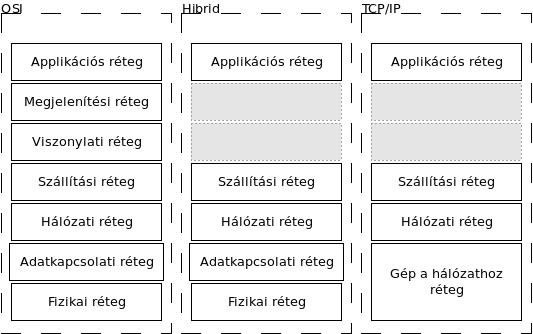
\includegraphics[width=0.6\linewidth]{fig/7-Models}
	\caption{A három modell összehasonlítása}
	\label{fig:7-models}
\end{figure}

A TCP/IP tervezői úgy gondolták, hogy az alkalmazási rétegnek magába kell foglalnia az OSI viszonyrétegének és megjelenítési rétegének részleteit is. Így az általuk létrehozott alkalmazási réteg a megjelenítés, a kódolás és a párbeszédvezérlés kérdéseit kezeli. 

A szállítási réteg a szolgáltatás minőségi kérdéseivel foglalkozik, vagyis a megbízhatósággal, az adatfolyam-vezérléssel és a hibajavítással. Az egyik ide tartozó protokoll, a Transmission Control Protocol (TCP) igen hatékony és rugalmas módon teszi lehetővé a megbízható, gyors, alacsony hibaarányú hálózati kommunikációt. 

A TCP egy összeköttetés alapú (más néven kapcsolatorientált) protokoll. Ez a protokoll párbeszédszerű kommunikációt tart fenn a forrás- és a célállomás között, és szegmensekbe csomagolja az alkalmazási rétegből származó információkat. A kapcsolatorientáltság nem jelenti azt, hogy áramkör létezik a kommunikáló számítógépek között. Azt jelenti, hogy a két állomás között 4. rétegbeli szegmensek haladnak oda-vissza, nyugtázva, hogy bizonyos időtartamra fennáll a logikai összeköttetés.

Az internet réteg rendeltetése, hogy csomagokra bontsa a TCP-szegmenseket, és elküldje őket bármely hálózatról. A csomagok megérkeznek a célhálózatra, attól függetlenül, hogy milyen útvonalon jutottak el oda. Ennek a rétegnek a feladatát az Internetprotokoll (IP) látja el. A legjobb útvonal kiválasztása és a csomagkapcsolás ebben a rétegben történik.

A hálózat-elérési réteg nevének nagyon tág a jelentése, ezért némileg megtévesztő lehet. Másképpen állomás-hálózat közötti rétegnek is nevezzük. Ebbe a rétegbe tartozik minden olyan fizikai és logikai összetevő, amely a fizikai összeköttetés létrehozásához szükséges. Ide tartoznak a hálózati technológiák részletei, beleértve az OSI modell fizikai és adatkapcsolati rétegének minden részletét.

A leggyakrabban használt alkalmazási rétegbeli protokollok közé tartoznak például a következők: 
\begin{itemize}[nosep]
	\item FTP -- File Transfer Protocol (20-21/tcp)
	\item HTTP -- HyperText Transfer Protocol (80/tcp)
	\item HTTPS -- HyperText Transfer Protocol Secure (443/tcp)
	\item SMTP -- Simple Mail Transfer Protocol (25/tcp)
	\item DHCP -- Dynamic Host Configuration Protocol (67-28/udp)
	\item DNS -- Domain Name System (53/udp,tcp)
	\item SFTP -- Secure File Transfer Protocol (22/tcp)
	\item SSH -- Secure SHell (22/tcp)
\end{itemize}

A szállítási réteg gyakoribb protokolljai:
\begin{itemize}[nosep]
	\item TCP -- Transport Control Protocol
	\item UDP -- User Datagram Protocol
\end{itemize}

Az internet réteg a TCP/IP protokollstruktúra fontosabb protokolljai:
\begin{itemize}[nosep]
	\item IP -- Internet Protocol
	\item ICMP -- Internet Control Message Protocol
\end{itemize}
%----------------------------------------------------------------------------
\section{Fizika 1}
{\footnotesize Fizikai fogalmak, mennyiségek. Impulzus, impulzusmomentum. Newton törvényei. Munkatétel. Az I. és II. főtétel. A kinetikus gázmodell.}
%----------------------------------------------------------------------------
\subsection{Fizikai fogalmak, mennyiségek.}
\paragraph{Alapfogalmak}
\begin{description}[nosep]
	\item[Mérőszám] Megmutatja, hogy a mértékegységet hányszor lehet a mérendő mennyiségbe belefoglalni.
	\item[Mértékegység] Egy mérőszám típusát és nagyságrendjét meghatározó jelző.
	\item[Fizikai mennyiség] Adott fizikai jellemzőt leíró mérőszám és annak mértékegysége. Valamely jelenség, folyamat minőségileg megkülönböztethető, és mennyiségileg meghatározható tulajdonsága.
	\begin{enumdescript}[nosep]
		\item[Skalármennyiség] Olyan mennyiség, melynek nincs iránya, tehát teljes mértékben leír a nagysága (pl. hőmérséklet, tömeg, térfogat).
		\item[Vektormennyiség] Olyan mennyiség, melynek nagyságán kívül iránya is van (pl. erő, sebesség, térerősség).
	\end{enumdescript}
\end{description}

\paragraph{Erő}
\emph{Olyan hatás, ami egy tömeggel rendelkező testet gyorsulásra késztet.} Az \emph{eredő erő} a testre ható \emph{összes erő vektoriális összege}. $1N$ erő olyan hatás, amely egy $1kg$$  $ tömegű testet $1\frac{m}{s^2}$ mértékű gyorsulásra késztet. \underline{Vektormennyiség}. Iránya megegyezik a gyorsulás irányával. Néhány alapvető erő: elektromágneses erő, gravitációs erő, nukleáris erő.\\
Jele: $F$ (force) \quad $\vec{F} = m \cdot \vec{a}$\\
Mértékegysége: $N$ (Newton) \quad $ N = \nicefrac{kg\cdot m}{s^2} $

\paragraph{Tömeg}
\emph{A fizikai testek tulajdonsága, amely a tehetetlenségüket méri.} A súlytól eltérően a tömeg mindig ugyanaz marad, akárhová kerül is a hordozója. \underline{Skalármennyiség}.\\
Jele: $m$ (mass)\\
Mértékegysége: $kg$ (kilogramm)

Szigorúan véve három különböző dolgot neveznek tömegnek:
\begin{description}
	\item[Tehetetlen tömeg] a test tehetetlenségének mértéke: a rá ható erő mozgásállapot változtató hatásával szembeni ellenállás. A kis tehetetlen tömegű test sokkal gyorsabban változtatja mozgásállapotát, mint a nagy tehetetlen tömegű.
	\item[Passzív gravitáló tömeg] a test és a gravitációs tér kölcsönhatásának mértéke. Azonos gravitációs térben a kisebb passzív gravitáló tömegű testre kisebb erő hat, mint a nagyobbra.
	\item[Aktív gravitáló tömeg] a test által létrehozott gravitációs tér erősségének a mértéke. Például a Hold gyengébb gravitációs teret hoz létre, mint a Föld, mert a Holdnak kisebb az aktív gravitáló tömege.
\end{description}

\paragraph{Súly}
Az az \underline{erő}, amellyel a test az \textbf{alátámasztást nyomja} vagy a \textbf{felfüggesztést húzza}, tehát \emph{a test környezetére gyakorolt erőinek az eredője}. Azonos tömegű testek különböző erősségű gravitációs terekben különböző súlyúak, mert a testre ható gravitációs erőt a test közvetíti a környezetének.\\
Jele: $G$ \quad $\vec{G} = m \cdot \vec{g}$\\
Mértékegysége: $N$ (Newton)

\paragraph{Távolság}
Két pont közötti távolság az a legrövidebb út, melyen eljutunk egyik pontból a másikba, tehát a helyváltozás mértéke. A legrövidebb út általában egyenes mentén van. \underline{Skalármennyiség}.\\
Jele: $d$ (distance) vagy $l$ (length)\\
Mértékegysége: $m$ (méter)

\paragraph{Pálya}
Azt a vonalat, amin a test mozog, pályának nevezzük.

\paragraph{Út}
A mozgó test által befutott pályaszakasz hossza a megtett út.

\paragraph{Elmozdulás}
A kezdőpontból a végpontba mutató \underline{vektort} elmozdulásnak nevezzük.
Az út hossza nem lehet kisebb az elmozdulás nagyságánál, hiszen két pont között az egyenes szakasznak a legkisebb a hossza.

\paragraph{Idő}
A folyamatokban bekövetkező \emph{események sorrendiségének kifejezésére való skalármennyiség}. Az idő SI-alapegysége az SI-másodperc(?). Az ebből származó nagyobb időegységek, mint perc, óra és nap, nem SI-egységek, mert nem tízes számrendszerűek, és szükség van időnként szökőmásodpercre.\\
Jele: $t$ (time)\\
Mértékegysége: $s$ (szekundum vagy másodperc)

\paragraph{Nyomás}
Az egységnyi felületre ható erőhatást adja meg.\\
Jele: $p$ (pressure) \quad $p = \nicefrac{F}{A}$\\
Mértékegysége: $Pa$ (Pascal) \quad $Pa = \nicefrac{N}{m^2}$

\paragraph{Munka}
Amikor egy \emph{testre kifejtett erő hatására a test elmozdul, mechanikai munkavégzés történik}, ami \underline{arányos} a kifejtett \underline{erő nagyságával} és a \underline{megtett úttal}. A munka az erő és az elmozdulás \underline{skaláris szorzata}. Egy joule munkát végez az egy newton nagyságú erő a vele egyirányú egy méter hosszúságú elmozdulás közben. Ugyancsak egy joule az egy watt teljesítménnyel egy másodpercig végzett munka.\\
Jele: $W$ (work) \quad $W=F\cdot s \cdot \cos\alpha$\\
Mértékegysége: $J$ (Joule)	\quad $J = N \cdot m = kg \cdot \frac{m^2}{s^2}$

\paragraph{Teljesítmény}
A munkavégzés vagy energiaátvitel sebessége, más szóval az \emph{egységnyi idő alatt végzett munka}.\\
Jele: $P$ (power) \quad $P = \nicefrac{W}{t}$\\
Mértékegysége: $W$ (Watt) \quad $W = \nicefrac{J}{s}$

\paragraph{Sebesség}
Egy pontszerű test kitüntetett ponthoz viszonyított mozgásának jellemzésére szolgáló fizikai mennyiség. \textbf{Az út idő szerinti deriváltja}, tehát az \emph{időegység alatt bekövetkezett helyváltozás mértéke}. \underline{Vektormennyiség}.\\
Jele: $v$ (velocity) \quad $v = \nicefrac{s}{t}$\\
Mértékegysége: $\nicefrac{m}{s}$

\paragraph{Gyorsulás}
\textbf{A sebességvektor idő szerinti deriváltja}, tehát az \emph{időegység alatt bekövetkezett sebességváltozás mértéke}. \underline{Vektormennyiség}.\\
Jele: $a$ (acceleration) 
$$\overline{a}=\frac{\Delta v}{\Delta t} = \frac{v-u}{t}\quad \text{ahol v a végsebesség, u a kezdeti sebesség}$$
$$a=\lim\limits_{\Delta t \to 0} \frac{\Delta v}{\Delta t} = \frac{dv}{dt}$$
Mértékegysége: $\nicefrac{m}{s^2}$

\subsection{Impulzus, impulzusmomentum.}
\paragraph{Lendület (impulzus)}
Egy test mozgását leíró vektormennyiség. Nagysága arányos a tömeggel és a sebességgel. Lendületmegmaradás törvénye: zárt rendszer összes lendülete állandó. Nyugalomban lévő testnek nincs lendülete, a lendületet csakis külső erő változtathatja meg.\\
Jele: $p$ (impulzus)	$$\vec{p}=m\cdot \vec{v}$$
Mértékegysége: $kg\cdot \nicefrac{m}{s} = N \cdot s$

\paragraph{Perdület (impulzusmomentum)} Forgómozgásban lévő test lendülete által létrehozott nyomatékot jellemző vektormennyiség. Az erőkar(r) és a lendület(p) \emph{vektoriális szorzata}. Zárt rendszerben a lendületmegmaradás következtében a perdület állandó. Rögzített tengely körüli forgásnál a perdületet a tehetetlenségi nyomaték($\Theta$) és a szögsebesség($\omega$) szorzatából számíthatjuk ki.\\
Jele: $L$	$$\vec{L}=\vec{r}\times\vec{p}\quad L=\Theta \cdot \omega$$
Mértékegysége: $kg\cdot \nicefrac{m^2}{s} = N \cdot m \cdot s$

\subsection{Newton törvényei.}
\begin{description}
	\item[I. Tehetetlenség törvénye] Minden inerciarendszerben vizsgált test nyugalomban marad vagy egyenes vonalú egyenletes mozgást végez mindaddig, míg ezt az állapotot egy másik test vagy erő hatása meg nem változtatja egy kölcsönhatás során.

	\item[II. Dinamika alaptörvénye] Egy pontszerű test gyorsulása azonos irányú a rá ható erővel, nagysága egyenesen arányos az erő nagyságával, és fordítottan arányos a test tömegével. $\vec{F}=m \cdot \vec{a}$

	\item[III. Hatás-ellenhatás törvénye] Két test kölcsönhatása során mindkét testre azonos nagyságú, azonos hatásvonalú és egymással ellentétes irányú erő hat.

	\item[IV. Szuperpozíció elve] Ha egy testre egy időpillanatban több erő hat, akkor ezek együttes hatása megegyezik a vektori eredőjük (vektoriális összegük) hatásának vonalával.
\end{description}

\subsection{Munkatétel.}
\begin{theorem}
	Egy test mozgási energiájának változásának mértéke megegyezik a testre ható összes erő munka előjeles összegével.
	$$\Delta E_m = \sum_{i=1}^{n}W_i$$
\end{theorem}

\subsection{A termodinamika I. és II. főtétel.}
\begin{theorem}[I. főtétel]
	Egy zárt rendszer belső energiájának változása egyenlő a rendszerrel közölt hő és a rendszeren végzett munka összegével.
	$$ \Delta U = Q+W $$
\end{theorem}
A testek belső energiájának megváltozása egyenlő a testtel közölt hőmennyiség és a testen végzett munka előjeles összegével. Ez az energiamegmaradás törvénye, mert azt mondja ki, hogy külső beavatkozás nélkül nincs energiaváltozás.

\begin{theorem}[II. főtétel]
	Termikus kölcsönhatással járó természetes folyamatoknál csak a nagyobb hőmérsékletű test képes a hőátadásra. Tehát egy elszigetelt rendszer állapota időben termikus egyensúly felé halad.
\end{theorem}

\subsection{A kinetikus gázmodell.}
A gázok tömeggel rendelkező részecskékből állnak, melyek energiaveszteség nélkül ütköznek egymással és a környezetükben lévő testekkel. Mozgási energiájuk csak a rendszer hőmérsékletétől függ. Állandóan mozgásban vannak, és az ütközések között egyenes vonalú egyenletes mozgást végeznek. Össztérfogatuk mindig jóval kisebb, mint a gázt tartalmazó tároló térfogata.
Alapegyenlet: $$p \cdot V = \frac{2}{3}N \cdot \frac{1}{2}mv^2$$ ahol p az ütközésekkel keltett nyomás, V a térfogat, N a molekulaszám, az $\nicefrac{1}{2}mv^2$ pedig egy molekula átlagos mozgási energiája.

A kinetikus gázmodell segítségével értelmezhetők a gázok olyan makroszkopikus tulajdonságai, mint a nyomás, a hőmérséklet, vagy a térfogat. Newton úgy gondolta, hogy a gáz nyomását a molekulái között fellépő állandó taszítás okozza, a kinetikus gázelmélet szerint viszont a nyomás a különböző sebességgel mozgó gázmolekulák ütközéseiből származik. A kinetikus gázmodell a természetben nem létező ideális gázt feltételez.
A kinetikus gázmodell szerint:
\begin{enumerate}
	\item a gáz részecskékből áll, amelyeknek tömege és súlya van, viszont össztérfogatuk elhanyagolható a gázt tartalmazó edény térfogatához képest
	\item a részecskék állandó mozgásban vannak
	\item a részecskék tökéletes gömb alakúak és rugalmas természetűek
	\item a részecskék mozgási energiája csak a rendszer hőmérsékletétől függ
	\item a részecskék egymással és az edény falával energiaveszteség nélkül ütköznek
	\item a részecskék közötti erőhatások elhanyagolhatóak, ezért két ütközés között egyenes vonalú egyenletes mozgást végeznek
\end{enumerate}
A kinetikus gázelmélet alapegyenlete:
$$ pV = \frac{2}{3}N \frac{m_0v^2}{2}$$
$p$ – nyomás
$V$ – térfogat
$N$ – molekulák száma
$m_0$ – egy molekula tömege
$\frac{m_0v^2}{2}$– egy molekula átlagos mozgási energiája
%----------------------------------------------------------------------------
\section{Fizika 2}
{\footnotesize Elektromos alapfogalmak és alapjelenségek. Ohm-törvény. A mágneses tér tulajdonságai. Elektromágneses hullámok. A Bohr-féle atommodell. A radioaktív sugárzás alapvető tulajdonságai.}
%----------------------------------------------------------------------------
\subsection{Elektromos alapfogalmak és alapjelenségek.}
\subsubsection{Testek elektromos állapota}
Minden atom magja pozitív töltésű protonokból és töltés nélküli neutronokból áll. A mag körüli elektronhéjon keringenek a protonokkal megegyező számú, negatív töltésű elektronok.\\
Alapesetben az atom kifelé elektromos hatást nem mutat. Ha elektronokat ad le vagy vesz fel, akkor viszont pozitív, illetve negatív töltésű ionná válik. Ennek megfelelően megkülönböztetünk pozitív, negatív és semleges elektromos állapotot.\\
Elektromos szempontból az anyagokat vezetőkre és szigetelőkre oszthatjuk. Az elektromos vezetők mozgásképes töltéshordozókat (elektronokat, ionokat) tartalmaznak. Megkülönböztetünk elsőrendű vezetőket (fémek és a szén), másodrendű vezetőket (elektrolitok és ritkított gázok), félvezetőket, (pl. germánium, szelén, szilícium) amelyek kristályos szerkezetű anyagok és részben vezetők, részben szigetelők. Speciálisak a szupravezetők, amelyek hőmérsékletét csökkentve, a kritikus hőmérséklet elérésekor hirtelen teljesen elvesztik ellenállásukat. Az elektromos szigetelők (pl. üveg, olaj, műanyag) nem tartalmaznak mozgásképes töltéshordozókat.

\subsubsection{Elektromos töltés}
Az anyag alapvető tulajdonsága, bizonyos elemi részecskék jellemzője. Megkülönböztetünk pozitív és negatív töltést. Azonos nemű töltések taszítják, különböző neműek vonzzák egymást.\\
Jele: Q\\
Mértékegysége: Coulomb (C)\\
1 Coulomb = 1As (amperszekundum)\\
Az elektromosan töltött anyag elektromágneses teret hoz létre. Az elektromos töltés kvantált, azaz minden test töltése egy legkisebb töltés többszöröse. Ez a legkisebb töltés az elemi töltés, ami a proton töltése: 1,6 · 10 -19 Coulomb. Az elektron töltése ennek a -1 -szerese. (A kvarkok felfedezése óta úgy gondolják, hogy azok töltése még kisebb lehet, az elemi töltés 1/2, vagy 1/3 része.) Az elektromos töltésre is igaz a megmaradási elv, azaz zárt rendszer töltése állandó. Az elektromos töltések egymásra gyakorolt erőhatásán keresztül a töltés mérhető. A pontszerű töltések között ható (F) erő egyenesen arányos a töltésekkel (Q 1 , Q 2 ) és fordítottan arányos a töltések közötti
távolság (r) négyzetével. Ez Coulomb törvénye:
$$F=k\cdot\frac{Q_1 \cdot Q_2}{r^2}$$
ahol $k$ az arányossági tényező, melynek értéke: $9\cdot10^9 \frac{Nm^2}{C^2}$

\subsubsection{Elektromos Térerősség}
Két pontszerű töltés egymásra gyakorolt hatását úgy is értelmezhetjük, hogy az egyik töltés maga körül elektromos teret hoz létre és ebben a térben a másik töltésre erő hat. Ez az $F$ erő arányos a térben lévő $Q$ töltés nagyságával:
$$F=Q\cdot E$$
Az $E$ arányossági tényező jellemzi az elektromos teret, neve elektromos térerősség. Vektormennyiség, ha a $Q$ töltés pozitív, akkor a töltésre ható erő iránya megegyezik $E$ irányával.
Mértékegysége:$\nicefrac{N}{C}$ és $\nicefrac{V}{m}$

\subsubsection{Fluxus}
Az elektromos mezőt erővonalakkal (Faraday vonalak) szemléltetjük. Az erővonalak bármely pontjába húzott érintő megadja az adott pontban mérhető térerősség irányát, a vonalak sűrűsége pedig a térerősség nagyságával arányos. A fluxus az erővonalak száma. Jele a $\Psi$ (pszi), mértékegysége:$\frac{N}{C}m^2$.
$$ \varPsi = E \cdot A = 4k \cdot \pi \cdot Q $$
$E$ : $Q$ elektromos töltéstől $r$ távolságban a térerősség ($k\frac{Q}{r^2}$)\\
$A$ : egy $r$ sugarú gömb felszíne ($4\pi r^2$)
\begin{theorem}[Gauss-tétel]
	Zárt felületen az elektromos tér fluxusa egyenlő a felületen belül elhelyezkedő töltés $4k\pi$–szeresével. Ha $Q$ pozitív, akkor az erővonalak a felületről kifelé, ha negatív, akkor befelé irányulnak. Tehát minden $Q$ pozitív töltésből $4k\pi Q$ erővonal indul és minden $Q$ negatív töltésben $4k\pi Q$ erővonal végződik.
\end{theorem}

\subsubsection{Elektromos potenciál és feszültség}
Az elektromos mező erőt fejt ki a benne mozgó töltött testre, ezért munkát végez azon. A végzett munka kiszámolható, ha ismert a két (A és B) pont közti feszültség. A feszültség jele: $U$, mértékegysége volt (V). Mindig két pont között értendő. $U=U(A,B)$.
Ha a test töltése Q coulomb, akkor az elektromos mező éppen
$$W=Q \cdot U $$
munkát végez a töltött testen, miközben az a mező A pontjából a mező B pontjába mozdul el. 

Az elektromos mező, vagy elektromos hálózat egy adott pontjának potenciálja az adott pontnak egy választott 0-ponthoz  viszonyított feszültsége. A 0-pont megválasztása tetszőleges. Képlettel: 
$$U(A)=U(A,0)$$
Az azonos potenciálú pontok között mozgó töltött testen az elektromos tér nem végez munkát, azokat nem gyorsítja vagy lassítja. Az azonos potenciálú pontok ekvipotenciális vonalakat, felületeket alkotnak. Ezek jól ábrázolják az elektromos teret. Praktikusan a Föld-et tekintik 0-potenciálú testnek, így a Földdel vezetékkel összekötött fémek potenciálja nulla lesz. A potenciál ilyen módon való lenullázása a földelés. 

Pontszerű töltés által $r$ távolságra keltett feszültség:
$$U(r)=k\cdot\frac{Q}{r} \quad \text{(előjelesen)}$$
%Ebből a potenciál:
%$$U = k\cdot \frac{Q}{r}$$
%Az elektromos teret egy kiválasztott pontjához képest fennálló munkavégző képessége szempontjából a potenciál jellemzi. A villamos töltések a villamos tér egyes pontjaiban potenciális energiával rendelkeznek.
%Az elektromos tér valamely pontjának potenciálja az a munkamennyiség, amellyel a tér az egységnyi pozitív töltést abból a pontból a nullapotenciálúnak választott pontba képes mozgatni.
%Az elektromos tér két pontja közötti feszültség az a munkamennyiség, amellyel a tér az egységnyi pozitív töltést a nagyobb potenciálú pontból a kisebb potenciálú pontba képes mozgatni. A feszültség tehát a két
%pont potenciáljának különbsége. 
%Így az A és B pont közötti feszültség az A-ból a B-be történő mozgatáshoz szükséges munka és a mozgatott töltés hányadosa:
%$$U_{AB} = U_A - U_B = \frac{W_{AB}}{Q}$$
%Mértékegysége a Volt. Az elektromos mező két pontja között 1 Volt a feszültség, ha 1 Coulomb töltés átvitelekor az erők 1 Joule munkát végeznek.

\subsubsection{Elektromos áram és áramerősség}
Az elektromos áram a szabadon mozgó töltéshordozók rendezett áramlása. Az elektromos áram létrejöttének feltétele a potenciálkülönbség. Ha az áramlás folyamatosan egyirányú, akkor egyenáramról, ha az áramlás iránya szabályos időközönként megfordul, akkor váltakozóáramról beszélünk.\\
Egyenáram esetén az áramerősség a vezető keresztmetszetén t idő alatt átáramló töltések mennyisége:
$$ I = \frac{Q}{t}$$

Mértékegysége az Amper.
1 Ampernyi áramerősség a vezetőréteg keresztmetszetén 1 sec alatt átáramló 1 Coulomb töltést jelent.

\subsubsection{Kapacitás}
Egy áramköri elem azon képessége, hogy mennyi elektromos töltést képes tárolni. Két vezetőből álló kondenzátor esetén a kapacitás egyenlő az egyik vezetőn felhalmozott töltés és a vezetők közötti feszültség hányadosával:
$$ C = \frac{Q}{U} $$
Mértékegysége a Farad.

\subsubsection{Ohm-törvény}
Egy áramkörben az áramerősség állandó nagyságú ellenállás esetén egyenesen arányos a feszültséggel:
$$U = I \cdot R \quad R = \frac{U}{I}$$
$R$ az ellenállás, ami a vezető anyagi minőségétől, méreteitől és hőmérsékletétől függő állandó.\\
Mértékegysége az Ohm ($\Omega$).\\
1 Ohm ellenállású a vezető, ha abban 1 Volt feszültség 1 Amper erősségű áramot hoz létre.\\
Az ellenállás a vezető hosszával egyenesen, a keresztmetszetével fordítottan arányos:
$$ R = \rho \cdot \frac{l}{A} $$
$\rho$ (ró) a vezető fajlagos ellenállása, ami az anyagi minőségétől és hőmérsékletétől függő állandó.

\subsubsection{Elektromos áram munkája és teljesítménye}
A feszültség: $U = \frac{W}{Q} \rightarrow W = U \cdot Q$\\
Az áramerősség: $I = \frac{Q}{t} \rightarrow Q = I \cdot t$\\
\textbf{Elektromos munkavégzés:} $W = U \cdot I \cdot t$\\
Másképpen: $U = IR,\;I=\frac{U}{R} \rightarrow W = I^2R\cdot t = \frac{U^2}{R} \cdot t$\\
\textbf{Elektromos teljesítmény:}$P=\frac{W}{t}=\frac{UI\cdot t}{t} \rightarrow P=U\cdot I = I^2\cdot R = \frac{U^2}{R}$\\
Az elektromos teljesítmény általános mértékegysége a kilowatt (kW), a munkáé pedig a kilowattóra (kWh).

\subsection{A mágneses tér tulajdonságai. }
Két mágnesrúd egymásra vonzó vagy taszító hatást fejt ki. Az azonos mágneses pólusok taszítják, az ellentétesek vonzzák egymást. Ebből következik, hogy minden mágnes maga körül -- az elektromos erőtérhez hasonlóan -- mágneses erőteret létesít. Az erőteret a térerősséggel, a mágneses indukcióval jellemezhetjük és erővonalakkal szemléltethetjük (\ref{fig:9-eathmagneticfield}~ábra).
\begin{figure}[h]
	\centering
	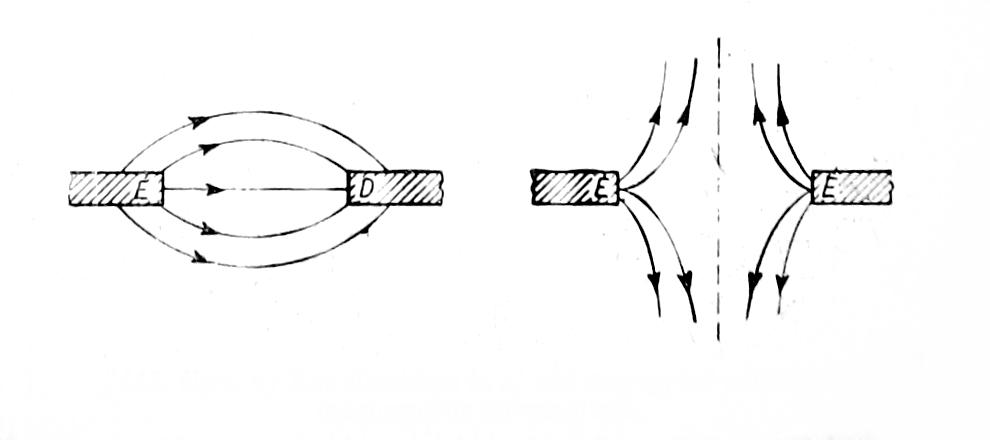
\includegraphics[width=0.7\linewidth]{fig/9-Magnetic_field}
	\caption{}
	\label{fig:9-magneticfield}
\end{figure}

Az erővonalak olyan görbék, amelyek a mágnesben záródnak és irányuk a térben az északi pólustól a déli pólus felé mutat. Ha az erővonalak párhuzamosak és mindenütt egyenlő sűrűségűek, akkor a mágneses tér homogén. A mágneses tér és az elektromos tér legfőbb különbsége, hogy míg az elektromos teret akár a pozitív, akár a negatív töltés egymagában is létrehozza, addig a mágneses teret az északi és déli pólus mindig együttesen létesíti.

Abból, hogy a vízszintes síkban szabadon forgó mágnes mindig észak-déli irányba áll be az következik, hogy a Föld is egy mágnes. A Föld északi sarkán déli, déli sarkán északi mágnesség van. Ezért az erővonalak iránya délről észak felé mutat (lásd:\ref{fig:9-eathmagneticfield}~ábra).
\begin{figure}[h]
	\centering
	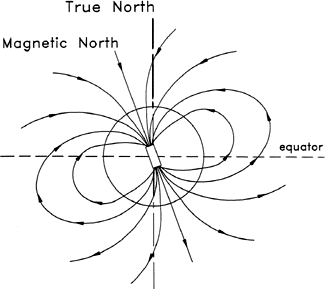
\includegraphics[width=0.3\linewidth]{fig/9-Eath_magnetic_field}
	\caption{}
	\label{fig:9-eathmagneticfield}
\end{figure}

Ha egy vezetőben áram folyik, akkor az mágneses erőteret hoz létre maga körül. A mágneses erővonalak a vezetőre merőleges síkban kialakuló koncentrikus körök, amelyek sűrűsége a vezetőtől távolodva csökken. Az erővonalak irányát jobb kezünk behajlított ujjainak iránya adja, ha hüvelykujjunk az áram irányába mutat. Ha tehát az áram iránya megváltozik, az erővonalak iránya is ellentétessé válik (Jobbkéz-szabály).
\begin{theorem}[Biot--Savart-törvény]
A mágneses térerősség jele $H$. Ha a vezetőben $I$ az áramerősség és $\alpha$ az irányszög, akkor a vezető $\Delta L$ hosszúságú szakasza által, tőle $r$ távolságban létrehozott térerősség nagysága:
$$H=\frac{\mu_0}{4\pi}\cdot\frac{I\cdot \Delta L}{r^2}\cdot \sin \alpha$$
$\mu_0$: permeabilitás
\end{theorem}
A térerősség mértékegysége az Amper/méter.

Egy többmenetes hengeres tekercs mágneses erővonalai az egyes menetek mágneses terének eredőjeként alakulnak ki. Mivel a tekercs belsejében a mágneses tér majdnem homogén, a tekercs egy olyan rúdmágnesnek tekinthető, amelynek hossztengelye egybeesik a tekercs tengelyével (lásd:\ref{fig:9-coil}~ábra).
\begin{figure}[h]
	\centering
	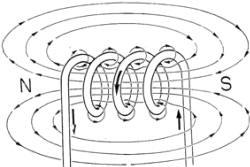
\includegraphics[width=0.3\linewidth]{fig/9-Coil}
	\caption{}
	\label{fig:9-coil}
\end{figure}
Ha egy $N$ menetszámú tekercsben $I$ az áramerősség és a tekercs hossza $L$, akkor a tekercsben a mágneses térerősség:
$$H = \frac{I\cdot N}{L}$$
Ha egy két végén hintaszerűen felfüggesztett vezetőt egy mágnes erőterébe helyezünk és a vezetőn az áramot bekapcsoljuk, akkor a vezető az áram irányára merőleges irányba mozdul ki. Az elmozdulást létesítő $F$ erő nagysága:
$$ F = B \cdot I \cdot L $$
$I$ az áramerősség, $L$ a vezetőnek a mágneses térbe eső hossza, $B$ pedig a mágneses térben lévő anyagtól függő állandó, a mágneses indukció melynek mértékegysége a Tesla.

A mágneses indukciót indukcióvonalakkal jellemezhetjük. Egy adott felületen áthaladó indukcióvonalak száma a mágneses fluxus, ami az indukció és a felület szorzata: $f = B\cdot A$\\
A mágneses fluxus mértékegysége a Weber.

\subsection{Elektromágneses hullámok. }
Az elektromos töltéssel rendelkező testeknek a töltésük miatt fellépő kölcsönhatását az elektromos és mágneses tér segítségével írhatjuk le. A kölcsönhatás úgy működik, hogy egyrészt minden töltés maga körül elektromágneses teret hoz létre, másrészt az elektromágneses tér a töltésekre erőt fejt ki. Így azt mondhatjuk, hogy két töltött test kölcsönhatása az elektromágneses tér közvetítésével valósul meg. Az elektromágneses tér létrehozásához munkát kell végezni, amely munka révén a létrehozott elektromágneses térben energia halmozódik fel. Tudjuk, hogy az elektromágneses tér időbeli változása a térben meghatározott sebességgel (fénysebességgel, amely vákuumban 300 000 km/s) tovaterjed: elektromágneses hullám jön létre, ami energiát visz magával, az elektromágneses tér energiájának sajátos transzportja jön létre. Az elektromágneses hullám energiaszállító képességére utal az elektromágneses sugárzás elnevezés. Egy hozzánk képest nyugvó elektromos töltés elektromos teret, egyenletesen mozgó töltés elektromos és mágneses teret hoz létre maga körül. Kimutatható, hogy a fenti két esetben a tér és a benne felhalmozott energia a töltéstől nem szakítható el, mintegy hozzá van láncolva. Ha azonban a töltés gyorsul, akkor a körülötte kialakuló, időben változó elektromágneses tér elektromágneses hullámot kelt, amely a töltésről leszakadva a térben tovaterjed, és energiát visz magával: a gyorsuló töltés elektromágneses sugárzást bocsát ki magából. Elektromos töltéssel rendelkező testek azonban nemcsak sugározni képesek, hanem a rájuk eső elektromágneses sugárzást el is nyelhetik. Ha ugyanis az anyag egy töltött részecskéjét elektromágneses sugárzás éri, akkor a sugárzás elektromágneses tere a tér által a töltésre ható erő révén a részecskét felgyorsítja, miáltal a test a ráeső sugárzás egy részét elnyeli. A fenti két folyamat teszi lehetővé, hogy két test kölcsönhatásba léphet egymással úgy is, hogy az egyik a másiknak elektromágneses sugárzás formájában energiát ad át. Ennek a jelenségnek számos konkrét példáját ismerjük. Az elektromágneses sugárzás útján történő energiaátadás közismert példája az elektromágneses hullámokkal megvalósított távközlés (rádió, TV): egy rádióadóban pl. a továbbítandó elektromos jellel (váltakozó áram) rezgőmozgásba (gyorsuló mozgás) hozzák az adóantenna elektronjait, amelyek ennek megfelelő elektromágneses sugárzást bocsátanak ki. Ennek a sugárzásnak egy része eléri a vevőkészülék antennáját, és a benne lévő elektronokat a sugárzás elektromos tere rezgésbe hozza. Az elektronoknak ez a rezgőmozgása (váltakozó áram) azután a vevőkészülékben létrehozza a leadott jelnek megfelelő elektromos jelet. A sugárzásos energiaátadás másik, közismert példája a hőmérsékleti sugárzás kibocsátása és elnyelése. Tapasztalati tény, hogy az anyagok a hőmérsékletüktől függően különböző hullámhosszú elektromágneses sugárzást bocsátanak ki magukból, s a rájuk eső sugárzás egy részét elnyelik.

A foton az elektromágneses hullámok elemi részecskéje. A fotonok nyugalmi tömege nulla, sebességük a fénysebesség. Az elektromágneses hullám keletkezése atomi szinten úgy történik, hogy a gerjesztés hatására az atommag körül keringő elektron egy nagyobb energiájú pályára ugrik, majd onnan eredeti pályájára visszazuhanva egy fotont bocsát ki. A keletkező foton hullámhossza az energiaszintek különbségétől függ.

A különböző körülmények között létrejött elektromágneses sugárzások lényegében a kibocsátott hullám hullámhosszában és ezzel együtt frekvenciájában térnek el egymástól, és ez eredményezi azt, hogy az anyaggal való kölcsönhatásaik, az anyagra gyakorolt hatásaik is eltérőek.Az elektromágneses sugárzás hullámhossz szerinti felosztása, az ún. elektromágneses spektrum (lásd:\ref{fig:9-electromagneticspectrum}~ábra)
\begin{figure}[h]
	\centering
	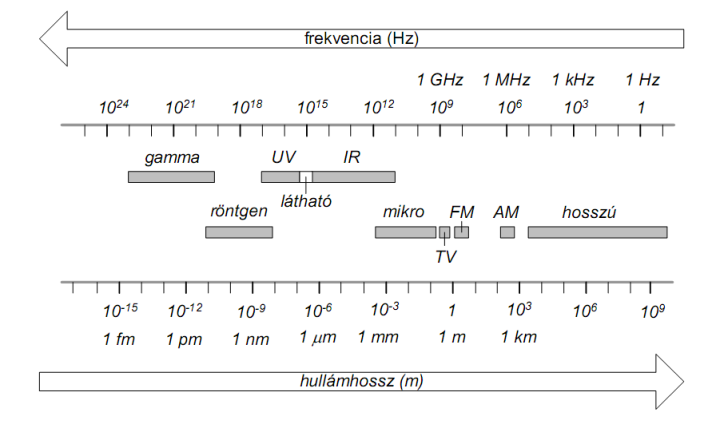
\includegraphics[width=0.7\linewidth]{fig/9-Electromagnetic_spectrum}
	\caption{}
	\label{fig:9-electromagneticspectrum}
\end{figure}

A fény szűkebb értelemben az elektromágneses spektrumnak az a része, amelyet az emberi szem érzékelni képes (kb. 350-től 750 nanométerig). Tágabb értelemben ide sorolják a tartományhoz közvetlenül csatlakozó hosszabb hullámhosszú infravörös- és a rövidebb hullámhosszú ultraibolya sugárzást is. Az emberi szem érdekes sajátsága, hogy a különböző hullámhosszú fényt különböző színűnek észleli. A klasszikus felfogás szerint a fényhullámként terjed, tehát érvényesek rá mindazok az általános törvények, amelyek a hullámokra érvényesek. A fénynek azonban vannak, elektromágneses jellegével és a hullámhosszával összefüggő, speciális tulajdonságai is.

A fény egy anyagban terjedve, és egy határfelülethez érve részben behatol az új anyagba, részben pedig visszaverődik a határfelületről. Vannak anyagok, amelyekbe a fény gyakorlatilag nem tud behatolni, mert a határfelületeikről a fénysugárzás nagyobb része visszaverődik, vagy igen rövid távolságon belül elnyelődik. Az anyagok egy része a fényt többé-kevésbé átereszti, ezeket az anyagokat legtöbbször átlátszó anyagoknak nevezzük. A fény és anyag kölcsönhatása általában függ a fény hullámhosszától, így egy anyag bizonyos hullámhosszakra lehet áteresztő, más hullámhosszakat viszont elnyel.

Az elektromágneses hullámok létezését elméletben Maxwell (1864), kísérletileg Hertz mutatta ki (1888).

\subsection{A Bohr-féle atommodell.}
Az 1900-as évek elején Ernest Rutherford megalkotta róla elnevezett atommodelljét, amely szerint az atom középpontjában van a pozitív töltésű atommag, ami körül keringenek az elektronok. Az atom kifelé semleges, tehát az elektronok száma egyenlő az atommag pozitív töltésének a számával. A modell legnagyobb hibája az volt, hogy mivel a keringő elektronok váltakozó elektromágneses teret hoznak létre maguk körül, ezzel együtt energiát kell kisugározniuk, viszont az energia kisugárzás csökkenti az elektron mozgási energiáját, így az elektron egy idő után az atommagba kellene, hogy essen.

1913-ban Niels Bohr dán fizikus a Rutherford-féle atommodell módosításával megalkotta saját atommodelljét, amely szerint:
\begin{enumerate}[nosep]
	\item Az atom normális (gerjesztés nélküli) állapotában az elektron csak meghatározott pályán keringhet és 	ebben az esetben nem sugároz energiát. Emellett azt is feltételezte, hogy az elektronpályák sugarai úgy aránylanak egymáshoz, mint a természetes egész számok négyzetei:
	\begin{figure}[h]
		\centering
		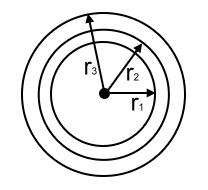
\includegraphics[width=0.25\linewidth]{fig/9-Atom_eletrontracks}
		\caption{$r_1 : r_2 : r_3 = 1 : 4 : 9$}
		\label{fig:9-atomeletrontracks}
	\end{figure}
	
	\item A megengedett pályákon keringő elektronoknak meghatározott energiájuk van, amelyet mozgási energiájuk és az elektromos erőtér potenciális energiája határoz meg. Egy elektron összenergiája a nagyobb sugarú pályán nagyobb.
	\item Ha az atommal energiát közlünk, akkor az elektron átugrik egy másik, nagyobb sugarú pályára. Ez az ún. gerjesztés. A gerjesztéskor felvett energia megegyezik a két pályához tartozó energiaértékek különbségével. A gerjesztett atom azonban instabil, így az elektron a nagyobb energiájú pályáról a maghoz közelebbi kisebb energiájú belső pályára ugrik és az energiakülönbséget elektromágneses hullám formájában kisugározza.
\end{enumerate}

\subsection{A radioaktív sugárzás alapvető tulajdonságai.}
Becquerel francia fizikus 1896-ban kutatásai során megállapította, hogy az uránszurokérc olyan sugarakat bocsát ki magából, amelyeknek nagy az áthatolóképességük, a levegőt ionizálják. Két évvel később a Curie házaspárnak sikerült az uránércből az uránnál kb. milliószor erősebben sugárzó anyagot a rádiumot kiválasztani. Később még ennél is erősebben sugárzó anyagot találtak, ez a polónium. A további kutatások során megállapították, hogy ilyen radioaktív sugarakat még sok más elem is kibocsát és ezekre az anyagokra jellemző, hogy külső behatás nélkül, állandóan sugároznak.

A radioaktív sugárzás a radioaktív bomlás során keletkezik. A bomlás izotópokban megy végbe. Majdnem valamennyi a természetben előforduló elem izotópok keverékéből áll. Egy elem izotópjai, az elemmel azonos rendszámú, de eltérő tömegszámú és atomsúlyú elemek. Egy adott elem mindegyik izotópja ugyanannyi protont és elektront, de eltérő számú neutront tartalmaz. Egy elem izotópjai kémiailag teljesen azonosak, de fizikai tulajdonságaik eltérnek. Azokat, amelyeknél nem figyeltek meg radioaktív bomlást, stabil izotópoknak nevezik, míg, amelyeknél megfigyeltek azok instabil izotópok. Egy elem csak meghatározott proton/neutron arány esetén stabil. Nagyon sok elemnek vannak természetes radioaktív izotópjai. Vannak olyan elemek, amelyeknek csak radioaktív izotópja létezik (pl. polónium, radon, rádium), viszont mesterségesen minden elemnek előállítható radioaktív izotópja.

A radioaktív bomlás során a radioaktív izotópok instabil atomjai hosszabb-rövidebb idő elteltével alacsonyabb energiaszintű állapotba mennek át, és eközben emberi érzékszervekkel nem észlelhető, de műszerekkel jól kimutatható radioaktív sugárzást bocsátanak ki.

A bomlás mértéke lemérhető. Az 1 másodperc alatt bekövetkező bomlások száma az aktivitás. Mértékegysége a Becquerel. 1 Bq = 1 bomlás/másodperc.

A bomlást a felezési idővel is jellemezhetjük, ez az az idő, amely alatt egy bizonyos mennyiségű anyag atomjainak a száma radioaktív bomlással a felére csökken. Másodpercektől éves nagyságrendekig változhat, akár sok millió vagy milliárd év is lehet.

A bomlás során keletkező sugárzásnak 3 fajtáját különböztetjük meg:
\begin{description}
	\item[Alfa-sugárzás] Pozitív töltésű héliumionokból áll. Töltésük az elemi töltés kétszerese, tömegük kb. a hidrogénatom tömegének négyszerese, sebességük függ a kibocsátó anyagtól. Az alfa-sugaraknak nagy az áthatolóképességük és erősen ionizálnak, viszont a levegőmolekulákkal való ütközés során hamar lefékeződnek, így hatótávolságuk kevesebb, mint egy centiméter.
	\item[Béta-sugárzás] elektronok vagy pozitronok (béta-részecskék) alkotják. Sebességük széles skálán változik, de jóval nagyobb, mint az alfa-sugárzás esetében és bár tömegük jóval kisebb, mint az alfa-részecskék tömege, a nagy sebesség miatt hatótávolságuk levegőben néhányszor tíz centiméter.
	\item[Gamma-sugárzás] agy energiájú elektromágneses sugarak, frekvenciájuk elérheti a 10\textsuperscript{21} Hz értéket. Hatótávolságuk végtelen, a nagy tömegszámú és sűrűségű elemek (pl. ólom) viszont hatékonyan gyengítik.
\end{description}
A bomlásokat az általuk létrehozott sugárzás alapján különböztetjük meg. Eszerint van alfa-, béta- és gamma-bomlás.
%----------------------------------------------------------------------------
\section{Elektronika 1, 2}
{\footnotesize Passzív áramköri elemek tulajdonságai, RC és RLC hálózatok. Diszkrét félvezető eszközök, aktív áramköri elemek, alapkapcsolások. Integrált műveleti erősítők. Tápegységek. Mérőműszerek.}
%----------------------------------------------------------------------------
\subsection{Passzív áramköri elemek tulajdonságai, RC és RLC hálózatok.}
\paragraph{Ellenállás}
Jele: $R$\\
Kiszámítása: $R = \nicefrac{U}{I}$\\
Az ellenállás kapcsolata a teljesítménnyel: $P=\nicefrac{U^2}{R}\quad P=U \cdot I$\\
\begin{itemize}[nosep]
	\item Állandó értékű ellenállások
	\begin{itemize}[nosep]
		\item Felépítés: szigetelő hordozó, vezető réteg, fém kivezetések
		\item Főbb típusok: huzalellenállás, rétegellenállás, tömbellenállás
		\item Beszerelés: furatba, felületre (SMD)
		\item Értékét Ohm-ban [$\Omega$] adják meg  $\rightarrow R = \rho \cdot \nicefrac{l}{A}$ alapján
		\item Névleges érték, tűrés $\rightarrow$ nem tudják pontosan gyártani őket, ezért van egy tűréshatár \%-ban
		\item Terhelhetőség: Watt-ban, maximális teljesítménye; az ellenállás melegszik $\rightarrow$ hődisszipáció
		\item Ellenálláskódok $\rightarrow$ ellenálláson színkódok és számkódok
	\end{itemize}
	\item Változtatható ellenállások (potenciométerek)
	\begin{itemize}[nosep]
		\item Típusok: huzalpotenciométer, rétegpotenciométer
		\item Szabályozási jellemző: lineáris, nem lineáris (logaritmikus, fordított logaritmikus, S alakú)
		\item Terhelhetőség: a teljes névleges ellenállásra vonatkozik, az ebből számított áramot a csúszka egyik állásában sem haladhatja meg a potenciométer árama $$I_{\max} = \sqrt{\frac{P}{R_\text{névleges}}}$$
	\end{itemize}
	\item Speciális ellenállások (PTK, NTK, VDR)
\end{itemize}

\paragraph{Kondenzátor}
Jele: $C$\\
Kiszámítása: $Q = C \cdot U$\\
Mértékegysége: $\nicefrac{As}{V} =$ Farad
\begin{itemize}[nosep]
	\item Állandó kapacitású kondenzátorok
	\begin{itemize}[nosep]
		\item Felépítés: fém fegyverzetek, fém kivezetések, dielektrikum
		\item Főbb típusok: sík, hengeres, tekercselt, többrétegű
	\end{itemize}
	\item Változtatható kondenzátorok
	\begin{itemize}[nosep]
		\item Felépítés: mozgatható fegyverzetek, légrés (a fegyverzetek alakja határozza meg a szabályozási jelleget)
	\end{itemize}
\end{itemize}

\paragraph{Tekercs}
Jele: L\\
Kiszámítása: $B = \nicefrac{\Phi}{A}$\\
\begin{description}[nosep]
	\item[Indukció] a tekercsben feszültség jön létre, ha a tekercsen átmenő fluxus megváltozik.
	\item[Önindukció] feszültség indukálódik a tekercsben akkor is, ha a fluxus változását áramának megváltoztatásával saját maga idézte elő.
\end{description}
\textbf{A feszültség azért jön létre, mert megváltozik az áram folyásának iránya, mert ilyenkor a fluxus is megváltozik.}

\paragraph{Transzformátor}
Magyar találmány: Bláthy-Zipernowsky-Déry. Zárt vasmag, két oldal: primer és szekunder tekercs. $$ \frac{U_1}{U_2} = \frac{N_1}{N_2}$$
ahol $N$ a tekercs menetszáma.\\
Felhasználás: igény szerinti feszültség előállítás a 230V-os hálózati feszültségből és a villamos energia gazdaságos szállítása.

\begin{theorem}[Kirchhoff I. törvénye]
	Egy csomópontba befolyó áramok összege megegyezik az onnan elfolyó áramok összegével. (csomóponti törvény) $$ \Sigma I = I_1 + I_2 + I_3 + \dots$$
\end{theorem}

\begin{theorem}[Kirchhoff II. törvénye]
	Bármely zárt hurokban az áramköri elemeken lévő feszültségek előjel helyesen vett összege nulla. (hurok törvény) $$ \Sigma U = 0 $$
\end{theorem}

\paragraph{Soros kapcsolás}
Soros kapcsolásban ugyanaz az áram folyik át minden ellenálláson, a feszültségek
összeadódnak. A sorosan kapcsolt ellenállások eredőjét az ellenállások összegzésével kapjuk, így az eredő nagyobb lesz bármely elem értékénél.
$$R_e = R_1 + R_2 + R_3\quad 
L_e = L_1 + L_2 + L_3\quad 
\frac{1}{C_e} = \frac{1}{C_1} + \frac{1}{C_2} + \frac{1}{C_3}$$

\paragraph{Párhuzamos kapcsolás}
Párhuzamos kapcsolásban azonos feszültség lép fel minden ellenálláson, az áramerősségek pedig összeadódnak. A párhuzamosan kapcsolt ellenállások eredőjét az ellenállások reciprokának összegével képezzük, ami még nem az eredőt,hanem annak a reciprokát adja ezért ennek is venni kell még a reciprokát.
$$\frac{1}{R_e} = \frac{1}{R_1} + \frac{1}{R_2} + \frac{1}{R_3}\quad \frac{1}{L_e} = \frac{1}{L_1} + \frac{1}{L_2} + \frac{1}{L_3}\quad 
C_e = C_1 + C_2 + C_3$$
%Párhuzamosan kapcsolt ellenállások, induktivitások, illetve sorosan kapcsolt kapacitások eredőjének kiszámításához használt speciális matematikai művelet a \emph{replusz}. Jele $\times$

\paragraph{Feszültségosztó}
Két ellenállás soros kapcsolása. A tápláló feszültség megoszlik az $R_1$ és $R_2$ ellenállás között. A feszültség az ellenállásokkal egyenes arányban oszlik meg.\\ %$$U_\text{ki}=\frac{R_2}{R_1 + R_2}$$
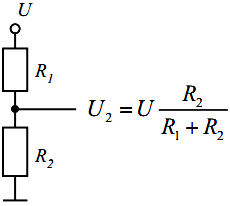
\includegraphics[width=0.25\linewidth]{fig/10-voltage_divider}

\subsubsection{RC és RLC hálózatok}
\paragraph{Soros RC hálózat} esetén az \emph{áramerősség} a közös mennyiség. A feszültségvektorok diagramjából impedancia háromszöget kapunk, melyből Z kiszámíthatjuk a $Z$ impedanciát:
$$Z^2 = R^2 + X_c^2 \rightarrow Z = \sqrt{R^2 + X_c^2}$$
$X_c$-vel a kondenzátor reaktanciája.
A kapcsolás kis frekvencián $X_c$ miatt szakadásként, nagy frekvencián vezetőként, ohmos ellenállásként viselkedik. Határfrekvenciának ($f_h$) nevezzük az áramkörben folyó váltakozó áram azon frekvenciáját, melynél $ R = X_c$.
\begin{figure}[h]
	\centering
	\begin{subfigure}[b]{0.45\textwidth}
		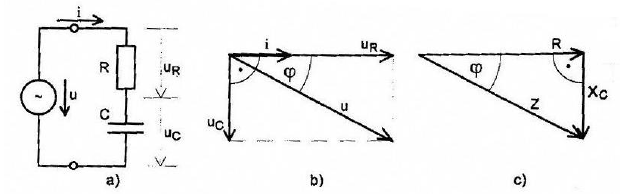
\includegraphics[width=\linewidth]{fig/10-serialRC_Schematic}
		\caption{Soros R-C kapcsolás és vektor diagramja}
		\label{fig:10-serialrcschematic}
	\end{subfigure}
	\begin{subfigure}[b]{0.45\textwidth}
		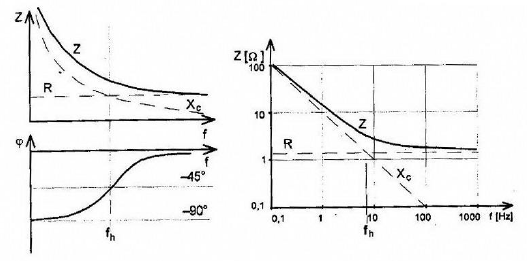
\includegraphics[width=\linewidth]{fig/10-serialRC_Plot}
		\caption{Soros R-C áramkör impedanciájának és fázisszögének változása}
		\label{fig:10-serialrcplot}
	\end{subfigure}
\end{figure}

\paragraph{Párhuzamos RC} hálózatnál a \emph{feszültség} a közös mennyiség. Az áramok vektorainak diagramjából admittancia (Y) háromszöget kapunk:
$$Y^2 = G^2 + B_c^2 \rightarrow Z = \sqrt{G^2 + B_c^2}$$
ahol $B_c = \nicefrac{I_c}{U}$ és $G=\nicefrac{I_R}{U}$.
A kapcsolás kis frekvencián $X_c$ miatt ohmos ellenállásként, nagy frekvencián rövidzárként ($0\Omega$ os ellenállásként) viselkedik. A határfrekvenciát ugyan úgy határozhatjuk meg, mint a soros RC hálózatok esetében.
\begin{figure}[h]
	\centering
	\begin{subfigure}[b]{0.45\textwidth}
		\centering
		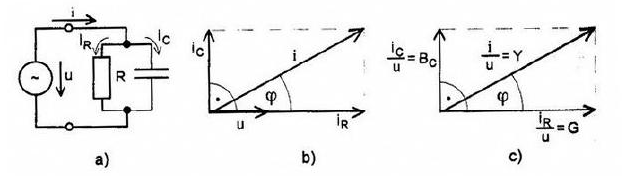
\includegraphics[width=\linewidth]{fig/10-parallelRC_Schematic}
		\caption{Párhuzamos R-C kapcsolás és vektor diagramja}
		\label{fig:10-parallelrcschematic}
	\end{subfigure}
	\begin{subfigure}[b]{0.45\textwidth}
		\centering
		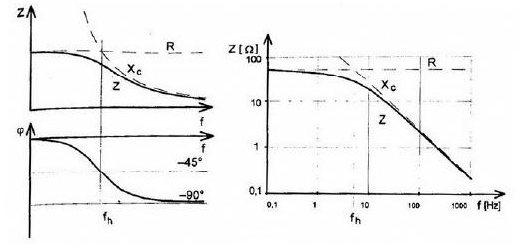
\includegraphics[width=\linewidth]{fig/10-parallelRC_Plot}
		\caption{Párhuzamos R-C áramkör impedanciájának és fázisszögének változása}
		\label{fig:10-parallelrcplot}
	\end{subfigure}
\end{figure}

\paragraph{Soros RLC} Másnéven \emph{sávzáró szűrő}. A soros kapcsolás miatt mindegyik elemen ugyanaz az I áram folyik át, tehát az \emph{áramerősség a közös mennyiség}. Az impedancia háromszög alalpján:
$$ Z = \sqrt{R^2 + (X_L - X_C)^2}$$
ahol $X_L$ és $X_C$ a tekrecs, ill. a kondenzátor reaktanciája.
\begin{figure}[h]
	\centering
	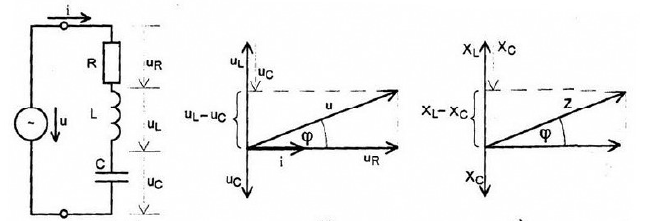
\includegraphics[width=0.5\linewidth]{fig/10-serialRLC}
	\caption{Soros R-L-C kapcsolás és vektor diagramja}
	\label{fig:10-serialrlc}
\end{figure}

\paragraph{Párhuzamos RLC} Másnéven \emph{sáváteresztő szűrő}. Itt a \emph{feszültség} a közös mennyiség. Minden áramot ($I_R, I_L, I_C$) a közös feszültséggel osztva admittancia háromszöget kapunk, melynek alapján:
$$ Y = \sqrt{G^2 + (B_L - B_C)^2}$$
\begin{figure}[h]
	\centering
	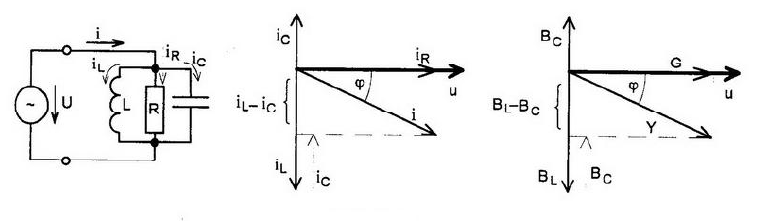
\includegraphics[width=0.5\linewidth]{fig/10-parallelRLC}
	\caption{Párhuzamos R-L-C kapcsolás és vektor diagramja}
	\label{fig:10-parallelrlc}
\end{figure}


\subsection{Diszkrét félvezető eszközök, aktív áramköri elemek, alapkapcsolások.}
\subsubsection{Dióda}
\emph{Egy P és Egy N réteget tartalmaz}. Jelölése kapcsolási rajzon: 
\includegraphics[width=0.2\linewidth]{fig/10-diode}

Működését egyszerűen jellemezhetjük: az egyik irányban engedi folyni az áramot, a másik irányban nem. A jelölés szerint a háromszög irányában folyhat az áram, visszafelé nem. Felhasználásának legáltalánosabb módja az \emph{egyenirányítás}.

A dióda legfőbb jellemzői:
\begin{itemize}[nosep]
	\item rajta átfolyó maximális áramerősség
	\item rajta eső feszültség 
	\item felhasználási terület
\end{itemize}
A diódák általában henger alakúak, két kivezetésük a henger két véglapján található, a rajta levő jelzés alapján megállapíthatjuk melyik vezeték a katód. A diódán az áram az anód irányából a katód irányába folyik (nyitó irányú kapcsolás). Záró irányú kapcsolás esetén elenyészően kicsi áram folyik keresztül a diódán.

A dióda működőképességét ellenállásmérő műszerrel ellenőrizhetjük a következőképpen: mindkét irányban megmérjük az ellenállását. Ha azt tapasztaljuk, hogy az egyik irányban mutat valamekkora ellenállást, a másikban pedig közel végtelen ellenállású akkor a dióda működőképes. A félvezetőkben a szabad töltéshordozók száma és anyag vezetőképessége a hőmérséklettel arányosan változik. Félvezető tulajdonsággal rendelkeznek az alábbi anyagok nagy tisztaságban: germánium (Ge), szilícium (Si), szelén (Se), valamint néhány vegyület: galliumarzenid (GaAs), indiumfoszfid (InP) stb. Nyitóirányú és záróirányú feszültség.(???)%TODO

\paragraph{Zener-dióda}

\includegraphics[width=0.2\linewidth]{fig/10-zener-diode}\\
Stabilizál. Adott nagyságú záróirányú feszültségnél hirtelen megnő a félvezető dióda árama. Konstrukciótól függően különböző letörési feszültségek vannak
\paragraph{Schottky dióda} nagyon gyorsan nyitó/záró dióda típus. Tápegységekben gyakran találkozunk velük.

\subsubsection{Tranzisztorok}
Három kivezetésű félvezető Elektromos jelek erősítésére vagy kapcsolására használják legtöbbet. Egy minimális szintig a tranzisztorok is zárnak, de egy szint fölött telítésbe mennek. E két állapot közötti váltást nevezzük kapcsoló üzemnek, a két szint közötti szakaszon pedig lineáris üzemnek (ilyenkor erősítőként működtetjük). Két elterjedt típusa a bipoláris és a térvezérelt (FET).
\paragraph{Bipoláris tranzisztor}
Nagyjából két dióda egybefordítva. Lehet npn és pnp típusú. Kivezetéseinek neve: kollektor, bázis, emitter. A tranzisztor a bázison átfolyó árammal vezéreljük. Lineáris üzemben a bázisáram változtatásával (ami a bázis és emitter közé kapcsolt nyitófeszültség kis mértékű változtatását jelenti) elérik, hogy a kollektoráram annak ß-szorosával változzon: így hasznosítható a tranzisztor áramerősítése. A lineáris üzemű kapcsolások tervezésnél alapvető lépés a munkapont beállítása. 
Ha a munkapont nincs megfelelő helyen, vagy a jel túl nagy az aktuális munkaponthoz, akkor az erősített kimeneti jel torzított lesz. A tranzisztor könnyen melegszik, és a munkapont eltolódik a hőváltozás hatására, ezért bonyolultabb kapcsolás kell a stabil erősítés eléréséhez.

\paragraph{Térvezérlésű (FET) tranzisztorok}
A kapufeszültség által keltett elektromos tér vezérli, emiatt gyorsabban kapcsolható. Kisebb a hőmérsékletfüggése, és minimális teljesítmény kell a vezérléséhez. Magas a bemeneti impedancia, ezért kisebb zajjal dolgozik, de nem is érhető el vele nagyon nagy erősítés.

\subsubsection{Alapkapcsolások}
A bipoláris tranzisztort négypólusként kezelhetjük, ha három kivezetése közül egyet közösítünk. A bemenet és a kimenet közös pontja földpont. Így váltakozó áramú szempontból három alapkapcsolást különböztetünk meg: közös (vagy földelt) emitteres, közös kollektoros, közös bázisú.
\begin{figure}[h]
	\centering
	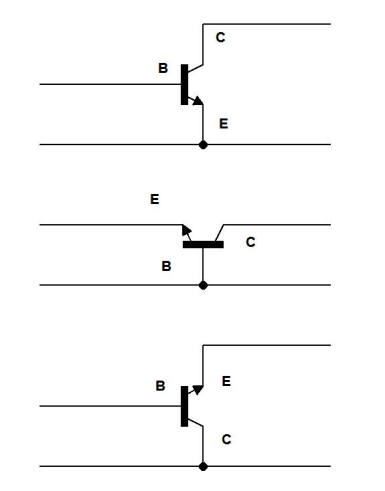
\includegraphics[width=0.5\linewidth]{fig/10-alapkapcs}
	\caption{Tranzisztor alapkapcsolásai}
	\label{fig:10-alapkapcs}
\end{figure}

A tranzisztor működéséhez nyitóirányú bázis-emitter feszültséget (szilícium esetén kb. 0,6 V) kell biztosítani. A kollektor-bázis átmenet előfeszítése záró irányú legyen. Az egyenfeszültségek és egyenáramok a tranzisztor működési állapotának, a munkapontnak az adatai. A munkapont körüli változások jelentik a váltakozó áramú működést. Működés közben egyenáramú és rá szuperponálódott váltakozó áramú mennyiségek mérhetők. 


\subsection{Integrált műveleti erősítők.}
A műveleti erősítő kiváló minőségű differenciálerősítő integrált áramkör, amely egyenfeszültség erősítésére is alkalmas. Analóg számítás- és szabályzástechnikai alkalmazásokhoz fejlesztették ki, de igen sokoldalúan alkalmazzuk őket.\\
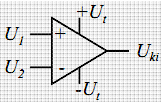
\includegraphics[width=0.25\linewidth]{fig/10-op_amp}\quad
Helyettesítő áramkör: 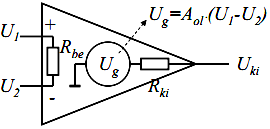
\includegraphics[width=0.5\linewidth]{fig/10-op_amp1}\\

Ideális műveleti erősítő jellemzői:
\begin{itemize}
	\item $U_\text{ki} =A_\text{ol} \cdot (U_1 - U_2)$
	\item Végtelen nagy nyílt hurkú feszültségerősítés ($A_\text{ol} = \infty$)
	\item Végtelen nagy bemeneti ellenállás ($R_\text{be} = \infty$)
	\item Zéró kimeneti ellenállás ($R_\text{ki} = 0$)
	\item Végtelen nagy sávszélesség: minden frekvencián ugyanakkora az erősítése
	\item Zéró ofszet (tökéletesen szimmetrikus felépítés): ha a bemeneti feszültségek megegyeznek, akkor a kimeneti feszültség zéró.
\end{itemize}

Valódi műveleti erősítők jellemző értékei:
\begin{itemize}
	\item szimmetrikus tápfeszültségre van szüksége (tipikusan $\pm 15V$)
	\item $A_\text{ol} \approx 10^5 \text{--} 10^6$
	\item $R_\text{be} \approx 1 \text{--} 200 M\Omega$ bipoláris bemenet, $R_\text{be} \approx 1000 \text{--} 2000 M\Omega$ FET bemenet
	\item $R_\text{ki} \approx 10 \Omega$
	\item $f_\text{min} \approx 0 Hz, f_\text{max} \approx ~\text{MHz}$
	\item közös módusú elnyomási tényező: $\text{CMRR} \approx 90 \text{--} 100 \text{dB}$
	\item véges kimeneti feszültségtartomány: $-U_t < U_\text{ki} < +U_t$
	\item véges maximális jelváltozási sebesség (slew rate): $\text{SR} \approx 0.5 \text{--} 30 \nicefrac{V}{\mu s}$
\end{itemize}

\paragraph{Negatív visszacsatolás} A kimeneti jel egy részét visszavezetik és kivonják a bemeneti jelből, így erősítésre ténylegesen a bejövő jel és az adott hányadban visszacsatolt kimeneti jel különbsége kerül. Így a kimenet megváltoztatása a negatív visszacsatolás révén ellene hat az U’ különbség növekedésének. Állandó bemeneti jel esetén a kimeneti feszültség is stabil értékre áll be. a negatív visszacsatolást alkalmazó áramköröknél a műveleti erősítő két bemeneti feszültségének különbsége a nagy nyílthurkú erősítés miatt igen kicsi.

\begin{figure}[h]
	\centering
	\begin{subfigure}{0.33\linewidth}
		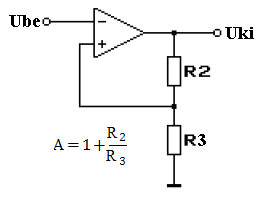
\includegraphics[width=\linewidth]{fig/10-op_amp_neg_invertfeedback}
		\caption{invertáló erősítő}
	\end{subfigure}
	\begin{subfigure}{0.33\linewidth}
		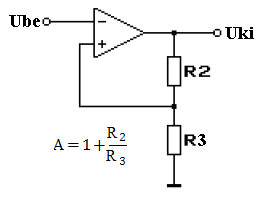
\includegraphics[width=\linewidth]{fig/10-op_amp_neg_noninvertfeedback}
		\caption{nem invertáló erősítő}
	\end{subfigure}
	\begin{subfigure}{0.33\linewidth}
		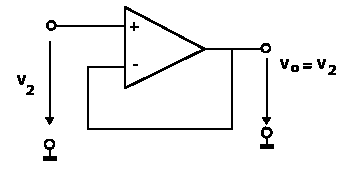
\includegraphics[width=\linewidth]{fig/10-op_amp_neg_voltagefollowerfeedback}
		\caption{feszültségkövető}
	\end{subfigure}
	\caption{műveleti erősítők különböző fajta visszacsatolással}
	\label{fig:10-opampnegfeedbacktypes}
\end{figure}

\subsection{Tápegységek.}
\paragraph{Lineáris üzemű} Transzformátor segítségével átalakítjuk a feszültséget egy számunkra megfelelő szintre, majd egyenirányítjuk. Ezután soros áteresztő elemek (általában tranzisztorok) segítségével szabályozzuk a jelet a stabil kimenet elérése érdekében. Nagy stabilitású kimenetet tudunk vele biztosítani, de a mérete nagy, és a hatásfoka is 20-50\% körül lehet, így nem minden esetben megfelelő.
\paragraph{Kapcsoló üzemű tápegységek} A korábban ismertetett tápegységek (hálózati transzformátor + egyenirányító + áteresztő tranzisztor) hatásfoka csak 25-50\%. Az áteresztő tranzisztor vesztesége jelentősen csökkenthető, ha kapcsolóval helyettesítjük. A transzformátor vesztesége (és mérete) pedig úgy csökkenthető, ha nagyfrekvenciás (20kHz-200kHz) váltakozó feszültséget transzformálnak.

A kapcsoló üzemű tápegységekben (switch-mode power supply (SMPS)) a feszültségszabályozást egy teljesítménytranzisztor változtatható kitöltési tényezővel történő egymást követő bekapcsolásával (teljes telítési állapot) és kikapcsolásával (lezárt állapot) valósítják meg. A terhelésnek megfelelő kitöltési tényezőjű gyorsan ismétlődő (10kHz\textendash100kHz) be- és kikapcsolás a szűrés után a kívánt nagyságú egyenfeszültséget biztosítja a kimeneten

A kapcsolóüzemű (feszültség csökkentő) tápegység működési elve: A K kapcsolót ciklikusan (T periódusidővel) kapcsolgatják: T\textsubscript{be} ideig az 1-es, T\textsubscript{ki} ideig a 2-es potícióba kapcsolják ($T=T be +T_\text{ki}$).

\subsection{Mérőműszerek.}
\begin{description}
	\item[Feszültségmérő] igen nagy belső ellenállású mérőműszer. Párhuzamosan kapcsolandó a mérendő alkatrésszel.
	\item[Áramerősségmérő] igen kis belső ellenállású mérőműszer, az áramkörbe sorosan kapcsolandó.
	\item[Digitális multiméter] Elsősorban egyenfeszültség, egyenáram, ellenállás és kapacitás mérésére használatos. Váltóáram és váltófeszültség effektív értékének mérésére is használható, de csak kisebb frekvenciákon.
	\item[Analóg multiméterek] elektronikus elven működő mérőműszerek,villamos mennyiségek mérésére alkalmasak, a mért mennyiség kijelzése analóg (pl. mutató) műszerrel történik.
	\item[Digitális multiméterek] többfunkciós mérőműszerek, a mért mennyiség számjegyes kijelzővel történik, ehhez mindegyik tartalmaz egy beépített A/D átalakítót és számkijelzőt.
	\item[Oszcilloszkóp] Mind feszültség, mind váltófeszültség mérésére alkalmas. A hagyományos analóg oszcilloszkóp képes megjeleníteni egy periodikus jel időbeli változását és így alkalmas a váltakozófeszültség olyan paramétereinek mérésére, mint pl. a periódusidő, felfutási idő, amplitúdó. Csak periodikus jeleket képesek stabil képpel megjeleníteni. A tárolófunkciós analóg oszcilloszkópok és a digitális oszcilloszkópok egyedi impulzusok megjelenítésére is alkalmasak.
	\item[Analóg oszcilloszkópok] Villamos jelek vizuális vizsgálatát teszi lehetővé egy katódsugárcsöves kijelző segítségével.
	\item[Digitális oszcilloszkópok] Villamos jelek vizuális vizsgálatát teszi lehetővé egy folyadékkristályos kijelző segítségével.
	\item[Szkópméterek] egy kétsugaras digitális tárolóoszcilloszkóp és egy digitális multiméter kombinációja, a mérési funkciók automatikusan a legjobb üzemi állapotra állítódnak be.
\end{description}
%----------------------------------------------------------------------------
\section{Digitális Technika}
{\footnotesize Logikai függvények kapcsolástechnikai megvalósítása. Digitális áramköri családok jellemzői (TTL, CMOS, NMOS). Különböző áramköri családok csatlakoztatása. Kombinációs és szekvenciális hálózatok. A/D és D/A átalakítók.}
%----------------------------------------------------------------------------
\subsection{Logikai függvények kapcsolástechnikai megvalósítása.}
Egy-egy alapáramkör megvalósítására több áramkörtechnikai megoldás született, ezek a teljesítményfelvételben, tápfeszültségigényben, H (high) és L (low) szint feszültségben, sebességben és a kimeneti terhelhetőségben térnek el egymástól. Az áramkörcsaládok helyes megválasztásához ismernünk kell a belső felépítésüket és a bemeneti-kimeneti terhelhetőségüket is. Egy logikai kapu minden bemeneti állapotához meghatározott kimeneti állapot tartozik. A logikai kapu által megvalósított függvény nem egyértelmű, ha a szintállapot és a logikai állapot közötti kapcsolat nincs tisztázva. Ez az összerendelés lehet: pozitív logika (H=1,L=0) és lehet negatív logika (H=0,L=1) ,attól függően, hogy azt az áramkörcsaládot használjuk, amelyikkel egyszerűbb a kapcsolás. Ha negatív logikára térünk át a függvényeket a következőképpen kel megcserélnünk:\\
Nem-vagy $\leftrightarrow$ Nem-és , vagy $\leftrightarrow$ és , nem $\leftrightarrow$ nem\\ 
A fizikai megvalósításukhoz: kapcsolókat,komparátorokat,tranzisztorokat használunk. A gyakorlatban szinte minden logikai kaput Nem-és kapukkal realizálnak, olcsósága miatt.
Egy (kombinációs) logikai áramkör tervezésénél miután felírtuk a függvényt boolean-algebrai alakban, azt egyszerűsítjük. Ezután átírjuk a függvényt úgy, hogy a független változókból képzett maxtermek logikai összege (Diszjunktív normálforma) vagy mintermek logikai szorzata (Konjunktív normálforma) legyen. Ezt az átírást megkönnyíti a Karnaugh--tábla alkalmazása. Az ilyen kanonikus alakra hozott függvény végül a de-morgan azonosságokat felhasználva átírható csak NAND műveleteket tartalmazó formulára.

Négynél több független logikai változó esetén a kézi egyszerűsítés már nem elég hatékony ezért ilyenkor számítógépes algoritmusokat alkalmazunk: Quine-McCluskey (kimerítő teljes algoritmus, melynek hosszú a futásideje, ezért csak közepesen sok változószámig alkalmazható), illetve az Espresso (heurisztikus algoritmus, amit szinte minden szintézisprogram használ) algoritmusok.



\subsection{Digitális áramköri családok jellemzői(TTL, CMOS, NMOS).}
\subsubsection{TTL --- Tranzisztor-tranzisztor logika}
Legnagyobb típus-választékú, univerzális célra készülő bipoláris integrált áramkör rendszer. A bemenetet egy többemitteres tranzisztor szolgáltatja. Kis sebességű, így nagyobb a késleltetés az egyes kapuknál. A fogyasztása a többi családhoz képest elég nagy, de az órajel emelkedésével csak kis mértékben emelkedik és az elektromos kisülések ellen is kellően védett. 

Kis és közepes bonyolultságú integrált áramkörökben a legelterjedtebb bipoláris áramkör. A logikai áramkörökben a kapcsolási és terjedési-késleltetési idők szabják meg a sebességet, a kapunkénti disszipált teljesítmény (fogyasztás) is fontos korlátot szab a rendszernek.
Típusai:
\begin{itemize}[nosep]
	\item H (high speed)
	\item S (schottky-diódás)
	\item L (low power)
	\item LS (low power schottky)
\end{itemize}
\begin{tabular}{|c|c|c|}
	\hline 
	TTL család & Egy kapura eső fogyasztás (mW) & Terjedési-késleltetési idő (ns) \\ 
	\hline 
	normál & 20 & 10 \\ 
	\hline 
	H TTL & 30 & 6 \\ 
	\hline 
	S TTL & 20 & 3 \\ 
	\hline 
	L TTL & 2 & 35 \\ 
	\hline 
	LS TTL & 2 & 15 \\ 
	\hline 
\end{tabular} 
\paragraph{TTL nem-és kapu felépítése és működése:}~\\
U\textsubscript{t} = +5V, L szint: 0V -- 0,8V, H szint: 2,4V -- 5V\\
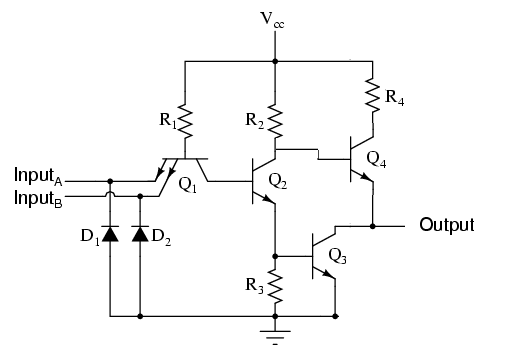
\includegraphics[width=0.5\linewidth]{fig/11-TTL_NAND_schema}
Ha a Q\textsubscript{1} tranzisztor bármelyík emitter kivezetésére 0 logikai szint kerül, a kimeneten 1-es logikai szint lesz a Q\textsubscript{4} tranzisztor és az R\textsubscript{2} ellenállás miatt. Ha a Q\textsubscript{1} tranzisztor mindkét emitter kivezetésére 1 logikai szint kerül, akkor a Q\textsubscript{2} tranzisztor kinyit, a a Q\textsubscript{4} tranzisztor lezár és a Q\textsubscript{3} tranzisztor nyitott állapota miatt alacsony logikai szintre kerül a kimenet.

\subsubsection{MOS --- Metal-Oxid-Semiconductor}
A MOS áramkörök bemenetei érzékenyek a túlfeszültséggel szemben, a megengedettnél nagyobb GATE feszültség miatt átüthet a GATE alatti vékony oxidréteg. Ennél a családnál is tranzisztorokat használnak, de a bipoláris tranzisztorok helyett a fémoxid-félvezetőből készült térvezérlésű FET, vagyis Field-effect tranzisztorokat. Ezáltal sokkal nagyobb műveleti sebességet tudnak elérni.

\subsubsection{N-MOS --- N csatornás MOS (térvezérlésű) tranzisztor}
Csak N-csatornás MOSFET-eket használ, ezáltal csak a magas jelszintet tudja stabilan megjeleníteni. Kisebb a zavarvédettsége és nagyobb a fogyasztása, de a TTL családhoz képest hasonló a CMOS családhoz, csak egyszerűbb kialakítású, ezért olcsóbb is.

Felületigénye jóval kisebb, mint a TTL-nek, gyártási technológiája is gyorsabb (kevesebb művelet), jelentősen kisebb a teljesítményfelvétele. Az N-csatornás tranzisztorok működésében részt vevő Negatív töltéshordozók mozgékonysága majdnem 3-szor nagyobb,mint a (régi technikája miatt kiszorított) P-csatornás tranzisztorok Pozitív töltéshordozóinak mozgékonysága, ezért az N-MOS áramkörök kisebb Gate-kapacitása miatt nagyobb sebességre képesek, csökken a tranzisztor U TO küszöbfeszültsége is, amely alacsonyabb tápfeszültség alkalmazását teszi lehetővé,emiatt könnyebb az N-MOS tranzisztorokat könnyű illeszteni a TTL áramkörökhöz.

\paragraph{N-MOS nem-és kapu felépítése és működése:}~\\

\includegraphics[width=0.5\linewidth]{fig/11-NMOS_NAND_schema1}\\
A T\textsubscript{1} tranzisztort R\textsubscript{D} (100K\textOmega) ellenállás helyett alkalmazzák a térkihasználás és a nagyobb drain ellenállás miatt. Az Y kimeneten csak akkor jelenik meg alacsony logikai színt, ha a T\textsubscript{2} és T\textsubscript{3} tranzisztor is vezet, azaz A-ra és B-re is logikai magas szintet rakunk.

A MOS kapu egyenáramú bemeneti ellenállása nagyon nagy értékű. A bemeneti feszültség változása a gate-kapacitást töltő és kisütő áramot hoz létre. Ez a rövid idejű áramimpulzus nagyobb, mint a szivárgási áram. Ennek ellenére úgy lehet venni, hogy a MOS tranzisztor nem terheli le az előző kapu kimenetét. N-MOS-ok terjedési-késleltetési ideje 15 ns körüli, a teljesítményfelvételük pár szár \textmu W-ig emelkedik.

\subsubsection{C-MOS --- Komplementer MOS tranzisztor}
A működési elve az, hogy N- és P-csatornás MOSFET tranzisztorokat is alkalmaz a logika megvalósításához. A nagy sebesség mellett a fogyasztása is sokkal kisebb a TTL családhoz képest, és a zavarvédettsége is nagyon jó, továbbá széles a működési tápfeszültség tartománya. Egyetlen nagy hátránya, hogy a frekvencia emelkedésével nő a fogyasztása. Működése: egyik helyzetben a felső, P-csatornás tranzisztor nyitott és a kimenetet a pozitív tápfeszültséggel köti össze. A másik helyzetben az alsó, N-csatornás tranzisztor nyit ki és a kimenetet a 0V-tal köti össze. Tehát alacsony jelre a P-MOSFET, magas jelre az N-MOSFET nyit.

A C-MOS-t P-csatornás és N-csatornás növekményes MOS tranzisztorok alkotják.
Jellegzetességei a rendkívülien kis áramfogyasztás, széles működési tápfeszültség-tartomány és a nagy zavarvédettség. A C-MOS áramkörök alapeleme az inverter.

\paragraph{C-MOS nem-és kapu felépítése és működése:}~\\
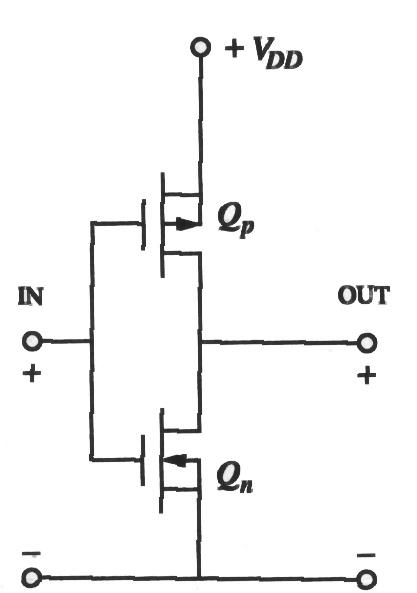
\includegraphics[width=0.5\linewidth]{fig/11-CMOS_NAND_schema}\\
Alacsony logikai bemeneti fesztültségnél az N-csatornás Q\textsubscript{n} tranzisztor lezárt állapotban van és a P-csatornás Q\textsubscript{p} tranzisztor nyitott állapotban így a kimenet logikai magas szinten lesz (megközelítőleg V\textsubscript{DD} értékű). Ha a bemenetre logikai magas szint kerül, akkor Q\textsubscript{n} tranzisztor kinyit és Q\textsubscript{p} tranzisztor lezár, ezáltal logikai alacsony szint kerül a kimenetre. Ha a működési frekvencia megnövekszik, vele együtt nő a teljesítményfelvétel is a tranzisztorok kapcsolási ideje miatt kialakuló tápáramfogyasztás miatt. 

A C-MOS áramkörök tápfeszültsége +3 és +15 V közötti értéket vehet fel. Egy nem-és kapu terjedési késleltetési ideje átlagosan 25 ns, a nyugalmi teljesítmény: 50 nW

A C-MOS áramkörök nagy jelentőségű változata az SOS (Silicon on Sapphire). Szilícium helyett zafír hordozóra alakítják a a C-MOS-okat. Az áramköri elemek között a szigetelési ellenállás nagyon nagy értékű,ezáltal csökken a hordozók kapacitása és nagyságrendekkel nő a sebesség is (1-2 ns). Jelentősen csökken az áramkör nyugalmi teljesítménye is.

\subsection{Különböző áramköri családok csatlakoztatása.}
A logikai függvények fizikai megvalósításához a gyártó cégek bizonyos alapáramkör választékot (családokat) alakítanak ki. Az áramkörök összekapcsolását a katalógusokban található jellemző adataik közlése és egyeztetése teszi lehetővé. A digitális technikában a pozitív logika terjedt el, és az áramkörök pozitív feszültségrendszerben dolgoznak. Amikor
csatlakoztatjuk a különböző áramkörcsaládokat, a következő jellemzőket kell megvizsgálni:
\begin{enumdescript}
	\item[Tápfeszültség] az áramkör működéséhez szükséges feszültség
	\item[Logikai szintek] U\textsubscript{Hmin} és U\textsubscript{Hmax} valamint U\textsubscript{Lmin} és U\textsubscript{Lmax} jellemző értékek
	\item[Zajtartalék, zajérzékenység] feszültségingadozás, ami még nem változtatja meg az állapotot
	\item[Bementeti terhelhetőség] egységterhelés, mind alacsony mind magas logikai szinten
	\item[Kimenteti terhelhetőség] károsodás nélkül a kimenetet képes hajtani
	\item[Teljesítményfelvétel] teljesítményigény 50\%-os terhelésnél
	\item[Jelkésleltetési idő] a kimenet reagál a bemenet hatására, amihez idő kell
\end{enumdescript}

\subsection{Kombinációs és szekvenciális hálózatok. A/D és D/A átalakítók.}
\paragraph{Kombinációs hálózatok} \emph{időfüggetlen} logikai függvényeket valósítanak meg, memória nélküli logikai áramkörök, a kimeneti logikai változókat az adott időpontban megjelenő bemeneti logikai változók határozzák meg, az áramköröket IC-kel (Integrated circuit) valósítják meg, a logikai alapfüggvényeket megvalósító áramköröket logikai kapuknak nevezzük, egy IC-n belül több logikai kapu is található.

\paragraph{Szekvenciális (sorrendi) hálózatok} \emph{időfüggő} logikai függvényeket valósítanak meg, a kimeneti események alakulását a pillanatnyi bemeneti feltételek mellett a korábbi időpillanatokban bekövetkezett kimeneti események is befolyásolják, attól függően, hogy az állapotváltozás hogyan következik be két csoportot különbözetünk meg:
\begin{description}
	\item[Aszinkron] a kimenet előző állapotától való függést visszacsatolással vagy tárolókkal valósítják meg, a kimenet a bemenetre azonnal reagál
	\item[Szinkron] az állapotváltozás a kimeneten egy engedélyező jel (Clock) hatására, azzal azonos fázisban zajlik le, a kimenet előző állapotától való függést tárolókkal oldják meg.
\end{description}

Kombinációs és szekvenciális hálózatok típusai:
\begin{itemize}[nosep]
	\item R-S tároló
	\item Inverz R-S tároló
	\item J-K tároló
	\item T tároló
	\item D tároló
\end{itemize}

\paragraph{A/D átalakítók}
Feladatuk, hogy a bemenetre érkező „A” analóg jelnek megfelelő „D” digitális jelet (bináris számot) állítson elő a kimeneten, a működéshez szükséges egy R referencia (ált. egy U R referenciafeszültség), melyhez a konverter az A analóg mennyiségét viszonyítja és amely a kimeneti feszültség maximális értékét is meghatározza. Az A/D átalakító kvantál (viszonyítási tartományt használ) a digitális jelek előállításához. A digitalizáláshoz elemi lépcsőket kell használni, és minden lépcsőhöz egy digitális mennyiséget (bináris szám) kell rendelni. Az analóg jel annál pontosabban ábrázolható minél kisebb egy elemi lépcső, vagy kvantum nagysága. Az A/D átalakítóknak annál nagyobb a felbontóképessége minél több bit áll rendelkezésre az ábrázoláshoz. Az átalakítók felbontásának növelése az áramköri megvalósítást nehezíti, drágítja. A kis pontosság-igény esetén elég a 8 bit-es (256 elemi lépcső), nagyobb pontosságot biztosítanak a 10,12,14 bites átalakítók és nagy pontosságú rendszerekben 16,18,20 biteseket alkalmaznak.

\paragraph{D/A átalakítók}
Feladatuk, hogy a bemenetre érkező „D” digitális jelnek megfelelő „A” analóg jelet (általában feszültséget vagy áramot) állítson elő a kimeneten, működéséhez szükséges egy U\textsubscript{R} referenciafeszültség (nagyon pontos feszültségforrás), amelyből a kimeneti feszültséget származtatjuk és ez határozza meg a kimeneti feszültség maximális értékét (végkitérését) is. A digitális technikában többnyire bináris alakban állnak rendelkezésre, valamilyen meghatározott kódban kifejezve, ezt a kódot a D/A átalakítónak ismerni kell, csak ezeket a meghatározott bináris kódokat tudják analóg jellé alakítani. Az ideális D/A átalakítók kimeneti jele egyenesen arányos a bemenetükre digitálisan adott szám értékével. A pontosságot itt is az elemi lépcsők száma határozza meg, minél kisebb egy ilyen lépcső, annál pontosabb az átalakítás. Vannak soros és párhuzamos működésű átalakítók és megkülönböztetünk közvetlen és közvetett elvű átalakítókat.

\part[Infokommunikációs hálózatok]{Infokommunikációs hálózatok specializáció}
%----------------------------------------------------------------------------
\section{Távközlő hálózatok}
{\footnotesize Fizikai jelátviteli közegek. Forráskódolás, csatornakódolás és moduláció. Csatornafelosztás és multiplexelési technikák. Vezetékes és a mobil távközlő hálózatok. Műholdas kommunikáció és helymeghatározás.}
%----------------------------------------------------------------------------
\subsection{Fizikai jelátviteli közegek.}

\subsubsection{Koaxiális kábel}
A középponttól a burkolatig haladva az alábbi részekből áll: központi vezeték, dielektrum, árnyékoló réteg, külső műanyag szigetelés.\\
A koncentrikus felépítés miatt kevésbé érzékeny a zavarokra és az áthallásra, mint a csavart érpár. Nagyobb távolságra használható és többpontos alkalmazásban több állomást is képes támogatni (egy közös vonalon).

Egy vezetékre párhuzamosan több kommunikációs eszköz is felszerelhető. 
Analóg átvitel esetén néhány km-enként szükséges erősítés. Mintegy 600 MHz-ig
használható. Digitális átvitel esetén km-enként szükséges jelismétlő használata.
A mai (strukturált kábelezési technológiára épülő) LAN környezetekben már nem
használják új építésű passzív hálózatokhoz.

\subsubsection{Csavart érpár}
A távközlésben alkalmazott kábeltípusok több csavart érpárt tartalmaznak (Számítógép hálózatoknál a 4 érpár szokott lenni). Ezek egy része oda másik része visszirányú információtovábbításra szolgál.

A csavart érpárú kábeleket többféleképpen csoportosíthatjuk. Egyik alapvető különbsége a kábeleknek az árnyékolásuk. Eszerint léteznek árnyékolatlan (UTP), és árnyékolt (FTP,STP) kábeltípusok. Ezen túlmenően a kábelek átviteli jellemzők szerint különböző kategóriákba csoportosítjuk őket:\\
\begin{tabular}{|c|c|c|c|}
	\hline 
	Kategória (USA) & Osztály (EU) & Frekvencia & Bitráta \\ 
	\hline 
	Caetgory 3 & Class C & 16 MHz & 10 Mb/s \\ 
	\hline 
	Cat. 5/5e & Class D & 125 MHz & 100 Mb/s 2 ill. 1 Gb/s 4 érpáron \\ 
	\hline 
	Cat 6 & Class E & 250 MHz & 1 Gb/s 2 érpáron \\ 
	\hline 
	Cat 6a & Class EA & 500 MHz & 10 Gb/s \\ 
	\hline 
	Cat 7 & Class F & 600 MHz & 10 Gb/s \\ 
	\hline 
\end{tabular} 

A csavart érpár kialakításával két dolgot érünk el:
\begin{description}[nosep]
	\item[Zajcsökkentés] A külső zavaró jelek a két, egymáshoz közeli és azonos tulajdonságú dróton megegyező amplitúdóval és fázissal jelennek meg, így a két drót közötti feszültségben a külső jelek hatása nagymértékben kioltja egymást. A csavarásnak köszönhetően a két drót hasonlóan erősen csatolódik a külső jelekhez, hiszen néha az egyik, néha a másik drót van közelebb a zavaró jel forrásához. (Emiatt kell több érpárt más menetemelkedéssel csavarni, hogy ne legyenek minden menetben ugyanúgy összecsatolódva a különböző párok tagjai. Az áthallás így minimalizálható.)
	\item[Vezeték sugárzásának csökkentése] A pár két tagján ellentétes fázisú jelet továbbítva a két drót sugárzása erősen kioltja egymást, így nem fog antennaként viselkedni a kábel.
\end{description}
\subsubsection{Optikai szál}
Egy optikai kábel több szálból tevődik össze, melyek hierarchikusan rendezett nyalábokba vannak szervezve. Épületekben, géptermekben oda-vissza irányú szálpárból (egyenként egycsatornásak) alkotott optikai vezetékeket is használnak. A szálak rétegből tevődnek össze: mag, védőburkolat, puffer, köpeny. 

Egy optikai szál egy vagy több optikai csatorna (WDM) számára használható. Egy csatornás változatban az oda-vissza pont-pont kapcsolathoz két szál szükséges. A fény egy vagy több módusban terjed az optikai szálban eszerint beszélünk egy-módusú (SMF--Singlemode Fibre) és több-módusú (MMF--Multimode Fibre) optikai szálról. Fizikai megnyilvánulásaikban az SMF kábel magja kisebb keresztmetszetű az MMF-éhez képest. Jeltovábbítás tekintetében az SMF jobb, mivel a fény a szál tengelyével párhuzamosan fut visszaverődés nélkül. Emiatt a fényimpulzusok nem torzulnak, nagyobb átviteli sebesség érhető el.

\subsubsection{Rádióhullámok}


\subsection{Forráskódolás, csatornakódolás és moduláció.}


\subsection{Csatornafelosztás és multiplexelési technikák.}


\subsection{Vezetékes és a mobil távközlő hálózatok.}


\subsection{Műholdas kommunikáció és helymeghatározás.}


%----------------------------------------------------------------------------
\section{Hálózatok hatékonyságanalízise}
%----------------------------------------------------------------------------
\subsection{Markov-láncok, születési-kihalási folyamatok.}
A Markov-lánc fogalmához legegyszerűbben a független kísérletek fogalmának általánosításával jutunk el. Tekintsük egymás után végrehajtott  kísérletek sorozatát. Legyen $E_1,E_2,\dots,E_i,\dots$ egy teljes eseményrendszer. Vizsgáljuk az egyes kísérletek eredményét az $E_i$ események bekövetkezése szempontjából. Definiáljuk a $\xi_n\quad(n=0,1,2,\dots)$ valószínűségi változókat úgy, hogy $\xi_n=i$, ha az n-edik kísérletnél az $E_i$ esemény fordul elő.

Független kísérletek esetén érvényes, hogy
$$P(\xi_n=j|\xi_1=i_1,\xi_2=i_2,\dots,\xi_{n-1}=i_{n-i})=P(\xi_n=j)$$
minden n-re, és a szóban forgó valószínűségi változók valamennyi lehetséges értéke. A Markov-lánc fogalmához akkor jutunk, ha a fenti valószínűségeknél feltesszük, hogy a $\xi_n$ változó eloszlása függ az előző $\xi_1,\dots,\xi_{n-1}$ változóktól is.

Ha fennáll minden lehetséges n-re és a változók összes lehetséges értékeire, hogy
$$P(\xi_n=j|\xi_1=i_1,\xi_2=i_2,\dots,\xi_{n-1}=i_{n-i})=P(\xi_n=j|\xi_{n-1}=i_{n-i})$$
úgy azt mondjuk, hogy az egymást követő kísérletek, ill. a $\xi_n$ valószínűségi változók \emph{egyszerű Markov-láncot} alkotnak.

A Markov-láncok fontos speciális esetét képezik a \emph{homogén Markov-láncok}. Ezeknél a  $P(\xi_n=j|\xi_{n-1}=i)$ átmenetvalószínűségek  függetlenek az n-től, azaz
$$P(\xi_n=j|\xi_{n-1}=i)=p_{ij}$$
írható.

Fizikai alkalmazásokat szem előtt tartva a Markov-láncokkal kapcsolatban rendszerint a következő terminológia szokásos: az $E_i$ eseményeket a rendszer \emph{állapotainak} nevezzük. a $\xi_0$ változó $P(\xi_0=i)=P_i(0)$ eloszlást \emph{kezdeti eloszlásnak} és a $P(\xi_n=j|\xi_{n-1}=i)$ feltételes valószínűséget \emph{átmenetvalószínűségnek} nevezzük. Ha pedig $\xi_{n-1}=i$ és $\xi_n=j$ akkor azt mondjuk, hogy a rendszer az n-edik lépésben \emph{átmenetet} tett.

Ha egy Markov-láncnál ismerjük a kezdeti eloszlást és az átmenetvalószínűségeket, úgy ezek segítségével az összes $\xi_n$ változó eloszlása egyértelműen meghatározható.

\subsubsection{Születési-kihalási folyamatok}
A Markov-folyamatok egy igen fontos speciális osztálya születési-halálozási folyamatok néven ismert. A definiáló feltétel: minden állapotból csak "szomszédos" állapotba mehet végbe átmenet ($\pm1$-el változhat). Állapottérnek ekkor a nemnegatív egész számok halmazát választjuk (ami nem megy az általánosság rovására), és $X_k=i$ esetében $X_{k+1}$ vagy $i-1$ vagy $i$ vagy $i+1$ lehet.

Ahhoz, hogy egy $X(t)$ Markov-lánc születési-halálozási folyamat legyen, ki kell elégítenie az alábbi feltételeket:
\begin{enumerate}
	\item $$P(X(t+h)=k+1|X(t)=k)=\lambda_k h+o(h)$$
	\item $$P(X(t+h)=k-1|X(t)=k)=\mu_k h+o(h)$$
	\item $$P(X(t+h)=k|X(t)=k)=1-(\lambda_k+\mu_k)h+o(h)$$
	\item $$P(X(t+h)=m|X(t)=k)=o(h)\quad |m-k|>1$$
\end{enumerate}
ahol $h$ egy tetszőleges kis intervallumot jelent, $o(h)$ pedig olyan mennyiséget jelöl, amely gyorsabban tart 0-hoz, mint $h$, ahogy $h$ nullához tart, vagyis
$$\frac{o(h)}{h}\to 0 ,\quad \text{ha} h\to0$$

Vegyük észre, hogy $\lambda_k,\mu_k$ pozitív mennyiségek függetlenek az időtől. A $\lambda_k$-kat \emph{születési intenzitásnak}, a $\mu_k$-kat pedig \emph{halálozási intenzitásnak} nevezzük.

Jelöljük $P_k(t)$-vel annak a valószínűségét, hogy a folyamat a $t$ időpillanatban a $k$ állapotban van, vagyis
$$P_k(t)=P(X(t)=k)$$
Ezt szokás \emph{abszolút valószínűségnek} is nevezni. Ezen valószínűségek kiszámításához figyelembe kell venni a következőket: A $t+h$ időpillanatban az $X(t)$ $k$ állapotban van akkor és csak akkor, ha az alábbi feltételek teljesülnek:
\begin{enumerate}
	\item $t$ időpillanatban a folyamat a $k$ állapotban van, és a $(t,t+h)$ időintervallumban változás nem következik be
	\item $t$ időpillanatban a folyamat a $k-1$ állapotban volt, és a $k$-ba történt átmenet
	\item $t$ időpillanatban a folyamat a $k+1$ állapotban volt, és a $k$-ba történt átmenet
	\item $(t,t+h)$ alatt 2 vagy több átmenet történt.
\end{enumerate}
Látható, hogy az 1-3 feltételek kölcsönösen kizárják egymást és a 4. eset valószínűsége $o(h)$. Világos, hogy $t$ minden értékére teljes eseményrendszerről van szó, így:
$$\sum_{k=0}^{\infty}P_k(t)=1$$
Az előbbi feltételek teljesülése után mára felírhatjuk a $P_k(t+h)$ valószínűséget:
$$P_k(t+h)=P_k(t)\{1-\lambda_k h-o(h)\}+P_{k-1}(t)\{\lambda_{k-1} h+o(h)\}+P_{k+1}(t)\{\mu_{k+1} h+o(h)\}+o(h),\quad k\ge1$$

\subsection{A legalapvetőbb sorbanállási rendszerek vizsgálata.}
\subsubsection{Rendszerjellemzők}

\paragraph{Kendall-féle jelölés: N/A/B/m/K}~\\
N: igényforrások száma\\
A: beérkezési időközök eloszlása\\
B: kiszolgálási időközök eloszlása\\
m: a kiszolgálók száma\\
K: a várakozási sor kapacitása

\subsubsection{M/M/1}
Az M/M/1 rendszer a legegyszerűbb nemtriviális rendszer. A beérkezési folyamat \textbf{$\lambda$ paraméterű Poisson--folyamat}, vagyis a beérkezési időközök \emph{$\lambda$ paraméterű exponenciális eloszlású} valószínűségi változók.

A kiszolgálási időközök $\mu$ paraméterű exponenciális eloszlású valószínűségi változók. feltesszük továbbá, hogy a beérkezési időközök és a kiszolgálási idők egymástól független valószínűségi változók.

Az ergodikusság szükséges és elégséges feltétele az M/M/1 sor eseten egyszerűen
$$\lambda<\mu,\quad P_0 = 1-\frac{\lambda}{\mu}$$
A kihasználtsági tényező: $\rho=\frac{\lambda}{\mu}$\\
A k.-adik állapot valószínűsége:
$$P_k=(1-\rho)\rho^k \quad k=0,1,2,\dots$$
\paragraph{A rendszer jellemzői}
\begin{description}
	\item[A rendszerben tartózkodó igények átlagos száma] $N=\frac{\rho}{1-\rho}$
	\item[A rendszerben tartózkodó igények átlagos számának szórásnégyzete] $\sigma_N^2=\frac{\rho}{(1-\rho)^2}$
	\item[A várakozó igények átlagos száma (átlagos sorhossz)] $\overline{Q}=\overline{N}-\rho=\frac{\rho^2}{1-\rho}$
	\item[A szerver kihasználtsága] $U_s=1-P_0=\frac{\lambda}{\mu}=\rho$
	\item[A kiszolgáló átlagos foglaltsági periódushossza:] $E_\delta=\frac{1}{\lambda}\cdot\frac{\rho}{1-\rho}=\frac{1}{\lambda}\overline{N}=\frac{1}{\mu-\lambda}$
\end{description}
\subparagraph{Little-formulák}
$$\lambda T=\lambda\frac{1}{\mu(1-\rho)}=\frac{\rho}{1-\rho}=\overline{N}$$
$$\lambda \overline{W}=\lambda\frac{\rho}{\mu(1-\rho)}=\frac{\rho^2}{1-\rho}=\overline{Q}$$

\subsubsection{M/M/1/K}
Rögzített a várakozó igények számának maximuma. Felteszük, hogy a rendszerben legfeljebb K igény tartózkodhat (beleértve a kiszolgálás alatt álló igényt is). Az ezen felül érkező igények nem kerül be a rendszerbe, azonnal távozik, nem kerül kiszolgálásra. Továbbra is \textbf{Poisson--folyamat} szerint érkeznek az igények, azonban csak azok az igények léphetnek be a rendszerbe, amelyek érkezésekor a rendszer állapota kisebb, mint K.

$$\lambda_k=
\begin{cases}
\lambda, & \text{ha } k<K\\
0, & \text{ha } k\geq K 
\end{cases}$$
$$ \mu_k=\mu \quad k=1,2,\dots,K$$
Látszik, hogy ez a rendszer mindig ergodikus, mert állapottere véges. Továbbá:
$$P_k = 
\begin{cases}
P_0\prod_{j=0}^{k-1}\frac{\lambda}{\mu}=P_0(\frac{\lambda}{\mu})^k & \text{ha }k\leq K\\
0 & \text{ha }k>K
\end{cases}$$
$$P_0 = \frac{1-\nicefrac{\lambda}{\mu}}{1-(\nicefrac{\lambda}{\mu})^{K+1}}$$
K=1 esetén a M/M/1/1 rendszer azt jelenti, hogy egyáltalán nincs várakozás.

\subsubsection{M/M/N}
A rendszer n db kiszolgálócsatornával (szerverrel) van ellátva.
Az ergodikusság feltétele: $\frac{\lambda}{n\mu}<1$\\
Ha $k<n$:
$$P_k=P_0(\frac{\lambda}{\mu})^k\frac{1}{k!}$$
Ha viszont $k\geq n$:
$$P_K=P_0(\frac{\lambda}{\mu})^k\frac{1}{n!n^{k-n}}$$

\subsection{A rendszerjellemzők meghatározásának módszerei, meghatározásuk számítógépes támogatása.}

\subsubsection{M/M/n/n -- Elang-féle veszteséges rendszer}
Az $n$ csatornás rendszerbe Poisson--folyamat szerint érkeznek az igények. Ha van üres csatorna (vagy szerver), az igény kiszolgálása exponenciális időtartalmú $\mu$ paraméterrel. Ha minden kiszolgálóegység foglalt, akkor az igény elvész, azaz nincs sorban állás. Ezen probléma a tömegkiszolgálás egyik legrégebbi problémája, mellyel a XX. század elején a telefonközpontok kihasználtságával kapcsolatban foglalkozott A. K. Erlang és C. Palm.
$$\lambda_k=
\begin{cases}
\lambda & \text{ha } k<n\\
0 & \text{ha } k\geq n
\end{cases}$$
$$\mu_k=k\mu\quad k=1,2,\dots,K$$
Azt mondjuk a rendszer k állapotban van, ha k szerver foglalt, azaz ha k igény tartózkodik a rendszerben.

A folyamat stacionárius eloszlása:
$$P_k=
\begin{cases}
P_0(\frac{\lambda}{\mu})^k\frac{1}{k!} & \text{ha } k\leq n\\
0 & \text{ha } k>n
\end{cases}$$
A normalizáló feltétel miatt:
$$P_0=(\sum_{k=0}^{n}(\frac{\lambda}{\mu})^k\frac{1}{k!})^{-1} \implies
P_k=\frac{\frac{\rho^k}{k!}}{\sum_{i=0}^{n}\frac{\rho^i}{i!}}\quad k\leq n$$
A rendszer egyik jellemzője a $P_n=\nicefrac{\frac{\rho^n}{n!}}{\sum_{k=0}^{n}\frac{\rho^k}{k!}}$ valószínűség, melyet először Erlang vezetett be 1917-ben és \emph{Erlang--féle veszteségformula} vagy \emph{Erlang--féle B formula} néven ismert. Általában $B(n,\nicefrac{\lambda}{\mu}$ szimbólummal jelölik. A $P_n$ valószínűség annak a valószínűsége stacionárius esetben, hogy egy újonnan érkező igényt nem fogad a rendszer, azaz az igény elveszik.

Ez a rendszerjellemző meghatározható rekurzív módon, így a köv. formulával számítógép segítségével gyorsan számolható a $B(n,\rho)$:
\begin{align*}
	B(0,\rho)&=1\\
	B(1,\rho)&=\frac{\rho}{1+\rho}\\
	B(n,\rho)&=\frac{\rho B(n-1,\rho}{1+\rho B(n-1,\rho)}
\end{align*}

További számítógépes segítség a rendszerjellemzők meghatározására a szimuláció. A szimulációs folyamat után statisztikai eszközökkel határozzuk meg a rendszerjellemzőket.


%----------------------------------------------------------------------------
\section{Adatbiztonság}
{\footnotesize Fizikai, ügyviteli és algoritmusos adatvédelem, az informatikai biztonság szabályozása. Kriptográfiai alapfogalmak. Klasszikus titkosító módszerek. Digitális aláírás, a DSA protokoll.}
%----------------------------------------------------------------------------
\subsection{Fizikai, ügyviteli és algoritmusos adatvédelem, az informatikai biztonság szabályozása.}
\begin{definition}[Adatvédelem]
	azon fizikai, ügyviteli és algoritmikus eszközök együttes felhasználását értjük, amelyek segítségével a véletlen adatvesztések és szándékos adatrongálódások és információ kiszivárogtatások megelőzhetők, vagy jelentős mértékben megnehezíthetők
\end{definition}
\paragraph{Fizikai adatvédelem} két lényegi dolgot takar: Egyrészt biztosítani kell az optimális, de legalább a még elfogadható \textbf{üzemi körülményeket} (hőmérséklet, páratartalom, por, tartalék alkatrészek stb.), másrészt pedig a szükséges \textbf{vagyonvédelmi intézkedésekről} sem szabad megfeledkezni. Például: Villamos hálózat helyes kialakítása; Szünetmentes tápegységek használata; Megfelelő szerverterem kialakítása(klimatizálás, füstérzékelés, árnyékolás,\dots); Megfelelő adattároló eszközfajták használata; Betörésvédelem.

\paragraph{Ügyviteli adatvédelem} a folyamatok szabályozásának, a szabályzatoknak a kialakítása és védelme. A fizikai adatvédelem önmagában ugyanis nem elegendő. Példa: hiába zárjuk be a szerverszoba ajtaját, ha a portás beengedi azt, aki egy szerszámos táskával érkezvén arról tájékoztatja, hogy ’zsírozni kell a switcheket’ (social hacking/engineering). Tehát szükséges \textbf{pontosan szabályozni}, hogy \textbf{ki}, \text{mikor}, \textbf{mit} és \textbf{hogyan} tehet meg, illetve nem tehet meg. Szükség van \textbf{informatikai biztonsági szabályzatra} is, amely mindezt egységes módon áttekinti. Megfelelő felhasználó menedzselési rendet kell kialakítani, hogy a felhasználók, hozzáférési jogosultságaik, munkájukból adódó szerepköreik kezelése összhangba hozható legyen. Példák: Feladat- és jogkörök szétválasztása; Hozzáférések és tevékenységek regisztrálása; Személyazonosítás; Hatáskörök és felelősségek szétválasztása vagy átlapolása.

\paragraph{Algoritmikus adatvédelem} feladata olyan programok és eljárások alkalmazása, amelyek segítik az előző két terület feladatait és létrehozzák azokat a számítógépes védelmi funkciókat, amik ezen a területen meggátolják az adatokhoz való illetéktelen hozzáférést és módosítást. Példák: Hálózati azonosítás; \textbf{Titkosítás}; Behatolásvédelem; Automatikus adatmentés; Többforrásos adattárolás.

\paragraph{Az informatikai biztonsági szabályrendszer szükségessége:} (1) az adatok egyre inkább elektronikus formában jelennek meg; (2) a Szervezetek informatika nélkül működésképtelenek; (3) az informatikai függőség egyre nagyobb; (4) ugyanakkor a fenyegetettség is egyre növekszik; (5) az üzletfolytonossághoz kritikus fontosságú; (6) a kárpotenciál és a kockázati tényezők szervezetenként eltérőek lehetnek!

\subsubsection{Biztonsági célok}
Alapkövetelmények, amelyek teljesülése az üzemszerű használhatóság előfeltétele:
\begin{enumerate}
	\item rendelkezésre állás (elérhetőség az arra jogosultak számára)
	\item sértetlenség (valódiság)
	\item bizalmasság (jellegtől függően)
	\item nyomon követhetőség, hitelesség
	\item Biztosítékok (az információs rendszer teljességére nézve)
\end{enumerate}
Ez alapján úgy lehet meghatározni az Informatikai Biztonság fogalmát, hogy az akkor áll fenn, ha az információs rendszer védelme az alapkövetelmények szempontjából
\begin{itemize}
	\item \textbf{zárt:} minden fontos fenyegetést figyelembe vesz
	\item \textbf{teljes körű:} a rendszer összes elemére kiterjedő
	\item \textbf{folyamatos:} megszakítás nélküli, az időben változó körülmények ellenére is
	\item \textbf{kockázatarányos:} a feltehető kárérték és a kár valószínűségének szorzata nem haladhat meg egy előre rögzített küszöböt, amely egy üzleti döntés.
\end{itemize}

\subsection{Kriptográfiai alapfogalmak.}



\subsection{Klasszikus titkosító módszerek.}


\subsection{Digitális aláírás, a DSA protokoll.}

%----------------------------------------------------------------------------
\section{A RIP protokoll működése és paramétereinek beállítása (konfigurációja).}

%----------------------------------------------------------------------------

%----------------------------------------------------------------------------
\section{Bevezetés a Cisco eszközök programozásába 1}
{\footnotesize A forgalomszűrés, forgalomszabályozás (Trafficfiltering, ACL) céljai és beállítása (konfigurációja) egy választott példa alapján.}
%----------------------------------------------------------------------------
\subsection{A forgalomszűrés, forgalomszabályozás (Trafficfiltering, ACL) céljai és beállítása (konfigurációja) egy választott példa alapján.}
A rendszergazdáknak meg kell találniuk annak a módját, hogy megakadályozzák a hálózat
jogosulatlan elérését, miközben a belső felhasználók számára lehetővé teszik a szükséges
szolgáltatások használatát. Bár a biztonsági eszközök, mint például a jelszavak, a visszahívó
berendezések és a fizikai biztonsági eszközök sok segítséget nyújtanak, gyakran nem
rendelkeznek az alapvető forgalomszűréshez szükséges rugalmassággal és a rendszergazdák
igényeinek megfelelő vezérlési lehetőségekkel. Előfordulhat például a hálózati rendszergazda
lehetővé kívánja tenni a felhasználók számára az internet elérését, de nem akarja, hogy külső
felhasználók telnettel hozzáférhessenek a LAN-hoz.

A forgalomirányítók alapvető forgalomszűrési lehetőségeket biztosítanak, például hozzáférési
listákat (access control list, ACL) az internetes forgalom letiltásához. Az ACL engedélyező és
tiltó utasítások sorozata, melyek címekre vagy felsőbb rétegbeli protokollokra alkalmazhatók.
Ebben a modulban a normál és kiterjesztett ACL-ek használatáról, mint a hálózati forgalom
vezérlési módszeréről fogunk tanulni, továbbá arról, hogyan használhatók az ACL-ek
valamilyen biztonsági megoldás részeként.

Ezenkívül a fejezetben tippek, elgondolások, javaslatok és általános útmutatások is
szerepelnek az ACL-ek használatával, valamint a létrehozásukhoz szükséges parancsokkal és
beállításokkal kapcsolatban. Végül a fejezet példákat mutat a normál és a kiterjesztett ACL-
ekre és a forgalomirányítók interfészein történő alkalmazásukra.

Az ACL-ek akár egyetlen sorból is állhatnak, ha a cél egy adott állomásról származó
csomagok továbbításának engedélyezése, de tartalmazhatják szabályok és feltételek rendkívül
összetett halmazát is, amelyek pontosan megadják az engedélyezett forgalom jellegét, illetve
befolyásolják a forgalomirányító folyamatok teljesítményét.

\subsubsection{A hozzáférési listák működésének alapelvei}
Az ACL-ek feltétellisták, amelyek a forgalomirányító interfészén keresztülhaladó forgalomra
vonatkozóan lépnek érvénybe. Ezek a listák írják elő a forgalomirányító számára, hogy a
csomagokat fogadja el vagy utasítsa vissza. Az elfogadás és a visszautasítás meghatározott
feltételek alapján is történhet. Az ACL-ek segítségével lehetővé válik a forgalom felügyelete,
valamint a hálózatról kiinduló és az oda befutó elérések biztonságossá tétele.

ACL-ek minden irányított protokollhoz létrehozhatók, többek közt az internetprotokollhoz
(IP) és a hálózatközi csomagcseréhez (IPX) is. Az ACL-ek a forgalomirányítón konfigurálva
adott hálózat vagy alhálózat elérhetőségének vezérlésére használhatók.

Az ACL-ek úgy szűrik a hálózati forgalmat, hogy az irányított csomagok továbbítását vagy
eldobását írják elő a forgalomirányító interfészein. A forgalomirányító minden csomagot
megvizsgál annak meghatározásához, hogy azt az ACL-ben meghatározott feltételek szerint
továbbítani vagy eldobni kell. Az ACL-ek a forrás- és a célcímekre, a protokollokra és a
felsőbb rétegbeli portszámokra nézve adnak meg feltételeket.

Az ACL-eket protokollonként, irányonként és portonként kell létrehozni. Ha szabályozni
szeretnénk egy adott interfész forgalmát, akkor a rajta engedélyezett protokollok
mindegyikéhez külön ACL-t kell készíteni. Egy ACL egy interfészen egyszerre csak egy
irány forgalmát szabályozza. Minden irányhoz külön ACL-t kell létrehozni, egyet a kimenő,
egyet pedig a bejövő forgalomhoz. Végül minden interfészen több protokoll és irány is
definiálható. Ha például egy forgalomirányítónak két interfésze van, és ezeken IP, AppleTalk
és IPX alapú forgalom zajlik, akkor 12 külön ACL-t kell rajta létrehozni: minden
protokollhoz egy-egy ACL, szorozva kettővel a kimenő és a bejövő forgalom miatt, szorozva
kettővel, vagyis a portok számával.

ACL-eket többek között a következő okok miatt szokás létrehozni:
\begin{enumerate}[nosep]
	\item Korlátozható a hálózat forgalma, és növelhető a teljesítménye.
	\item Biztosítják a forgalom szabályozását.
	\item Az útvonalfrissítések továbbítása is korlátozható. Ha a hálózati környezet miatt nincs szükség a frissítésekre, sávszélességet lehet megtakarítani.
	\item Alapszintű hálózati hozzáférés-szabályozást biztosítanak. Az ACL-ek engedélyezhetik például a hálózat egy részének elérését egy állomás számára, és megtilthatják egy másiknak. Lehetséges például, hogy az A állomás hozzáférhet a személyzeti osztály hálózatához, míg a B állomásnak ezt megtiltjuk.
	\item Eldönthetjük, hogy milyen típusú forgalom továbbítódjon és milyen törlődjön a forgalomirányító interfészein. Például engedélyezhetjük az elektronikus levelek továbbítását, de a telnetet tilthatjuk.
	\item A rendszergazdák szabályozhatják, hogy az ügyfelek a hálózat mely részeihez férhetnek hozzá.
	\item Ki lehet választani bizonyos állomásokat, és számukra engedélyezni vagy megtiltani a hálózat egy részének elérését.
	\item A felhasználók számára engedélyezni vagy tiltani lehet bizonyos szolgáltatások, például az FTP vagy a HTTP elérését.
\end{enumerate}

Ha egy forgalomirányítón nincsenek ACL-ek megadva, akkor a forgalomirányítóba befutó csomagok mindegyike továbbhaladhat a hálózat bármely része felé.
\begin{figure}[h]
	\centering
	\begin{subfigure}{0.45\linewidth}
		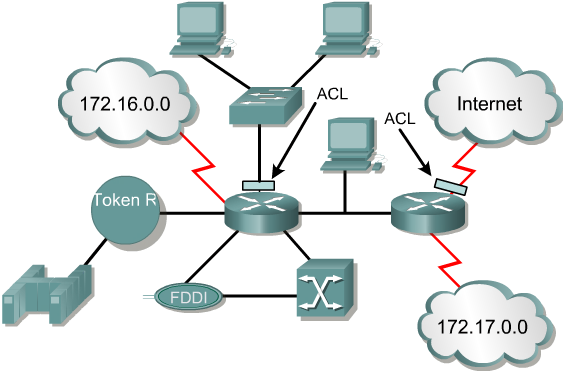
\includegraphics[width=\linewidth]{fig/16-ACL}
		\caption{}
	\end{subfigure}
	\begin{subfigure}{0.45\linewidth}
		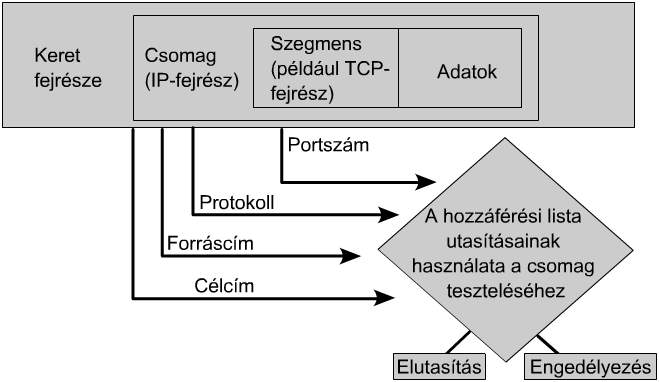
\includegraphics[width=\linewidth]{fig/16-ACL_list-schema}
		\caption{}
	\end{subfigure}
	\caption{}
\end{figure}

\subsubsection{ACL-ek létrehozása}
Az ACL-ek létrehozása globális konfigurációs módban történik.
Számos különböző típusú ACL létezik, így normál, kiterjesztett, IPX, AppleTalk stb. ACL.
Amikor egy forgalomirányítón ACL-eket konfigurálunk, akkor egy-egy szám
hozzárendelésével mindegyiket egyértelműen azonosítanunk kell. A szám megadja az ACL
típusát; ebből következően az adott típushoz tartozó értéktartományba kell esnie:\\
\begin{tabular}{l|l}
	\hline 
	\rule[-1ex]{0pt}{2.5ex} Protokoll & Tartomány \\ 
	\hline 
	\rule[-1ex]{0pt}{2.5ex} IP & 1-99, 1300-1999, 2000-2699 \\ 
	\hline 
	\rule[-1ex]{0pt}{2.5ex} Kiterj. IP & 100-199, 2000-2699 \\ 
	\hline 
	\rule[-1ex]{0pt}{2.5ex} AppleTalk & 600-699 \\ 
	\hline 
	\rule[-1ex]{0pt}{2.5ex} IPX & 800-899 \\ 
	\hline 
	\rule[-1ex]{0pt}{2.5ex} Kiterj. IPX & 900-999 \\ 
	\hline 
	\rule[-1ex]{0pt}{2.5ex} IPX szolgáltatáshirdetés (SAP) & 1000-1099 \\ 
	\hline 
\end{tabular}\\

Miután beléptünk a megfelelő parancsmódba és eldöntöttük, hogy milyen típusú listát
szeretnénk létrehozni, az \verb|access-list| paranccsal, illetve a szükséges paraméterek segítségével
kell megadnunk a hozzáférési lista utasításait.\\
A hozzáférési listák létrehozása az első lépés.\\
A második végrehajtandó művelet a listák hozzárendelése a megfelelő interfészekhez.\\

Az ACL definiálása a következő paranccsal:\\
\verb|Router(config) #access-list access-list-number {permit / deny test-conditions}|

\paragraph{1. lépés:} Az ACL-t egy globális utasítás azonosítja. A normál IP-címekhez az 1-99 tartomány van
fenntartva. Ez a szám mutatja az ACL típusát. A Cisco lOS 11 .2-es verziójától kezdődően az
ACL-ekhez nem csak szám, de név is rendelhető, például oktatasi\_csoport. A globális ACL
utasítás permit illetve deny kifejezése adja meg, hogy a Cisco lOS szoftver hogyan kezelje a
tesztfeltételeket kielégítő csomagokat. A permit általában azt jelenti, hogy a csomag
használhat egy vagy több - később meghatározandó - interfészt. A záró kifejezés(ek) az ACL
állítás által használandó tesztfeltételeket adják meg.

\paragraph{2. lépés:} Ezután alkalmazni kell az ACL-eket egy interfészre az \verb|access-group| paranccsal.\\
Példa: \verb|Router (config-if) #{protocol) access-group access-list number|\\
A hozzáférési lista számával azonosított összes ACL utasítás hozzárendelődik egy vagy több
interfészhez. Az ACL tesztfeltételeket kielégítő csomagok a hozzáférési csoport bármely
interfészét használhatják.

TCP/IP használata esetén az ACL-eket egy vagy több interfészhez lehet hozzárendelni.
Az \verb|ip access-group| parancs segítségével a bejövő vagy a kimenő forgalom szűrésére
állíthatjuk be.

\begin{verbatim}
	Router(config)#access-list 2 deny 172.16.1.1
	Router(config)#access-list 2 permit 172.16.1.0 0.0.0.255
	Router(config)#access-list 2 deny 172.16.0.0 0.0.255.255
	Router(config)#access-list 2 permit 172.0.0.0 0.255.255.255
	Router(config) #interface ethernet 0
	Router(config)#ip access-group 2 in
\end{verbatim}

Az access-group parancsot interfészkonfigurációs módban kell kiadni.
Amikor egy ACL-t hozzárendelünk egy interfészhez, akkor ki kell választanunk, hogy a
bejövő vagy a kimenő forgalomra vonatkozzon. A szűrés tehát az adott interfészre beérkező
és a róla távozó csomagokra vonatkozhat. Annak megállapításához, hogy az ACL a bejövő
vagy a kimenő forgalmat szűrje, az egyes interfészeket a forgalomirányító belsejéből kell
szemlélnünk. Ezt a szemléletet mindvégig meg kell őrizni. A valamilyen interfészen keresztül
beérkező forgalmat bejövő ACL, a kimenő forgalmat pedig kimenő ACL alapján szűrjük.
A számozott ACL-t létrehozása után hozzá kell rendelni egy interfészhez.
Számozott ACL-utasításokat tartalmazó ACL nem módosítható. Előbb törölnünk kell a 
\verb|no access-list lista-szám| paranccsal, majd újra be kell vinnünk a parancsokat.
(\verb|Router(config)#no access-list 2|)\\
Az ACL-ek létrehozásakor és életbe léptetésekor a következő alapvető szabályokat kell
betartani:
\begin{enumerate}[nosep]
	\item Irányonként és protokollonként egy ACL-t kell létrehozni.
	\item A normál hozzáférési listákat a célhoz a lehető legközelebb kell alkalmazni.
	\item A kiterjesztett hozzáférési listákat a forráshoz a lehető legközelebb kell alkalmazni.
	\item A kimenő és a bejövő jelzőket úgy kell használni, mintha a forgalomirányító belsejéből néznénk a portokat.
	\item Az utasítások feldolgozása sorban, a lista tetejétől az alja felé haladva történik, amíg a forgalomirányító egyezést nem talál. Ha nincs egyezés, a forgalomirányító eldobja a csomagot.
	\item Minden hozzáférési lista alján egy implicit deny any (mindent letilt) szabály található. Ez szabály nem jelenik meg az utasításlista alján.
	\item A hozzáférési listák utasításait a specifikusabbaktól az általánosabbak felé haladva kell megadni. Az egyes állomásokra vonatkozó tiltásokat kell először megadni, a csoportokra vonatkozó vagy általános szűrőket utolsóként kell elhelyezni.
	\item Elsőként az egyezési feltétel vizsgálata történik meg. Az engedélyező vagy tiltó részre kizárólag akkor kerül át a vezérlés, ha az egyezés igaz volt.
	\item Soha ne dolgozzunk aktívan működő hozzáférési listával!
	\item Először a logikai utasításokat felvázoló megjegyzéseket készítsük el szövegszerkesztővel, a tényleges végrehajtó műveleteket csak ezt követően írjuk meg.
	\item Az új sorok mindig a hozzáférési lista végére kerülnek. A no access-list x parancs a teljes listát törli. Számozott ACL-ek sorainak egyenként való hozzáadására vagy eltávolítására nincs lehetőség.
	\item Az IP alapú hozzáférési listák a célállomás elérhetetlenségét jelző ICMP-üzenetet küldenek az elutasított csomagok forrásainak, majd a bitszemetesbe dobják a csomagokat.
	\item Hozzáférési lista eltávolítását mindig körültekintően kell végezni. Ha a hozzáférési lista aktív interfészre vonatkozik, és eltávolítjuk, akkor az IOS verziójától függően alapértelmezett tiltó szabály léphet érvénybe az interfészen, ami a forgalom teljes leállását okozza.
	\item A kimenő szűrők nem vonatkoznak a helyi forgalomirányítóról kiinduló forgalomra.
\end{enumerate}

\subsubsection{Normál ACL-ek}
A normál ACL-ek az irányítandó IP-csomagok forráscímét ellenőrzik. Az összehasonlítás a
hálózati, alhálózati és állomáscím alapján egy egész protokollkészlet számára eredményez
engedélyezést vagy tiltást.\\
Például a Fa0/0 interfészen keresztül beérkező csomagok forráscímét és protokollját egyaránt
ellenőrizzük. Ha mindkettő engedélyezve van, a csomagok a forgalomirányítón keresztülvalamelyik kimenő interfészre kerülnek. Ha tiltva vannak, akkor eldobásuk a bejövő
interfészen történik meg.

A globális konfigurációs mód \verb|access-list| parancsának normál változatával normál, 1 és 99
közötti számú ACL definiálható. A Cisco IOS Software Release 12.0.1 és újabb változataiban
a sorszám 1300 és 1999 között is lehet, így akár 798 normál ACL-t is készíthetünk. Ezt az
újabb tartományt kibővített IP ACL-nek nevezzük.

\begin{verbatim}
	access-list 2 deny 172.16.1.1
	access-list 2 permit 172.16.1.0 0.0.0.255
	access—list 2 deny 172.16.0.0 0.0.255.255
	access-list 2 permit 172.0.0.0 0.255.255.255
\end{verbatim}

\begin{itemize}[nosep]
	\item Hozzáférési lista tartományok: I - 99 és 1300 - 1999
	\item Szürés csak az IP-forráscim alapján
	\item Helyettesítö maszkok
	\item A célhoz legközelebbi portra kell alkalmazni
\end{itemize}

Vegyük észre, hogy az első ACL-utasításnál nincs megadva helyettesítő maszk. Ilyenkor a
forgalomirányító az alapértelmezett 0.0.0.0 maszkot használja, vagyis vagy a teljes címnek
egyeznie kell, vagy az ACL ezen sora nem fog illeszkedni, és a forgalomirányító az ACL
következő sorára lép tovább.

A normál ACL-utasítások teljes szintaxisa a következő:\\
{\small\verb+Router(config)#access-list hozzáférési-lista-száma {deny | permit | remark} forrás [forrás-helyettesítő-maszkja] [log]+}

A \verb|remark| (megjegyzés) kulcsszó az ACL-eket könnyebben érthetővé teszi. A megjegyzések
hossza nem haladhatja meg a 100 karaktert.
Példa:
\begin{verbatim}
	access-list 1 remark Csak Jones állomását engedélyezzük
	access-list 1 permit 171.69.2.88
\end{verbatim}

Normál ACL-t törölni a parancs no változatával lehet. Ennek szintaxisa:\\
\verb|Router(config)#no access-list hozzáférési-lista-száma|

Az ip access-group parancs hozzákapcsol egy normál ACL-t egy interfészhez:
\verb+Router(config)#ip access-group {access-list-number | access-list-name} {in | out}+

A táblázat a szintaxisban használt paraméterek leírásait tartalmazza:\\
\begin{tabularx}{\linewidth}{l|X}
	Paraméter & Leírás\\
	\hline
	access-list-nurnber & Az ACL azonosító száma. Decimális szám 1 -99 (normál IP ACL) és 1300 - 1999 (kibővitett IP ACL).\\[1pt]
	deny & Megtagadja a hozzáférést, ha a feltételek teljesülnek.\\[1pt]
	permit & Engedélyezi a hozzáférést, ha a feltételek teljesülnek.\\[1pt]
	remark & A remark (megjegyzés) parancs használata a listák könnyebb megértését és megkeresését segíti.\\[1pt]
	source & Annak a hálózatnak vagy állomásnak a címe, ahonnan a csomagot elküldik. A forrás kétféleképpen adható meg:
		\begin{enumerate}[nosep]
		\item 32 bites cím megadása négy részből álló, pontokkal elválasztott decimális formátumban.
		\item az any kulcsszó a forrás rövidítése: source-wildcard of 0.0.0.0 255.255.255.55.
		\end{enumerate}\\
	source-wildcard & (Opcionális) A forrásra alkalmazandó helyettesítő bitek. A forráshelyettesítő maszkja kétféleképpen adható meg:
	\begin{enumerate}[nosep]
	\item 32 bites cím megadása négy részből álló, pontokkal elválasztott decimális formátumban. A figyelmen kívül agyandó bitpozíciókba 1-et kell írni.
	\item Az any kulcsszó a 0.0.0.0 255.255.255.255 értékű forrás és forráshelyettesítő maszk rövidítése.
	\end{enumerate}\\
	log & (Opcionális) A bejegyzésnek megfelelő csomagról egy tájékoztató célú naplózási üzenet jut a konzolra, (A konzolra küldött naplózási üzenetek részletessége a logging console paranccsal vezérelhető.)Az üzenet tartalmazza az ACL számát, a forráscímet, a csomagok számát és azt, hogy a csomagot engedélyezték-e vagy letiltották. Az üzenet az első megfelelő csomag megtalálásakor generálódik, ezután ötpercenként, megmutatva azoknak a csomagoknak a számát is, amelyek a megelőző öt percben lettek engedélyezve vagy elutasítva.
\end{tabularx}

\subsubsection{Kiterjesztett ACL-ek}
A kiterjesztett ACL-eket a normál ACL-eknél gyakrabban használjuk, mivel szélesebb körű
ellenőrzést tesznek lehetővé.\\
A kiterjesztett ACL-ek a csomagok forrás- és célcímét egyaránt ellenőrzik, illetve a
protokollok és a portszámok egyeztetésére is alkalmasak. Ezek a lehetőségek nagyobb
szabadságot biztosítanak az ACL által vizsgált adatok körülhatárolására. A csomagok
engedélyezése és tiltása forrás, cél, protokolltípus és portszám alapján egyaránt történhet.
Egy kiterjesztett ACL például engedélyezheti az elektronikus levelezést a Fa0/0 interfészről
megadott S0/0 célok felé, miközben tilthatja a fájlátviteleket és a webböngészést. A csomagok
eldobásakor bizonyos protokollok egy visszhangcsomagot küldenek a forrásnak, jelezve, hogy
a cél nem érhető el.

Egy-egy ACL-hez több utasítás is konfigurálható. Az utasítások mindegyikének ugyanazt a
hozzáférési lista számot kell tartalmaznia, így tud hivatkozni az azonos ACL-en belüli
utasításokra. Feltételutasításból tetszőleges számú adható meg, az ilyen utasítások
mennyiségét csak a forgalomirányító memóriájának nagysága korlátozza. Természetesen
minél több az utasítás, annál nehezebb az ACL megértése és kezelése.

A kiterjesztett ACL-utasítások szintaxisa meglehetősen hosszadalmas is lehet, akár a teljes
terminálablakot is kitöltheti. A helyettesítéseknél ugyancsak mód nyílik a host vagy az any
kulcsszó használatára a parancsokon belül.

A kiterjesztett ACL-utasítások végén az opcionálisan megadható TCP vagy UDP
portszámokkal tovább pontosíthatók a szabályok. A TCP/IP protokollkészlet jól ismert
portszámai az ábrán láthatók.\\
{\centering
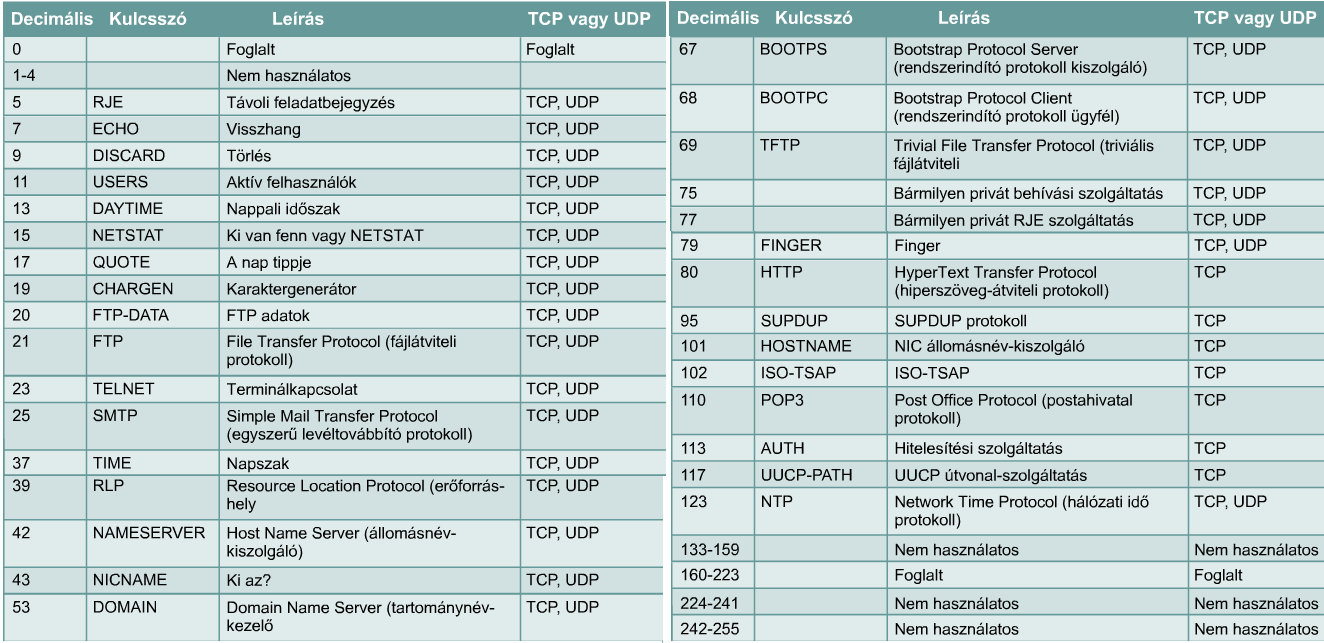
\includegraphics[width=\linewidth]{fig/16-extACL-TCPIP_protocolls}}

A kiterjesztett ACL-ek logikai műveleteket – egyenlő (equal, eq), nem egyenlő (not equal,
neq), nagyobb mint (greater than, gt), kisebb mint (less than, lt) – is képesek végezni a
megadott protokollokon. A kiterjesztett ACL-ek hozzáférési lista száma 100 és 199 között
lehet. (Az újabb IOS-változatoknál a sorszám a 2000–2699 tartományba is tartozhat.)

Az \verb|ip access-group| paranccsal egy meglévő kiterjesztett ACL köthető hozzá egy interfészhez.
Ne feledjük, hogy interfészenként, irányonként és protokollonként csak egy ACL adható meg!
A parancs formátuma: \verb+Router(config-if)#ip access-group hozzáférési-lista-száma {in | out}+

%----------------------------------------------------------------------------
\section{Bevezetés a Cisco eszközök programozásába 2}
{\footnotesize A forgalomirányítási táblázatok felépítése, statikus és dinamikus routing összehasonlítása.}
%----------------------------------------------------------------------------
\subsection{A forgalomirányítási táblázatok felépítése, statikus és dinamikus routing összehasonlítása.}


%\part[Mérés és folyamatirányítás]{Mérés és folyamatirányítás specializáció}
%\input{meres/meres_1}
%\include{meres/meres_2}
%\include{meres/meres_3}
%\include{meres/meres_4}
%\include{meres/meres_5}
%\include{meres/meres_6}

%\part[Vállalati információs rendszerek]{Vállalati információs rendszerek specializáció}
%\input{vir/vir_1}
%\include{vir/vir_2}
%\include{vir/vir_3}
%\include{vir/vir_4}
%\include{vir/vir_5}
%\include{vir/vir_6}

\printindex\addcontentsline{toc}{section}{Tárgymutató}
\end{document}